%% to be called from the project root: file paths are relative to that

\documentclass{book}

\usepackage{xcolor}
\usepackage[
  colorlinks,
  citecolor=green!75!black,
  linkcolor=red!75!black,
  urlcolor=magenta!75!black
]{hyperref}
\usepackage{amsmath}
\usepackage{amssymb}
\usepackage{amsthm}
\usepackage{physics}
\usepackage{breqn}
\usepackage{bbm}
\usepackage[utf8]{inputenc}
\usepackage{graphicx}
\usepackage[margin=1.5in]{geometry}
\usepackage[safeinputenc,authordate,backend=biber]{biblatex-chicago}

%%%%

%% Theorem-like environments

%% http://www.maths.tcd.ie/~dwilkins/LaTeXPrimer/Theorems.html
%% https://www.sharelatex.com/learn/Theorems_and_proofs
%% http://tex.stackexchange.com/a/46262
\newtheorem{theorem}{Theorem}[chapter]
\newtheorem{lemma}[theorem]{Lemma}
\newtheorem{proposition}[theorem]{Proposition}
\newtheorem{corollary}{Corollary}[theorem]
\newtheorem{remark}{Remark}[chapter]
\newcommand{\remarkautorefname}{Remark}

%% Adapted from https://tex.stackexchange.com/q/45817
\theoremstyle{definition}
\newtheorem{definition}{Definition}[section]
\newtheorem{conjecture}{Conjecture}[section]
\newtheorem{example}{Example}[section]

%%%%

%% Misc

\newcommand{\term}[1]{\emph{#1}}
\newcommand{\idop}{\mathbbm{1}}           % Identity operator
\newcommand{\hilb}[1]{\mathcal{#1}}       % Hilbert space
\newcommand{\setof}[1]{\left\{#1\right\}}
\newcommand{\ox}{\otimes}

%% Allows better formatting than \underset
%% https://tex.stackexchange.com/a/130553
\DeclareMathOperator*{\repr}{\equiv}      % represented in a basis, or "has components..."

\renewcommand{\op}{\hat}                  % overwriting physics \op = \ketbra
%\newcommand{\eqbydef}{\coloneqq}
\newcommand{\eqbydef}{\triangleq}
\newcommand{\superop}{\mathcal}

\newcommand{\dket}[1]{\left.\left| #1 \right\rangle\right\rangle}
\newcommand{\Dket}[1]{\left.\left| #1 \right\rangle\!\right\rangle}
\newcommand{\dbra}[1]{\left\langle\left\langle #1 \right|\right.}
\newcommand{\Dbra}[1]{\left\langle\!\left\langle #1 \right|\right.}
\newcommand{\dbraket}[2]{\left\langle\left\langle #1 \middle| #2 \right\rangle\right.\!}
\newcommand{\bradket}[2]{\!\left.\left\langle #1 \middle| #2 \right\rangle\right\rangle}
\newcommand{\braDket}[2]{\!\left.\left\langle #1 \middle| #2 \right\rangle\!\right\rangle}
\newcommand{\dbradket}[2]{\left\langle\left\langle #1 \middle| #2 \right\rangle\right\rangle}
\newcommand{\dketdbra}[2]{\dket{#1}\dbra{#2}}

\newcommand{\pwspace}{\hilb{H}_T \ox \hilb{H}_S}

\NewEnviron{eqsplit}{\begin{equation}\begin{split}\BODY\end{split}\end{equation}}
\NewEnviron{eqsplit*}{\begin{equation*}\begin{split}\BODY\end{split}\end{equation*}}

% Imaginary unit (not used much this way here though)
% https://tex.stackexchange.com/a/303698
\newcommand{\iu}{\mathrm{i}\mkern1mu}
\newcommand{\E}{\mathrm{e}}

\author{Guido De Rosa \\ \small\tt{gderosa@umail.ucc.ie}}
\title{Time as a quantum observable: from Pauli objection to Page and Wootters model --- improvements and applications}

\addbibresource{biblio.bib}


\begin{document}

\frontmatter

\pagenumbering{alph}
\pdfbookmark[chapter]{Front}{front}
\thispagestyle{empty}

NATIONAL UNIVERSITY OF IRELAND, CORK


\includegraphics[width=0.33\linewidth]{img/ucc_logo.pdf}


\pagenumbering{roman}
\maketitle    

\begin{spacing}{1.2}
  \chapter*{Declaration of Authorship}
  \markboth{Declaration of Authorship}{Declaration of Authorship}  %% No ugly "Chapter 0".
  \addcontentsline{toc}{chapter}{Declaration of Authorship}
  This is to certify that the work I am submitting is my own and has not been
submitted for another degree, either at University College Cork or elsewhere. All
external references and sources are clearly acknowledged and identified within the
contents. I have read and understood the regulations of University College Cork
concerning plagiarism.

\hfill

\noindent Student: Guido De Rosa \\
\noindent Date: 22/9/2023

\hfill

\hfill

\noindent \emph{External Examiner}: Prof. J. Gonzalo Muga (Universidad del Pa\'{i}s Vasco)\\
\noindent \emph{Internal Examiner}: Dr. Bryan Kelleher (University College Cork)


  \chapter*{Abstract}
  \markboth{Abstract}{Abstract}  %% No ugly "Chapter 0".
  \addcontentsline{toc}{chapter}{Abstract}
  This work relates to the
\emph{problem of time},
the difficulties of which
represent a classic problem in the foundations of quantum mechanics.
It can be traced back to
the argument, by Wolfgang Pauli,
on the impossibility of defining time as a quantum observable,
due to contradictions related to the specrtum of energy~(1933).
A number of models, aimed at overcoming such difficulties,
have been developed over the decades,
and are reviewed in the present work.

Particular attention is paid to 
the theoretical framework first proposed by Page and Wootters in 1983
(later improved by Lloyd, Giovannetti and Maccone and others),
where time and unitary evolution only emerge in
terms of \emph{entanglement} between non-interacting subsystems
of an otherwise stationary ``universe'',
and where one of the subsystems acts as a ``clock'' for the ``rest'' of it.

\emph{Discrete} clock example, within the framework, are proposed and implemented,
using
existing results related to quantum systems described by finite-dimensional Hilbert spaces.

The formalism is then applied to some simple quantum systems,
and a numerical comparison is performed between the Page--Wootters model and the predictions
of ``ordinary'' quantum mechanics.

The Page and Wootters formalism is also applied to \emph{non-unitary} systems,
such as those modeled in absorption theories of time-of-arrival at a particle detector.
A comparison is made between the predictions of the two models as well.
The case of differing results, among them, potentially opens the way to a future experimental verification.

  \chapter*{}

\vspace{2em}

\begin{flushright}\small
  If only \emph{Bob} could speak, he'd certainly thank \emph{Alice}.
\end{flushright}

  \markboth{}{}

  \chapter*{Acknowledgements}
  \markboth{Acknowledgements}{Acknowledgements}  %% No ugly "Chapter 0".
  \addcontentsline{toc}{chapter}{Acknowledgements}
  {
  I have completed this thesis while still working
  full time as an IT professional and
  software engineer in several companies.
  I want to thank key managers like
  I.~Siddiqui, P. Ryan, M. Taylor, N. Raza, P. Kelleher, A. Ventre, T. Desmond, S.~Sheppard, S. McSherry;
  and some exceptional colleagues and friends:
  we shared a lot about career, life, interests and passions over the years.

  Thanks to my family and friends back in Italy,
  who I am not seeing ---in person--- for a while during this pandemic.

  Thanks to my fellow postgraduate students
  as well as research staff
  at the ``Shortcuts to Adiabaticity'' group.
  A special mention to David Rea.
  I shall acknowledge my supervisor Andreas Ruschhaupt's infinite patience,
  only to name his least ``technical'' quality;
  and his advice against numerous ``traps'' along the journey. And many other reasons.

  Last but not least ---as there's no Bob without Alice in any thought ex\-per\-i\-ment---
  well, Bob would like to thank Alice,
  for every time she’s up when he’s down, and vice versa.
  Their lives might be far apart,
  but they believe in the entanglement,
  and in each other.

  \emph{Cork, February 2021}
}

  {
    \hypersetup{
      linkcolor = .
    }

    % https://tex.stackexchange.com/a/65547
    \cleardoublepage
    \pdfbookmark[chapter]{\contentsname}{toc}
    \tableofcontents
    
    \cleardoublepage
    \pdfbookmark[chapter]{\listfigurename}{lof}
    \listoffigures

    \cleardoublepage
    \pdfbookmark[chapter]{\listtablename}{lot}
    \listoftables
  }
\end{spacing}

\mainmatter

\chapter{Introduction}\label{ch:intro}
\section{Time and the Quantum: An Invitation}\label{sec:intro}

% \begin{savenotes}
\begin{figure}[]
  \centering
  \includegraphics[height=.5\textheight]{img/Shandon_bells_cork.BW.jpg}
  \caption[
    Classical Time. The \emph{Four Faced Liar}, Shandon Bells, Cork
  ]{
    A celebrated example of classical time measurement (and measurement errors) in Cork~City.
    % The \emph{Four Faced Liar}
    % (Shandon Bells, St. Anne's Church, Cork).
    % These four clocks
    % may famously
    % indicate slightly different times from each other.
    ``Each side of the [Shandon Bells] tower also contains a clock face.
    Installed in 1847 and affectionately known as the
    `four-faced liar', the hands on the east and west run slightly fast, especially in windy weather.
    This is probably because they are so very large
    (only Big Ben in London has larger clock faces).''
    \parencite{CorkStrolls}. Photo source: \cite{ShandonBells}.
  }
  %\vspace{3\baselineskip}
  \label{fig:ShandonBells}
\end{figure}
\end{savenotes}

\noindent
Time is a fundamental concept in physics, together with space (or \term{position} within space),
matter (or \emph{mass}) and energy.

In quantum mechanics, at least in first quantization, defining the \emph{position} as
an observable is unproblematic and somewhat basic.
Indeed, representing the quantum state of a particle
in terms of coefficients with respect to eigenstates of position is extremely common.
Almost always when a \emph{wavefunction} $\psi$
for a state $\ket{\psi}$
is written down, the {position representation}
is assumed, unless otherwise (explicitly) noted:
\begin{equation}\label{eq:positionrepr}
  \ket{\psi} = \int \dd{x'} \psi(x') \ket{x'} \text{,}
\end{equation}
where\footnote{
  Here a one-dimensional system is considered, for simplicity:
  it can be easily verified that more dimensions,
  and degeneracy, may be taken into account without altering the key concepts.
}
$\psi(x') = \braket{x'}{\psi}$.

As per \emph{mass}, a quantum mechanism that explains how particle acquire mass was theorized by
Peter Higgs and others in 1964, and confirmed experimentally in 2012
\parencite{Higgs, EnglertBrout, Kibble+, HiggsATLAS, HiggsCMS}.

\emph{Energy}, as an observable, is associated with arguably the most important operator in quantum dynamics: the Hamiltonian.

\emph{Time} is missing from this picture. As of writing of the present work,
there is no general consensus in the physics community on
the definition of a quantum operator associated to a time observable,
or even only on a particular quantum mechanism that would allow time to ``emerge'',
for example, as an effective quantity.

One may argue that the urge of a consistent quantum description for \emph{all} fundamental
measurable quantities, including time,
is essentially (if not purely)
philosophical,
until experiments show (or at least are proposed to show)
``wavelike'' or other nonclassical features of time,
possibly with analogies to what is already observed along the ``position axis''.
Interestingly, accounts exist of experiments, with atomic beams through temporal double-slits,
showing diffraction patterns in time \parencite{TemporalSlits}.
Moreover, signatures of \term{time-crystalline order}
in solids and trapped ions have been recently observed
\parencite{crystal.exp.ordered, crystal.exp.disordered, crystal.exp.nmr, crystal.exp}.

With all the above in mind, the relation between time and other quantities
(whether they are ``quantum observables'' in the formal sense or not)
is explored in the rest of this section,
with reminders about some basic properties that will be useful for the rest of the
discussion.

\subsection{Time and position}

Rigorously speaking, the position observable has no special role in quantum mechanics.
Eq.~\eqref{eq:positionrepr} can be also expanded to
\begin{equation}\label{eq:qprepr}
  \ket{\psi} = \int \dd{x'} \psi(x') \ket{x'} = \int \dd{p'} \tilde{\psi}(p') \ket{p'} \,\text{,}
\end{equation}
with $p$ and $\ket{p}$ being respectively eigenvalues and eigenvectors of the momentum operator.

By multiplying on the left by $\bra{x}$, Eq.~\eqref{eq:positionrepr} yields
\begin{equation}\label{eq:diracdeltax}
  \psi(x) = \int \dd{x'} \psi(x') \delta(x-x') \,\text{.}
\end{equation}
In general, for an observable with continuous spectrum,
in its own eigenbasis, eigenstates are represented as a Dirac deltas
(for discrete spectra, the integral is replaced by a discrete sum,
and Dirac deltas by Kronecker deltas).

Applying the position operator $\hat{X}$ to the~\eqref{eq:positionrepr},
then taking the inner product on the left by $\bra{x}$,
there has
\begin{multline}
  \qty[\hat{X}\psi](x) \eqbydef \mel{x}{\hat{X}}{\psi} =
    \int \dd{x'} \psi(x') x' \mel{x}{\hat{X}}{x'}
    \\
    =
    \int \dd{x'} \psi(x') \delta(x-x') =
    x\psi(x)
  \,\text{.}
\end{multline}
The position
(and an observable in general) is represented, in its own eigenbasis,
simply as the multiplication of the original wavefunction by the respective variable.

\subsection{Time and evolution}

As a matter of experience, if not anything else,
the state of a physical system, either classical or quantum,
with all its observable quantities,
can be regarded as a function of the instant in \emph{time}
(let us call that independent variable $t$).
The same cannot be stated, in general, for any other pair of measurable quantities:
the $x$ coordinate is not a function of the $y$ coordinate
(or their respective statistical amplitudes, in the quantum realm),
and so on.
This status of time as the universally independent variable
has shaped classical mathematical physics: Galilean transformations
do not change time, which remains as an absolute quantity.
The Hamiltonian formalism itself is based on this assumption,
and the Hamiltonian formalism is at the foundation of quantum mechanics too,
which thus inherits ---one may argue--- all the consequences of
treating time as ``external'' with respect to the other quantities under study.
``[The] Hamiltonian method [\dots] marks out a particular time variable
as the canonical conjugate of the Hamiltonian function'' \parencite{DiracLagrangian}.

Emphasizing time as a parameter, the value of a wavefunction
(in position representation, for example)
can therefore be expressed as $\psi_{t}(x)$ at each position $x$
and at each time $t$.
Still, it can be regarded as a function of two variables
and one may wonder why (after an inessential change of notation),
in the identity
\begin{equation}\label{eq:diracdeltaxt}
  \psi(x; t) = \int \dd{x'}\dd{t'} \delta(x-x')\delta(t-t') \psi(x';\, t') \,\text{,}
\end{equation}
the term $\delta(t-t')$ cannot be interpreted as the eigenfunction of some time operator,
which in turn acts as a simple multiplication by $t$ on this
wavefunction $\psi(x; t)$ ---which would be, therefore, a wavefunction in ``time--position representation''.

The fact that $\delta(t-t')$ would be an \emph{improper} eigenfunction
is not the blocking issue in this case (it is not, for the position eigenfunction),
and the mathematical intricacies related to the continuous spectrum are
elegantly resolved by the spectral theory, mainly by Von Neumann
\parencite{VonNeumann}, which is an integral part of the standard, commonly accepted
formulation of quantum mechanics, almost since the early years of the theory.

The main obstacle is instead the \term{Pauli's objection},
which is only indirectly related to the special status of time
as independent variable of ``evolution'', and
directly related to the properties of the spectrum of the {Hamiltonian},
as will be illustrated in Section~\ref{proof}.

\subsection{Time and energy}\label{sec:T--H}

In the quest for a quantum time observable,
it is tempting to leverage
the dualism between position and momentum,
evoked in Eq.~\eqref{eq:qprepr}.
It is well known that the momentum is the infinitesimal generator of spatial translations:
\begin{equation}\label{eq:genspacetransl}
  \psi(x-\Delta x; \, t) = \E^{-\iu \Delta x \hat{P} / \hbar} \psi(x; t) \,\text{,}
\end{equation}
where the momentum operator is $\hat{p} \repr -\iu\hbar \pdv{x}$, in position representation.

It is also well known that the Schr\"odinger equation is equivalent to
stating that the Hamiltonian is the infinitesimal generator of
\emph{temporal} translation:
\begin{equation}\label{eq:gentimetransl}
  \psi(x; t+\Delta t) = \E^{-\iu \Delta t \hat{H} / \hbar} \psi(x; t) \,\text{.}
\end{equation}

The analogy between the two equations above,
among other considerations,
motivates the requirement that
an hypothetical \emph{self-adjoint} time operator should be the canonically conjugate of the Hamiltonian,
just like the momentum operator is canonically conjugate to the position one.
This would involve
a commutation relation between time and energy that is analogous to
the one between position and momentum, $[\hat{X}, \hat{P}] = \iu \hbar$,
and consequently a time--energy uncertainty relation.

Several formulations of such time--energy uncertainty relations have been proposed,
although most of them do not rigorously refer to
a time operator $\hat{T}$ in their definition of $\Delta T$.

On another note, it is worth stressing that,
while equations \eqref{eq:genspacetransl} and \eqref{eq:gentimetransl}
do offer some conceptual motivation towards defining a time observable that is conjugate to the Hamiltonian,
they are not sufficient to logically imply its existence.
Both $\Delta{x}$ and $\Delta{t}$ ---which quantify the spatial and temporal translations at the core of this discussion---
are, once again, mere \emph{parameters} for the \emph{displacement} and \emph{time evolution} operators respectively:
\begin{align}
  \mel{x}{\mathcal{D}_{\Delta{x}}}{\psi(t)}        = \braket{x-\Delta{x}}{\psi(t)}\!\text{, }
    &\text{ with } \mathcal{D}_{\Delta{x}}    = \E^{-\iu \Delta x \hat{P} / \hbar} \\
  \mel{x}{\mathcal{U}_{\Delta{t}}}{\psi(t)}        = \braket{x}{\psi(t+\Delta{t})}\!\text{, }
    &\text{ with } \mathcal{U}_{\Delta{t}}    = \E^{-\iu \Delta t \hat{H} / \hbar}
  \, \text{.}
\end{align}
Even in terms of \emph{position},
$\Delta x$ is not to be intended as the the spread of the $\hat{X}$ operator in this case.
Hence, the analogy between the roles of \emph{parameters} $\Delta x$ and $\Delta t$,
with respect to \emph{operators} $\hat{P}$ and $\hat{H}$,
cannot be used, alone, to rigorously prove the same analogy between the position operator $\hat{X}$
and some time operator $\hat{T}$, although it is somewhat suggestive.

Whether a quantum time observable can be in principle defined as a self-adjoint
operator, or other mathematical frameworks exist that are suitable,
possibly satisfying the above conjugation properties,
is indeed one of the fundamental questions within the entire topic
of the quantization of time.

\subsubsection{Uncertainty relations}

The Heisenberg uncertainty principle is at the core of quantum mechanics.
It was first introduced in 1927 \parencite{Heisenberg:Uncertainty},
in the form of a position--momentum relation: $p_{1}q_{1} \sim h$, in his notation.
Interestingly, in the same paper, Heisenberg also introduced
a \emph{time--energy} uncertainty relation, $E_{1}t_{1} \sim h$,
related to the time at which a transition between two energy levels occurs.

What did Heisenberg mean by $t_1$? Was that an early formalization of (the ``spread'' of)
a time observable (or ``matrix'', in the language of Heisenberg's first formulation of quantum mechanics)?
In fact, the same question can be raised for the position--momentum
relation too. The original formulation of the uncertainty principle
was not expressed in terms of standard deviations and mean values of Hermitian operators
as we know it today. Heisenberg approach was semi-empirical and,
while it turned unsatisfactory from a formal perspective, in some aspects,
it had the merit of explicitly dealing with the physics of the disturbance
of a measurement device to the measurement itself. Therefore,
regardless of the mathematical maturity of its model,
the paper did provide convincing phenomenological arguments towards
the existence of an uncertainty principle for both the position--momentum
\emph{and} the time--energy pair.

As observed in \cite[\s 1.1.3]{TQM1}, Heisenberg introduced the equation
$\mathbf{Et}-\mathbf{tE} = -\iu\hbar$
as ``familiar'', without really specifying the nature of the matrix $\mathbf{t}$,
thus leaving the problem of defining a quantum time observable actually unresolved.
Therein, it is argued that the idea of ``familiarity'' may have originated from the
relation between
the time span and the frequency\footnote{
  Of course, energy and frequency will be often used interchangeably,
  being
  simply related by the the Planck relation $E = h\nu = \hbar\omega$;
  formulated as early as 1900, and incorporated in all the following research
  that brought to the foundation of quantum mechanics, including Heisenberg's work.
}
width of a signal. Regardless of the status
of signal theory in 1927, it is well known, at least in more recent times, that
methods like the Fourier analysis are used in Information and Communication engineering to associate a function in the time domain
to another in the frequency domain; while, in quantum mechanics, the same mathematical operation
is generally used to associate a wavefunction in position representation to
the corresponding one in momentum representation.
This is another suggestive analogy.\footnote{
  In Chapter \ref{ch:pw}, a discrete Fourier transformation will be used indeed to
  associate a time operator to a frequency operator,
  in a modified model of quantum mechanics.
}

Later in 1927, the uncertainty principle was derived in terms of
statistical interpretation of quantum observables
by Kennard and others (see e.g. \cite{Kennard1927}).
The clarification of all formal issues has continued until recently \parencite{Appleby}.
However, all this formalization process has regarded position and momentum only
---not time and energy.

\subsubsection{Mandelstam and Tamm}

The formulation of the time--energy uncertainty relations by Mandelstam and Tamm
\parencite{MandelstamTamm} is considered the least controversial, to the point
of being regularly mentioned in standard textbooks. However,
they refer to the characteristic times of each specific observable $A$ i.e.
the time at which its mean value changes significantly (where ``significantly''
here means: in the order of its spread $\Delta{A}$). So this notion of time
is \emph{observable-dependent} and does not refer to the time (or the statistical spread of time)
at which a particular event happens
---as opposed to the Heisenberg paper, which aimed at answering the question: when does
a ``quantum jump'' occur?

In formulas, the characteristic time is defined by Mandelstam and Tamm as
\begin{equation}
  \tau_{A} = \frac{ \Delta{A} } { \dv*{\langle\hat{A}\rangle}{t} } \, \text{,}
\end{equation}
and the uncertainty relation reads:
\begin{equation}
  \tau_{A}\Delta{E} \ge \frac{\hbar}{2} \, \text{.}
\end{equation}

Some limitations of the Mandelstam--Tamm
approach
will be tackled
in
Chapter \ref{ch:detect}
by further developing
models where time--energy relations have to be intended in the sense
of ``time of occurrence'' (of particle detection)
and time is represented
by a self-adjoint operator.

% [final only] ?? place somewhere else ??? do not use at all ?
% \begin{savenotes}
\begin{figure}[]
  \centering
  \includegraphics[height=.5\textheight]{img/Shandon_bells_cork.BW.jpg}
  \caption[
    Classical Time. The \emph{Four Faced Liar}, Shandon Bells, Cork
  ]{
    A celebrated example of classical time measurement (and measurement errors) in Cork~City.
    % The \emph{Four Faced Liar}
    % (Shandon Bells, St. Anne's Church, Cork).
    % These four clocks
    % may famously
    % indicate slightly different times from each other.
    ``Each side of the [Shandon Bells] tower also contains a clock face.
    Installed in 1847 and affectionately known as the
    `four-faced liar', the hands on the east and west run slightly fast, especially in windy weather.
    This is probably because they are so very large
    (only Big Ben in London has larger clock faces).''
    \parencite{CorkStrolls}. Photo source: \cite{ShandonBells}.
  }
  %\vspace{3\baselineskip}
  \label{fig:ShandonBells}
\end{figure}
\end{savenotes}

\subsection{Time evolution, relativity, photons}\label{sec:trel}

The idea of a perfect analogy between
position--momentum and time--energy uncertainty relations
might naturally lead one to ask whether position and time
(or space and time coordinates), as well as momentum and energy, can be treated on
equal footing. This is what (classically) happens within Einstein's theory of relativity.
Thus, one may further wonder:
would a theory combining quantum mechanics and
relativity be the suitable framework which would allow a rigorous and logically consistent
definition of a time observable,
possibly exposing some analogy with the position operator?

None of the proposed models comprehending both quantum theory and \emph{general} relativity
have reached general consensus,
or the remote possibility of experimental verification \parencite{QGravIntro};
but \term{quantum field theory} (QFT) is an established framework that does combine
some principles
of quantum mechanics with the \emph{special} theory of relativity.

Unfortunately, QFT does not promote time $t$ to some quantum operator $\hat{t}$;
instead, it achieves equal treatment of space and time only by
``demoting'' the \emph{position} operator to a mere classical parameter.\footnote{
  More on this in Section \ref{sec:KG}, where the Klein-Gordon equation is reformulated
  with time as an Hermitian operator in an appropriate Hilbert space
  ---based on the Page--Wootters model, which is introduced in Chapter~\ref{ch:pw}.
}
It treats time and space equally only in the sense that they are all classical,
which appears as the necessary trade-off in order to quantize other quantities
in some mathematically tractable way \parencite[\s I.1]{SrednickiQFT}.

It is no surprise that one of the most successful applications
of QFT, the Standard Model, describes all fundamental interactions except gravity:
while electroweak and strong interactions can be described within a field theory
which treats time and space as a ``background'' (or \emph{labels} to mark the relevant operators),
time and space are expected to be the main mathematical objects (observables),
and transform appropriately,
in a theory of gravity
which has general relativity as its classical counterpart.
Whether the definition of a quantum time operator is an useful step towards
a quantum theory of gravity is, of course, beyond the scope of the present work.

The fact that QFT ``externalizes'' time and position to the rank of classical parameters
is particularly true in quantum electrodynamics, also within the
phenomenology of quantum optics.
Thus it is impossible to define a \emph{photon} position
within standard quantum optics (see, for example, \cite{ScullyZubairy}, sec. 1.5.4 `Wave function for photons'),
and the problem of defining a quantum position observable for a photon
shows an interesting analogy with time for a quantum massive particle.
It is, in fact, a matter of active research \parencite{HawtonPhotonPosition, Hawton2019}.

While there is not a wave function for photons, the wave function for massive particles,
as seen in the Shr\"{o}dinger equation, only exists as a function of position (or momentum, etc.)
but not as a function of time,
i.e. the variable $t$ in Eq.~\eqref{eq:diracdeltaxt}
cannot be regarded as spanning the spectrum of a time operator.

Nevertheless, we have provided an explanation as to why (even without considering the Pauli objection)
relativistic field theories, as currently accepted, cannot provide a solution
to the problem of quantum time, in spite of treating time and space on equal footing,
and despite the fact that position in quantum mechanics is an observable
with its associated self-adjoint operator.

\section{Structure of the thesis}\label{sec:struct}

TODO.

\chapter{Decoherence and Measurement: a review}\label{ch:decohere}
%% With appendices moved here, this chapter is much less
%% about (reletalively recent) research and more
%% textbook-like.

This chapter is devoted to review some
foundations of quantum measurement theory
and is strongly based on works like
\cite{PreskillNotes, Haroche_Exploring, Nakahara, NielsenChuang, open_systems}
where they are presented in the context of
Quantum Information and open systems theory.

\section{Bipartite systems, separable and entangled states}

Consider a \term{bipartite quantum system}
i.e. a composite system $S$
made up of two parts, $A$ and~$B$,
described by their respective Hilbert spaces
$\hilb{H}_A$ and $\hilb{H}_B$.

In \cite{Haroche_Exploring},
a basis for $\hilb{H}_A$ and a basis for $\hilb{H}_B$
are indicated as
$$
  \setof{\ket{i_A}} \text{ and } \setof{\ket{\mu_B}}\,
$$
with Latin and Greek indices to label basis vectors in the two spaces.
This no-\\tation % \footnote{We will partly follow this convention.}
in\-di\-cates potentially different physical roles for the two spaces,
such as the \emph{system of interest} and the surrounding \emph{environment},
or the \emph{system being measured} and the \emph{measurement apparatus}.

If the two subsystems are prepared independently and do not interact with each other,
the system is in a \term{product state} or \term{separable state}:
\begin{equation}\label{eq:separableAB}
  \ket{\psi_S} = \ket{\psi_A}\otimes\ket{\psi_B} \,\text{.}
\end{equation}

It's worth recalling that in a tensor product space $\hilb{H}_A\otimes\hilb{H}_B$
not all vectors can be expressed as a tensor product as in \eqref{eq:separableAB}.
However, the following holds:

\begin{proposition}\label{TensorBase}
The set of tensor products of basis vectors of $\hilb{H}_A$ and $\hilb{H}_B$,
i.e. $$\setof{\ket{i} \otimes \ket{\mu}}_{i\mu},$$
is a basis for $\hilb{H}_A \otimes \hilb{H}_B$.
\end{proposition}
Therefore, we can express any
(generally not separable) state vector of $\hilb{H}_S$
as a \emph{superposition} of separable basis vectors
\begin{equation}\label{eq:bipartite_expansion}
  \ket{\psi_S} = \sum_{i, \mu}\alpha_{i\mu}\ket{i}\otimes\ket{\mu} \text{.}
\end{equation}

\begin{definition}
  Non separable states are defined as \term{entangled}.
\end{definition}

Physically,
$\ket{\psi_S}$ contains information
not only about the results of measurements on $A$ and $B$ separately,
but also on correlations between these measurements.

The simplest example of entangled system is given by two two-level systems,
namely two spin-$\frac{1}{2}$ particles in a singlet state:
\[
  \ket{\psi_{\text{singlet}}} = \frac{1}{\sqrt{2}} \left(\ket{\uparrow, \downarrow} - \ket{\downarrow, \uparrow}\right).
\]

\section{Density operator}\label{app:density}

A quantum state (either pure or \term{mixed}),
is generally described by a \term{density} operator (or density matrix) $\rho$.

The general expression for a density operator $\rho$ is
$$
  \rho = \sum_{k}p_{k}\ketbra{\psi_{k}}
$$
with $p_{k}$ being non negative and $\sum_{k}p_{k} = 1$;
where $p_k$ indicates the ``classical'' probability of the system to be in state $\ket{\psi_{k}}$.

For a pure state (corresponding to ket $\ket{\psi}$) the density operator reduces to
\[
  \rho_{(\text{pure})} = \ketbra{\psi}\,\text{.}
\]

The expectation value of an observable represented by the operator $A$
is given by \parencite{open_systems}
\begin{equation}\label{eq:expvalA_rho}
  \expval{A} = \tr(A\rho)\,.
\end{equation}

Eq. \eqref{eq:expvalA_rho} is valid for any Hermitean operator $A$. Particularly,
it is also valid if $A$ is a \emph{projector} and we will use this
e.g. in Proposition \ref{probability_rho}.

\subsection{Properties of the density operator}
\subsubsection{Additivity}


We can prove the following
\begin{proposition}
  Let $A$ be an hermitean operator such that
  $$
    \tr(A\rho) = 0 
  $$
  \emph{for any density operator} $\rho$.

  It follows that $A = 0$.

  \begin{proof}
    We can choose,
    as basis to explicit the expression of the trace,
    a complete set of eigenvectors $\{\ket{m}\}$ of $A$ and,
    for each positive integer $n$,
    a particular density operator $\rho = \ketbra{n}$,
    corresponding to a (pure) eigenstate of $A$.

    With this particular choice,
    for each $n$,
    $$
      A\rho = \mel{n}{A}{n}\ketbra{n}\,.
    $$
    It then follows:
    \begin{multline*}
      0 = \tr(A\rho) = \sum_{m}\mel{m}{ ( \mel{n}{A}{n}\ketbra{n} ) }{m} = \\
          \sum_{m} \mel{n}{A}{n} \braket{m}{n} \braket{n}{m}
        = \mel{n}{A}{n} ,
    \end{multline*}
    hence the generic diagonal element of the (diagonal) matrix of $A$ is null,
    and so is consequently the operator $A$ itself.
  \end{proof}
\end{proposition}

The \emph{additivity} property follows immediately:

\begin{corollary}
If $\tr(A\rho) + \tr(B\rho) = \tr(C\rho)$ for any density operator $\rho$,
then $A + B = C$.
\end{corollary}

\section{Partial trace and open systems}
\label{sec:p_tr}

In a bipartite system, one subsystem considered alone is an
\emph{open quantum system},
while the system as a whole is still a closed systems.

In this and the following sections, unless differently noted,
we shall stick with the convention of \eqref{eq:bipartite_expansion},
of using
Latin indices for subsystem $A$ and Greek ones for subsystem $B$.

Now, let's consider an observable $M_A$, acting only on subsystems $A$.
It can be expressed in $\hilb{H}_A \otimes \hilb{H}_B$ as
\[
  M_A \otimes \idop_B\, .
\]
Its expectation value is
(using the expansion in eq. \eqref{eq:bipartite_expansion},
and the notation of Latin indices for system $A$ and Greek ones for system $B$)
\begin{multline}\label{eq:exp_subsys}
  \expval{M_A} = \matrixel{\psi_S}{M_A\otimes\idop_B}{\psi_S} = \\[1em]
  \sum_{j,\nu}a^{*}_{j\nu}\left(\bra{j}\otimes\bra{\nu}\right)\left(M_A\otimes\idop_B\right)\sum_{i,\mu}a_{i\mu}\left(\ket{i}\otimes\ket{\mu}\right) = \\
  \sum_{j,\nu,i,\mu}a^{*}_{j\nu}a_{i\mu}\matrixel{j}{M}{i}\matrixel{\mu}{\idop}{\nu} =
  \sum_{j,\mu,i}a^{*}_{j\mu}a_{i\mu}\matrixel{j}{M}{i}
\end{multline}

The bra $\bra{\mu}$, when acting on a ket element of $\hilb{H}_{A} \ox \hilb{H}_{B}$,
can be defined
as a map from $\hilb{H}_A\otimes\hilb{H}_B$ to $\hilb{H}_A$.

A formal definition can be given in terms of how it acts upon a generic
basis ket of $\hilb{H}_A\otimes\hilb{H}_B$.

\begin{definition}\label{def:pBra}
\[
  \braket{\mu}{i\nu} = \bra{\mu}\Big(\ket{i}\otimes\ket{\nu}\Big) \eqbydef \delta_{\mu\nu}\ket{i} \text{.}
\]
\end{definition}

Intuitively, $\bra{\mu}$ is then a ``partial bra''
as it only maps the ``$\ket{\nu}$'' part of\\
``$\ket{i}\otimes\ket{\nu}$''
to a number:
\[
  \begin{array}{cccc}
    \bra{\mu}:  & \ket{i}\ox\ket{\nu}                   & \rightarrow & \delta_{\mu\nu}\ket{i}                \\
                & \rotatebox[origin=c]{270}{$\in$}      &             & \rotatebox[origin=c]{270}{$\in$}      \\
                & \hilb{H}_A\ox\hilb{H}_B               &             & \hilb{H}_A   \text{.}
  \end{array}
\]

This is consistent with the idea of
``tracing out the environment'' within an interpretation where
$\hilb{H}_B$ is the environment, and ultimately with the goal of
studying subsystem $A$ alone in spite of its entanglement with the 
``environment'' (or measurement apparatus etc.) modelled by
subsystem $B$.

Conversely,
the ket $\ket{\mu}$, when acting on a bra element of $\hilb{H}_{A} \ox \hilb{H}_{B}$,
can also be defined
as a map from $\hilb{H}_A\otimes\hilb{H}_B$ to $\hilb{H}_A$.
The following definition of $\ket{\mu}$ is simply \term{dual} to Definition \ref{def:pBra}:
\begin{definition}\label{def:pKet}
  \[
    \braket{i\nu}{\mu} = \Big(\bra{i}\ox\bra{\nu}\Big)\ket{\mu} \eqbydef \delta_{\mu\nu}\bra{i} \text{.}
  \]
\end{definition}
Similar considerations apply:
\[
  \begin{array}{cccc}
    \ket{\mu}:  & \bra{i}\ox\bra{\nu}                   & \rightarrow & \delta_{\mu\nu}\bra{i}               \\
                & \rotatebox[origin=c]{270}{$\in$}      &             & \rotatebox[origin=c]{270}{$\in$}      \\
                & \hilb{H}_A\ox\hilb{H}_B               &             & \hilb{H}_A     \text{.}
  \end{array}
\]

%%

We are now in the position to introduce the \term{partial trace}:
\begin{definition}\label{def:pTr}
  If $\setof{\ket{\mu}}$ is a basis of $\hilb{H}_B$,
  the \term{partial trace}
  is a linear map
  that takes an operator
  $M_{AB}$ on $\hilb{H}_A \otimes \hilb{H}_B$
  to an operator on $\hilb{H}_A$ defined as
  \[
    \tr_B M_{AB} = \sum_{\mu} \matrixel{\mu}{M_{AB}}{\mu}
    \, \text{.}
  \]
\end{definition}

The first thing to note is that the \emph{partial} trace is \emph{operator-valued},
its value is not a scalar as opposed to the \emph{trace}.

Next, we can introduce the \term{reduced density operator}
of system $A$, which is obtained by \emph{tracing out the environment} B,
via the partial trace:
\begin{definition}\label{def:density_A}
  If $\rho$ is the density operator of a whole bipartite system, composed of two parts $A$ and $B$,
  the \term{reduced density operator} related to subsystem $A$ is defined as
  \[
    \rho_A = \tr_B(\rho) \, \text{.}
  \]
\end{definition}

Using the definitions \ref{def:pBra} and \ref{def:pKet}
and the expansion \eqref{eq:bipartite_expansion}, we obtain
\begin{eqsplit}\label{eq:psiPartial}
  \braket{\mu}{\psi_S} &= \sum_i \alpha_{i\mu}    \ket{i} \\
  \braket{\psi_S}{\mu} &= \sum_j \alpha_{j\mu}^{*}\bra{j} \ \text{.}
\end{eqsplit}

which allows us to expand the Definition \ref{def:density_A}
as\footnote{
  Let's recall that the key point of this reasoning is showing how
  a pure state of the total system can correspond to mixed states
  in the two subsystems $A$ and $B$. Therefore, assuming, in what follows,
  that the total state $\rho = \ketbra{\psi}$ is pure, is not restrictive.
}

\begin{equation}\label{eq:density_A_expand}
  \rho_A = \tr_B(\ketbra{\psi_S}{\psi_S}) =
    \sum_{\mu}\braket{\mu}{\psi_S}\braket{\psi_S}{\mu} =
    \sum_{ij\mu} \alpha_{i\mu}\alpha_{j\mu}^{*}\ketbra{i}{j} \text{.}
\end{equation}

Finally, we can see that
\begin{multline*}
  \tr(M_A \rho_A) = \sum_k \mel{k}{M_A \rho_A}{k} =
    \sum_k \mel {k} {M_A \left(\sum_{ij\mu} \alpha_{i\mu}\alpha_{j\mu}^{*}\ketbra{i}{j}\right)} {k} = \\
    \sum_{ijk\mu} \alpha_{i\mu}\alpha_{j\mu}^{*} \mel{k}{M_A}{i} \braket{j}{k} =
    \sum_{ij\mu} \alpha_{i\mu}\alpha_{j\mu}^{*} \mel{j}{M_A}{i}
    \, \text{,}
\end{multline*}
which is the same result as \eqref{eq:exp_subsys}.

This allows us to conclude that
\begin{proposition}
  For an observable $M_A$, acting solely on one subsystem, the expectation value
  for state $\rho$ is given by
  \begin{equation}
    \expval{M_A} = \tr(M_A \rho_A)
  \end{equation}
  where $\rho_A$ is the reduced density operator obtained from $\rho$ by
  tracing out the environment $B$ (as per Definition \ref{def:density_A}).
\end{proposition}

It's clear from \eqref{eq:density_A_expand} that $\rho_A$ is self-adjoint,
hence it can be diagonalized:
\begin{equation}\label{eq:rho_diag}
  \rho_A = \sum_a p_a \ketbra{a}{a} \text{.}
\end{equation}

From \eqref{eq:density_A_expand} we can also derive that
\begin{equation}
  \tr\rho_A = \sum_k \mel{k}{\rho_A}{k} =
    \sum_{ijk\mu}\alpha_{i\mu}\alpha_{j\mu}^{*}\braket{k}{i}\braket{j}{k} =
    \sum_{k\mu}\abs{\alpha_{k\mu}}^2 = 1
\end{equation}
where the last equality is justified by the normalization of $\ket{\psi_S}$
in \eqref{eq:bipartite_expansion}.

The trace, i.e. the sum of matrix diagonal elements, is independent
from the chosen basis, hence $\tr\rho_A = 1$ is valid in particular
for the diagonal form \eqref{eq:rho_diag}, meaning
\[
  \sum_a p_a = 1
\]
and providing a necessary condition to interpret $p_a$ as a probability.

The \eqref{eq:rho_diag}, with $p_a$ as a probability, is often
given as a \emph{definition} of the density operator,
and the \eqref{eq:exp_subsys} can be derived from
such definition alone \parencite{open_systems}.
% TODO: do the calculation?
The probability distribution ${p_a}$
is described as an uncertainty in the preparation of the system
due to an unknown interaction with the environment.

We have seen that a bipartite system, as a whole in a pure state,
can have individual parts in mixed states, due to entanglement between them.

The reverse also holds true:
\begin{proposition}
A system with uncertainties in the preparation of the \emph{state}
(``mixed'') is equivalent to one part (``$A$'') of a bipartite system
entangled with the rest (``B'') such that the total system
$A+B$ is in a pure state.
\end{proposition}

The above is called \term{purification} (see e.g. \cite[sec.2.5]{NielsenChuang}).


\section{(Maximally) mixed state vs (maximally) coherent superposition; diagonal density matrices}

Given, for simplicity, a two-level system (a qubit), and a basis
$\{\ket{0}, \ket{1}\}$, it may be of interest to compare a \term{coherent superposition}
of the two pure states $\ket{0}$ and $\ket{1}$, with equal probability on the outcome of
a measurement (but in a well-defined quantum state); with a statistical mixture of
states $\ket{0}$ and $\ket{1}$, again with equal probability, but 
\emph{in the determination of the quantum state}.

A natural example of such coherent superposition is \parencite[Example 2.4]{Nakahara}
\[
  \ket{\psi} = \frac{1}{\sqrt{2}}\ket{0} + \frac{1}{\sqrt{2}}\ket{1}\text{,}
\]
and the corresponding density operator is
\begin{equation}\label{eq:matrix:pure}
  \rho = \ketbra{\psi}{\psi} =
  \frac{1}{2}\qty\Big(\ket{0} + \ket{1}) \qty\Big(\bra{0} + \bra{1}) =
  \frac{1}{2}\sum_{ij=0}^1\ketbra{i}{j} \repr
  \frac{1}{2}
    \begin{pmatrix}
      1 &1  \\
      1 &1  \\
    \end{pmatrix}
  \text{.}
\end{equation}
For the statistical mixture, the density operator is, by definition,
\begin{equation}\label{eq:matrix:mix}
  \rho = \frac{1}{2}\ketbra{0}{0} + \frac{1}{2}\ketbra{1}{1} \repr
  \frac{1}{2}
    \begin{pmatrix}
      1 &0  \\
      0 &1  \\
    \end{pmatrix}
  \text{.}
\end{equation}

By comparing matrices in \eqref{eq:matrix:pure} and \eqref{eq:matrix:mix}
we may conclude that the off-diagonal terms in the coherent superposition case
indicate \emph{coherence}; however, density operators are self-adjoint operators
(as linear combination of projectors) and can always be expressed in
diagonal form, including density operators of pure states: but it would be
a particular case of diagonal matrix, where all diagonal elements are zero
except one. Indeed, for a pure state:
\[
  \rho = \ketbra{\psi}{\psi}\text{,}
\]
and recalling the assumption that $\ket{\psi}$ is normalized,
we can always build a basis $\qty{\ket{e_j}}$ including $\ket{e_{j_0}} = \ket{\psi}$
among its elements, therefore the diagonal representation is
\[
  \begin{pmatrix}
    0           &       &       &       &       &           \\
                &\ddots &       &       &       &           \\
                &       &1      &       &       &           \\
                &       &       &\ddots &       &           \\
                &       &       &       &\ddots &           \\
                &       &       &       &       &0
  \end{pmatrix}\text{.}
\]

All the above allows us to conclude what follows:
\begin{remark}
  The density matrix of a pure state is either diag(000\dots1\dots000) or non-diagonal.

  So, except the special/trivial case above, a pure state must have off-diagonal terms.
\end{remark}

It's interesting, as well, to look at ensambles (mixtures)
which are not necessarily made up of orthonormal pure states.
In fact, an ensamble of orthonormal states has ``nothing special'',
and different ensambles may lead to the same density operator.
The diagonalized density matrix just shows the ``orthonormal''
ensamble which, again, has no special physical meaning.

For example, let's consider this orthogonal ensamble (diagonal density matrix):
\[
  \rho_1 = \frac{3}{4}\ketbra{0}{0} + \frac{1}{4}\ketbra{1}{1}
\]
and
\[
  \rho_2 = \frac{1}{2}\ketbra{a}{a} + \frac{1}{2}\ketbra{b}{b}\text{.}
\]
It's easy to prove that $\rho_1 = \rho_2$. This is just a particular
case of a theorem.
\begin{theorem}{(Unitary freedom in the ensemble for density matrices).}
  The sets $\setof{\tilde{\ket{\psi_i}}}$ and $\setof{\tilde{\ket{\phi_j}}}$
  generate the same density operator if and only if there exists
  a unitary matrix $\setof{u_{ij}}$ such that
  \[
    \tilde{\ket{\psi_i}} = \sum_j u_{ij}\tilde{\ket{\phi_j}}
  \]
  where $\tilde{\psi_i}$ and $\tilde{\phi_j}$ are not normalized and
  ``embed'' their probabilities $p_i$ and $q_j$ in their respective ensambles,
  i.e.
  \[
    \tilde{\ket{\psi_i}} = p_{i}\ket{\psi_i}
    \text{ and }\,
    \tilde{\ket{\phi_j}} = q_{j}\ket{\phi_j}
  \]
\end{theorem}
See \cite{NielsenChuang}{Theorem 2.6 and introductory example}
for a more detailed description and a proof of the theorem.

\section{Quantum and the Environment: from Quantum to Classical}
\label{sec:q2c}

In Section \ref{sec:mix} we have considered a simple orthonormal basis
and built a statistical mixture of their vectors. We have shown
that the same density operator can be generated by other ensembles,
not necessarily orthogonal. Nonetheless, the orthonormal ensemble,
corresponding to a diagonal representation of $\rho_A$, \emph{is}
special, only in the sense that an orthonormal, complete set of
vectors can be seen as the eigenbasis for some observable,
and such representation is particularly expressive if the
interaction with the environment we are considering
(or the entanglement with the other part of a bi-partite system, in other terms)
is a \emph{measurement}.

An ideal measurement (without knowing the outcome) turns
the (sub-)system $A$ from a coherent superposition into a
maximally mixed state like in the examples
\eqref{eq:matrix:pure} and \eqref{eq:matrix:mix}.
In other words, it transforms a quantum superposition into a classical probability
distribution of possible eigenstates (or possible \term{wavefunction collapses}, in other terms).

Historically,
the effort in overcoming the limitations of quantum measurement models,
treating the measurement apparatus as a quantum,
and not a classical system,
was pioneered by J. von Neumann \parencite{VonNeumann}.

As a self-adjoint operator, $\rho_A$ after the interaction
can always be diagonalized, so we can conclude that any
interaction with the environment is the measurement of some
observable $M_A$, at least in the mathematical sense: $M_A$ may or
may not be of any notable physical significance.

With this in mind, we can mention
a novel approach formulated in the last decades aimed at
\emph{deriving}
the Born rule
instead of requiring it as a postulate
\parencite{Zurek_Einselect}.

A key concept in \cite{Zurek_Einselect} is the
\term{environment-induced superselection} or \term{einselection},
i.e. the idea that particular \term{pointer states} are not
perturbed by the \term{environmental monitoring}.
Because of their stability, they can be regarded as
\term{memory states}.

Coherent superpositions of pointer states are not pointer states
themselves, and such \emph{coherence} is destroyed in the process.
Contrary,
or complementary to previous studies, which focused on the effect of
the environment on the system, Zurek's work
focuses on
accessibility of information spread throughout the environment,
noting that observers monitor systems indirectly, by intercepting
small fractions of their environments:
\begin{quote}
\emph{Relaxation and noise are caused by the environment perturbing
the system}, while \emph{decoherence and einselection
are caused by the system perturbing the environment}.
\end{quote}

\section{Generalized Measurement}
Ch.3 Preskill.
\section{Quantum channels and Kraus operators}

We have seen so far that:
\begin{enumerate}
\item
  Given a bipartite system
  described by the Hilbert space
  $\hilb{H}_A\ox\hilb{H}_B$,
  the susbsystem in $\hilb{H}_A$
  is not necessarily in a pure state itself; it
  may have the properties of a mixed state.
  (Section \ref{sec:p_tr}).
\item
  An orthogonal measurement of the bipartite system can realise a
  (non-orthogonal) POVM on $\hilb{H}_A$ alone (Subsection \ref{subsec:POVM}).
\end{enumerate}

It is therefore of interest to study
the evolution (as a density matrix in $\hilb{H}_A$) of subsystem $A$ alone,
while the bipartite system as a whole evolve unitarily.

The system $A$ alone
(initially described by the density operator $\rho=\ketbra{\psi}$)
can be studied by tracing out $B$
(in the sense of Section \ref{sec:p_tr}),
or equivalently by measuring $B$
but without recording an outcome, therefore leaving the system
in a statistical mixture.
In either ways, there has:
\begin{equation}\label{eq:channel}
  \rho \rightarrow \superop{E}(\rho) \eqbydef \sum_a M_a \rho M_a^{\dagger}
\end{equation}
which generalises the unitary evolution $\rho \rightarrow U \rho U^{\dagger}$.

The linear map, or ``superoperator'',\footnote{
  A \emph{superoperator} is a linear map that associates an operator
  in a Hilbert space to another operator (instead of a vector to another vector).
}
$\superop{E}$
is called \term{quantum channel}.\footnote{
  Another name for it is
  \term{trace-preserving completely positive map},
  or \term{TPCP map} for short. \parencite[sec.3.2]{PreskillNotes}
}
The word ``channel'' is drawn from communication theory,
as the state $\rho$ can be interpreted as being \emph{transmitted}
through
a communication link from a sender to another party
who receives it modified into the state $\superop{E}(\rho)$.

A quantum channel $\superop{E}$
\begin{enumerate}
  \item is linear:
    $\superop{E}(\alpha\rho_1+\beta\rho_2) = \alpha\superop{E}(\rho_1) + \beta\superop{E}(\rho_2)$;
  \item preserves hermiticity:
    $\rho = \rho^{\dagger} \implies \superop{E}(\rho) = \superop{E}(\rho)^{\dagger}$;
  \item preserves positivity:
    $\rho = \rho^{\dagger} \geq 0 \implies \superop{E}(\rho) \geq 0$;
  \item preserves trace:
    $\tr(\superop{E}(\rho)) = \tr(\rho)$.  
\end{enumerate}

Expressing $\superop{E}$ in terms of operators $M_a$
satisfying the partition of the identity \eqref{eq:POVM}
is called
\term{operator-sum representation} of the quantum channel.

The operators $\setof{M_a}$ are called the \term{Kraus operators}
of the channel.

Similarly to POVM $\setof{E_a}$, given a particular channel $\superop{E}$,
the set $\setof{M_a}$ is not uniquely determined, but
generally exists.

A fundamental comparison with unitary evolution is that
quantum channels can be \emph{composed} too, but an inverse
does not generally exists.
This mathematically corresponds to the concept of \term{semigroup},
and physically to the \emph{irreversibility} of the process
of entanglement of subsystem $A$ with the environment. In other words,
there isn't a quantum channel that will bring back an entangled,
mixed state back to its initial pure state;
but a generalized evolution from time $t_0$ to time $t_1$,
described by $\superop{E}_1$,
and another from $t_1$ to $t_2$ described by $\superop{E}_2$
can be combined to describe the evolution from $t_0$ to $t_2$:
\[
  \rho \rightarrow \qty(\superop{E}_1 \circ \superop{E}_2) (\rho) =
  \sum_{\mu,a} N_{\mu} M_a \rho M_a^{\dagger} N_{\mu}^{\dagger}
  \,\text{.}
\]
If we demand that $\superop{E}_1 \circ \superop{E}_2$
is the identity (or ``superidentity'', should we say),
in other words that $\superop{E}_2$
is the \term{inverse} of $\superop{E}_1$,
we can prove that the channel must be unitary i.e.
$\superop{E}_1(\rho) = U \rho U^{\dagger}$
for some unitary evolution operator $U$.
This excludes decoherence,
or entanglement with environment from an initial pure state,
from being reversible.
See \cite[sec.3.2]{PreskillNotes} for a detailed proof,
and general properties of quantum channels.


\chapter{Pauli's objection and historical developments}\label{ch:hist}
\section{Pauli's objection}\label{proof}

The existence of a time operator with the properties required in Section \ref{sec:T--H}
is hindered by a fundamental objection
which was raised by W.~Pauli for the first time
in his \term{General Principles of Quantum Mechanics}, dated 1933,
where he argued that the existence of a self-adjoint operator,
conjugate to the Hamiltonian,
would lead to absurd consequences on the energy spectrum.
He did not provide a formal proof of his argument,
and only relegated his observation into a footnote
of his work
\parencite{PauliFootnote}; but that was sufficient to
lead most physicists to insist that ``time is just a parameter''
in quantum mechanics
since then.

Here we aim at providing
a more technical proof of Pauli's ``theorem'',
based on some relatively recent work by
E. Galapon \parencite{Galapon2002},
while expanding some details further.
A preliminary Lemma on commutator algebra follows.

\begin{lemma}\label{CommProp}
  If the commutator $[T, H]$ commutes with $T$ i.e.
  $$[T, H]T~=~T[T, H]\,,$$ then the following holds:
  \begin{equation}\label{eq:tkh}
  [T^k, H] = kT^{k-1}[T, H]\,.
  \end{equation}
  \end{lemma}
  This is particularly true when $[T, H]$ is a \emph{number} as in \eqref{THcommutator} where
  $T$ and $H$ are the time and energy operator respectively.
  \begin{proof}
  First of all, the \eqref{eq:tkh} is trivially valid for $k = 1$.

  For an arbitrary positive integer $k > 1$ there has:
  \begin{dmath}\label{tkhrecur}
  [T^k, H] = T^{k-1}TH - HT^{k-1}T = T^{k-1}TH - T^{k-1}HT + T^{k-1}HT - HT^{k-1}T \\
      = T^{k-1}[T, H] + [T^{k-1}, H]T
  \end{dmath}
  Now, iterating the result in \eqref{tkhrecur},
  \begin{dmath}\label{tkhrecurplus}
  [T^k, H] = T^{k-1}[T, H] + [T^{k-1}, H]T
  = T^{k-1}[T, H] + (T^{k-2}[T, H] + [T^{k-2}, H]T)T
  = T^{k-1}[T, H] +  T^{k-1}[T, H] + [T^{k-2}, H]T^2
  = 2T^{k-1}[T, H] + [T^{k-2}, H]T^2
  = \hdots
  = nT^{k-1}[T, H] + [T^{k-n}, H]T^n = \hdots
  \end{dmath}
  where the commutativity hypothesis $[T, H]T = T[T, H]$ has been used to obtain
  $$T^{k-2}[T, H]T = T^{k-1}[T, H]\text{.}$$

  Now, \eqref{tkhrecurplus} can be continued until it reaches $n=k$ when the term
  $[T^{k-n}, H]T^n$ vanishes and a result of $kT^{k-1}[T, H]$ follows.
  \end{proof}
\normalsize

Let us now come to the Pauli argument; and
assume that there exists a self-adjoint time operator, $T$, canonically conjugate
to the Hamiltonian $H$, i.e.

\begin{equation}
\label{THcommutator}
[T, H] = i\hbar
\end{equation}
Since T is self-adjoint, then for all
$\beta\in\mathbb{R}$, $U_{\beta} = \exp(- i \beta T / \hbar)$
is unitary. A formal
expansion of the exponential yields the commutator

\begin{equation}\label{eq:pauli_sum}
[U_{\beta}, H]  =
\left[
  \sum_{k=0}^{\infty} \frac{1}{k!} \left(- \frac{i\beta T}{\hbar} \right)^k, H
\right]         =
\sum_{k=0}^{\infty} \frac{1}{k!} \left(- \frac{i\beta}{\hbar} \right)^k [T^k, H] \,\text{.}
\end{equation}

As the commutator $[T, H]$ itself commutes with its operator $T$,
the following identity holds (see Lemma \ref{CommProp}):

$$
[T^k, H] = kT^{k-1}[T, H]
$$
hence:

\begin{multline}\label{eq:pauli_sum_w_lemma}
[U_{\beta}, H]  =
\sum_{k=0}^{\infty} \frac{1}{k!} \left(- \frac{i\beta}{\hbar} \right)^k kT^{k-1}[T, H] \\ =
\beta\sum_{k=1}^{\infty} \frac{1}{(k-1)!} \left(- \frac{i\beta}{\hbar} \right)^{k-1} T^{k-1} =
\beta\sum_{\kappa=0}^{\infty} \frac{1}{\kappa!} \left(- \frac{i\beta T}{\hbar} \right)^{\kappa}  =
\beta U_{\beta}
\end{multline}
where the term for $k=0$ in the first sum clearly vanishes, hence we can start the sum from
$k=1$ then set $\kappa=k-1$ in the last step.

Now, given an eigenvector $\varphi_{E}$ of $H$ so that $H\varphi_{E}=E\varphi_{E}$,
using Eq.~\eqref{eq:pauli_sum_w_lemma}, we get

$$
HU_{\beta}\varphi_{E} = (U_{\beta}H - [U_{\beta}, H])\varphi_{E} =
EU_{\beta}\varphi_{E} - \beta U_{\beta}\varphi_{E} = (E-\beta)U_{\beta}\varphi_{E} \, \text{,}
$$
showing that $U_{\beta}\varphi_{E}$ is another eigenvector of $H$ with eigenvalue
$E-\beta$. But $\beta$ is an arbitrary real number and $H$ a \emph{generic} Hamiltonian,
hence the spectrum of a generic Hamiltonian $H$ should
be the whole real line, which contradicts the discrete and semi-bounded energy spectrum
in fact found in most physical systems.

%%

For several decades, Pauli's argument had prevented most theoretical attempts at
defining a self-adjoint
time operator with the required commutation and uncertainty properties.
However, some research effort has been invested
into weakening some of those requirements, 
thus rendering the Pauli objection no longer applicable.

Notable examples of possible approaches involve:
renouncing the self-adjointness of the operator~$\hat{T}$ (replacing it with a more general symmetric operator);
allowing for the corresponding spectral measurement not to be projective (replacing it with a POVM);
or including the case of an \emph{imaginary} potential in the Hamiltonian,
to model absorption by a detector via loss of normalization (non-unitary evolution).

\section{Aharonov--Bohm}

In their 1961 paper, Aharonov and Bohm \parencite{AharonovBohm}
showed that ``energy can be measured
  reproducibly in an arbitrarily short time'',
thus apparently contradicting the time--energy indeterminacy theorized
by
Mandelstam and Tamm (see also Sec. \ref{sec:T--H}) and by other authors.
As observed by Aharonov and Bohm, in the Mandelstam--Tamm derivation, \emph{time} has a different meaning:
it is essentially the lifetime of a system in a particular state
and not the duration of the energy measurement process.
They also critically reviewed previous works by Landau and Peierls \parencite{LandauPeierls}
and by Fock and Krylov \parencite{FockKrylov}, discussed their level of generality and provided
counterexamples to their formulation of the time--energy uncertainty relation.

In their model, they considered a free particle as a ``clock''
and quantize (by symmetrizing the corresponding operators)
the classical relation
$t = y / v = m y / p$
for a particle that is at position $y = 0$ at time $t = 0$ and travels at velocity $v$ along the $y$ axis.
The corresponding time operator has then expression:
\begin{equation}
  \hat{T}_{AB} = \frac{m}{2} \qty( \hat{Y} \frac{1}{\hat{P}_y} + \frac{1}{\hat{P}_y} \hat{Y} ) \,\text{.}
\end{equation}
In the paper, this operator is claimed to be Hermitian, although with a singularity for $p_{y} = 0$.\footnote{
  This is stressed in a footnote of Aharonov--Bohm's paper.
  The reader might have noticed the irony of fundamental historical papers
  relegating important information at the level of footnotes
  ---and the present work, in many parts, not even trying to ``improve'' such a traditional trend.
}
With some simple algebra, a commutation relation $[\hat{H}_{c}, \hat{T}_{AB}] = \iu\hbar$
can be proved, where $\hat{H}_c = \hat{P}_y^2/2m$ is the Hamiltonian of the free particle that is used as a ``clock''.

This seems to contradict Pauli's argument: however, more recent studies
\parencite{MugaAB98, MugaAB99, MugaAB99Err}
have shown that
$\hat{T}_{AB}$ is not, strictly speaking, self-adjoint but ``only'' maximally symmetric
(a weaker and more general condition).
An analogy has been made therein with the momentum on the half-line,
a restriction of the well known momentum operator to a subdomain
that is defined as
$\qty{\psi \in \mathscr{L}^2(\mathbb{R}): \psi(x) = 0 \; \forall x < 0}$ in position representation.
% Removal suggested due to mathematical intricacies...
% As opposed to the momentum in the half-line, $\hat{T}_{AB}$ does not have a self-adjoint extension though.
It has also been shown that the associated spectral measure is not projector valued, but
positive-operator valued (POVM). Projectors are a particular subclass of \term{positive operators}.
Among other applications, suitable positive operators can be used to extend von Neumann decomposition
in order to describe
open quantum systems and ``unsharp'' measurements.

Another apparent contradiction is the commutator $[\hat{H}_{c}, \hat{T}_{AB}] = \iu\hbar$
(and the consequent uncertainty relation $\sigma_{H_{c}} \sigma_{T_{AB}} \geq \frac{\hbar}{2}$)
with Aharonov--Bohm's conclusion that
energy can be measured, in principle, with arbitrary precision in an arbitrarily short time;
but it should be noted that $\hat{H}_{c}$ is the energy of the clock, not of the system under energy-measurement,
thus the contradiction does not hold.

The Aharonov--Bohm model explicitly includes a clock in the description, i.e.,
a different system to the one under measurement;
and this separate system has one of its observables
on a well known dependency upon time, so the corresponding eigenvalues can be seen
as possible positions of the ``hand'' of the clock.
Aharonov and Bohm infer that $\hat{T}_{AB}$ must commute with all the observables
of the main system (and in particular the Hamiltonian, let's call it $\hat{H}_S$),
given that they are defined in different Hilbert spaces:
therefore, there is no
fundamental reason why the system energy represented by $\hat{H}_S$, and the clock time $\hat{T}_{AB}$,
could not have, in the same measurement,
arbitrarily
narrow statistical distributions around some of their eigenvalues.

This idea of a quantum description of time through modeling a ``clock''
(in other words, the notion of time as ``what is shown on a clock'' with some suitable properties)
has a certain historical relevance because later models, independently developed,
have been based on that idea too.
In particular, we can mention
the Page--Wootters model \parencite{PageWootters}, where a peculiar relation is in place between the clock and the system,
of which we will not explore the details at this stage though,
as those will be discussed extensively (with numerical applications, experiments, and comparisons with other models)
in Chapter \ref{ch:pw}.

\input{tex/hist/allcock}
\section{Kijowski}\label{sec:kijowski}

In 1974, Jerzy Kijowski pursued an axiomatic approach towards a
time-of-arrival quantum distribution. In his paper \parencite{Kijowski}, he sought to compute
the probability distribution for a particle to intersect an hypersurface
$\mathcal{Q}$ immersed in the $(3+1)$-dimensional space-time.
Classically, the trajectory of a particle is a curve in this $3+1$ space
which intersects the hypersurface at a certain point $(\bar{t^{\vphantom{1em}}}, \bar{x^1}, \bar{x^2}, \bar{x^3})$.
An example of a purely
space-like hypersurface is defined by an equation like
$t=\bar{t}$ (which is, more specifically, an hyperplane).
The point coordinates
at which the particle passes through it
essentially tell \emph{where}
the particle is at time $\bar{t}$,
i.e. the values of $\bar{x^1}$, $\bar{x^2}$, $\bar{x^3}$,
given that $\bar{t}$ is known.
For a quantum particle, the exact coordinates $\bar{x^1}$, $\bar{x^2}$, $\bar{x^3}$
are replaced by a complex wavefunction $\psi_{\bar{t}} \in \mathscr{L}^2(\mathbb{R}^3)$
of the variables $x^1$, $x^2$, $x^3$,
where:
$\psi_{\bar{t}}(x^1, x^2, x^3) = \braket{x^1, x^2, x^3}{\psi_{\bar{t}}}$;
$\bra{x^1, x^2, x^3}$ is an eigenbra of the 3-dimensional position operator $\bra{x^1} \ox \bra{x^2} \ox \bra{x^3}$;
and $\ket{\psi_{\bar{t}}}$ is the state ket at time $\bar{t}$ in the ordinary quantum mechanics sense.

The probability that the particle hits this hyperplane at its point of coordinates $x^1, x^2, x^3$
is given by the square modulus $\abs{\psi_{\bar{t}}(x^1, x^2, x^3)}^2$.
More generally, probability distributions are given by bilinear functionals of the wavefunction.

Kijowski then considers an hypersurface that is spanned by one time-like vector and two independent
space-like vectors (as opposed to the purely space-like hypersurface mentioned above).
The time coordinate of the intersection with the \term{world line}
of a particle tells \emph{when} the particle traverses the surface.
(Again, in the quantum sense, such exact value shall be replaced by a probability distribution).
One obvious example would be the hyperplane $x^3 = \bar{x^3}$.
Or, more simply, $x^3 = 0$, which we will consider from now on.

Given all the above considerations, the first requirement is:
\begin{axiom}\label{ax:kijowski:first}
  The probability distribution for the time-of-arrival of a particle at a given surface
  is given by a continuous positive bilinear functional
  \begin{equation*}
    F[\psi_{t}] \eqbydef T_F[\psi_{t}, \psi_{t}] \, \text{.}
  \end{equation*}
\end{axiom}

The reader can classically and intuitively picture an horizontal plane,
a particle below it traveling upwards, and ask the question
``when does the particle pass through?''. The point of intersection,
besides the coordinate $\bar{x^3}$ which is known, and the other two space-like coordinates $\bar{x^1}$ and $\bar{x^2}$,
will have the time coordinate $\bar{t}$ which is the \term{time of arrival} at the hypersurface.

Consistently with the above, Kijowski initially restricted the study to
particles with positive momentum, which in terms of momentum wavefunction
obviously means ${\phi(p^1, p^2, p^3) = 0} \,\, {\forall \, p^3 < 0}$.

The momentum representation $\phi$ is, in fact, used the most in Kijowski's
paper, to make the theory explicit. The rest of this Section will reflect that.

Other requirements for the probability distribution $F[\phi_t]$ are
\begin{axiom}
  $F[\phi_t] \ge 0 \ \forall t$
\end{axiom}
\begin{axiom}
  If $\norm{\phi_t}_{\scriptscriptstyle{\mathscr{L}^2(\mathbb{R}^3)}} = 1 \ \forall t$, then $\int F[\phi_t] \dd t = 1$
\end{axiom}
\begin{axiom}
  $F[\pi(\phi)] = F[\phi]$.
\end{axiom}
In the last one, $\pi$
is the representation of any Galilei transformation
which preserves $\mathcal{Q}$
e.g. a translation which is parallel to the surface
(the first Kijowski paper considered the nonrelativistic case).

From now on, we will consider, for simplicity, the surface $x^3 = 0$.

For reasons of symmetry, in terms of time-of-arrival at $x^3 = 0$,
one intuitively expects a particle
``traveling upwards from the bottom'' to be equivalent
to a particle
``traveling downwards from the top'',
if both position and momentum have their sign flipped.
For a quantum wavefunction in the position representation,
this means
replacing $\psi(\va{x})$ with $\psi(-\va{x})$.
Or $\phi(\va{p})$ with $\phi^{*}(\va{p})$ in momentum representation:
\begin{axiom}
  $F[\phi^{*}_t] = F[\phi_t]$, $\forall t$.
\end{axiom}

The last requirement is that
\begin{axiom}\label{ax:kijowski:last}
    The \term{dispersion}, defined as
    \begin{equation}\label{eq:kijowski:dispersion}
      \int \dd{t} t^2 F[\phi_t] - \qty(\int \dd{t} t F[\phi_t] )^2 \text{,}
    \end{equation}
    is finite.
\end{axiom}

Given the above axioms, Kijowski proved the following
\begin{theorem}
  $\,$

  \begin{enumerate}
    \item
      A specific functional $F_0$ which minimizes the variance
      \eqref{eq:kijowski:dispersion}
      exists;
    \item
      The average value $\int \dd{t} t F[\phi_t] $ is constant over the class of
      functionals defined by the axioms;
    \item
      $F_0$ has the expression
      \begin{multline}\label{eq:kijowski_bilinear_full}
        F_0[\phi_t] = T_{F_0}[\phi_t, \phi_t] = \\
            \frac{1}{m(2\pi\hbar)^4}
            \int\displaylimits_{p_{3}', p_{3}'' \ge 0} \sqrt{p_{3}' p_{3}''} \phi_t^{*}(p_1, p_2, p_{3}') \phi_t(p_1, p_2, p_{3}'')
            \dd p_1 \dd p_2 \dd p_{3}' \dd p_{3}''
                      \, \text{,}
      \end{multline}
  \end{enumerate}
  where the wavefunction is in the momentum representation.
\end{theorem}

Please note that the bilinear $T_{F_0}[\phi_t, \phi_t]$ in the \eqref{eq:kijowski_bilinear_full}
is a particular case of $T_{F_0}[\phi'_t, \phi''_t]$, where $\phi' = \phi'' \eqbydef \phi$.

For a one-dimensional system (or, equivalently, if the system is translation-invariant along the first two axis),
Eq.~\eqref{eq:kijowski_bilinear_full} can be simplified as
\begin{equation}  
  \frac{1}{2 \pi m \hbar} \abs{\int_0^{\infty} \dd p \sqrt{p} e^{-\iu p^{2} t / 2m\hbar} \phi_{0}(p)}^2
  \, \text{,}
\end{equation}
where the free evolution
$\phi_t(p) = e^{-\iu p^{2} t / 2m\hbar}\phi_{0}(p)$
is assumed.

While this distribution is ``well behaved'' i.e. it has similar properties of other distributions
associated to quantum observables described by self-adjoint operator and projective measurement,
the corresponding operator found by Kijowski was not self-adjoint and the corresponding
operator-valued measure was not projective.
It was, more weakly, a \term{Positive Operator Valued Measure} or \term{POVM}.
See, for example, \cite[\s 10.3]{TQM1},
for a summary of POVMs, and Chapter~\ref{ch:decohere}.

% Intermediate calculation for to obtain The Book's formulas from Kijowski paper.
%\includegraphics[width=\linewidth]{img/tmp/kijowski1.jpg}

\section{Detector models}\label{sec:hist:detect}

TODO: merge with Allcock Section.

TODO: Detector model, Ch. 4 (not all of it!) Vol. 2 book? \parencite[Ch. 4]{TQM2}.

Levels.

\begin{enumerate}
  \item No explicit detector, POVM, Kijowski, consistency arguments e.g. a reasonable classical limit.
  \item Early attempts at incorporating the apparatus. Allcock, Imaginary potential: incident channel, irreversible process, final channel e.g. photon emission following excitation by laser
  \item Detector model; Allcock complex potential revisited (explained?); overlap with Hallywell?
\end{enumerate}

Notes:
\begin{itemize}
  \item time-of-arrival is stocastic just as other quantities, which are quantum
  \item preparation encode in the wavefunction
  \item avg or statistical moments | well-known prescription based on self-adjoint operators
\end{itemize}

\subsection{Basics of Atom-Laser Model}

|

* Halliwell is deemed as ``toy model''.

* b

\subsection{Ruschhaupt, Kiukas et al}\label{sec:hist:detect:kiukas}

Studies
about detector models which investigate
time-of-arrival as a quantum observable.
In particular we consider \cite{RuschhauptAbsorption},
which in turn traces back its basic ideas from the seminal work by Allcock
in the 1960s \parencite{Allcock-1, Allcock-2, Allcock-3},
while a detailed contemporary formulation can be found in
\cite[Ch. 4]{TQM2}.

A non hermitian Hamiltonian is justified as a computation method
to simplify the study of some open systems: the evolution of mixed
states is derived without explicit reference to density operators
or master equations, but resolving equations that are formally
identical to those of pure states,
i.e. in terms of
Schr{\"o}dinger equations and wave functions,
with the non-hermitian term in the Hamiltonian
to account for the non-unitarity of the evolution.

The detection-by-absoption model in \cite{RuschhauptAbsorption}
is based on a complex potential that, plugged into the Schr\"odinger equation,
leads to a non-unitary evolution of the state vector
(with loss of normalization).

Specifically, the Hamiltonian $\hat{H}$ is replaced by a $\hat{H} - i\hat{D}$
(with $\hat{D}$ self-adjoint, bounded, positive)
and, consequently:
\begin{equation}\label{eq:schrod_complex_pot}
  \hat{H} \ket{\psi(t)} = i\hbar\dv{t}\ket{\psi(t)} +i\hat{D}\ket{\psi(t)} \text{.}
\end{equation}

\citereset\subsection{Application: two-level system}

In \cite{RuschhauptAbsorption}, an example application of the detector model
is provided for a two-level system.
In Page and Wootters terms,
this would corrspond to a bi-dimensional $\hilb{H}_S$, but a continuous
spectrum of $\hat{T}$ in $\hilb{H}_T$. The paper is \emph{not} based on
the Page--Wootters model, indeed the purpose of this section is a comparison
with such model, using the results of Section \ref{sec:absorption+pw}.

By setting, out of convenience, $\hbar = \omega = 1$
(with $\omega$ the characteristic frequency of the system),
and directly considering the parameters
that minimize the time--energy uncertainty product \parencite{RuschhauptAbsorption},
we have a non-Hermitian ``Hamiltonian''
$\mathit{K} = \hat{H} - i\hat{D}$ with
\begin{equation}\label{eq:complexpot}
  \mathit{K} = \hat{H} - i\hat{D} \repr
    \hbar\omega\left\{
      \left[\begin{matrix}0 & 1\\1 & 0\end{matrix}\right] -
      i \left[\begin{matrix}0 & 0\\0 & \gamma \end{matrix}\right]
    \right\}
\end{equation}
and $\gamma = 2\sqrt{2}$.

We take an initial state of $\ket{0}$
(or $\mqty[1\\0]$ in matrix form).

We then compute, symbolically, the non-unitary evolution
$\ket{\psi(t)} = e^{-i\mathit{K}t}\ket{0}$
with the aid of \term{SymPy} \parencite{comp:sympy} within a \term{Jupyter} \parencite{comp:jupyter} notebook
(see Appendix \ref{detector-model-kiukas-ruschhaupt-schmidt-werner} for all the details of the calculation).

Simplifying the result in eq. \eqref{eq:sympy:non-unitary-evol}, we have:
\begin{equation}
  \ket{\psi(t)} \repr e^{-\frac{\sqrt{2}}{t}} \mqty[
    \cos(\frac{\sqrt{2}}{2}t) + \sin(\frac{\sqrt{2}}{2}t)& \\
                     -i\sqrt{2} \sin(\frac{\sqrt{2}}{2}t)&
  ] \,\text{.}
\end{equation}

\begin{figure} %% https://tex.stackexchange.com/a/165730
  \centering
  \begin{subfigure}{0.49\textwidth}
    \includegraphics[width=\linewidth]{img/2ldetect/re_psi0_t.png}
    \subcaption{}\label{fig:absorbed-qubit-components:re0}
  \end{subfigure}
  % \hspace*{\fill} % separation between the subfigures
  \begin{subfigure}{0.49\textwidth}
    \includegraphics[width=\linewidth]{img/2ldetect/im_psi1_t.png}
    \subcaption{}\label{fig:absorbed-qubit-components:im1}
  \end{subfigure}
  % \hspace*{\fill} % separation between the subfigures
  \caption{
    Non-unitary evolution of the absorbed qubit
    according to the model in
    ref. \cite[sec.``Emission from a two-level system'']{RuschhauptAbsorption}.
    The component along $\ket{0}$ is purely real,
    and the one along $\ket{1}$ is purely imaginary,
    therefore only their their respective parts are plotted.
  }\label{fig:absorbed-qubit-components}
\end{figure}

\begin{figure}
  \centering
  \begin{subfigure}[b]{0.49\textwidth}
    \includegraphics[width=\linewidth]{img/2ldetect/qubit_normalization_loss.png}
    \subcaption{}\label{fig:absorbed-qubit-normalization-loss:t}
  \end{subfigure}
  \begin{subfigure}[b]{0.49\textwidth}
    \includegraphics[width=\linewidth]{img/2ldetect/P_omega.png}
    \subcaption{}\label{fig:absorbed-qubit-normalization-loss:omega}
  \end{subfigure}
  \caption{
    Non-unitary evolution of absorbed qubit.
    \subref{fig:absorbed-qubit-normalization-loss:t}
      Detection probability in time. It's equal to the
      loss of normalization $-\dv{\norm{\psi}^2}{t}$
      (but also to the squared norm of $\hat{\psi}(t)$ as of eq. \eqref{eq:analytic:hatpsi}.
    \subref{fig:absorbed-qubit-normalization-loss:omega}
      Detection probability in the frequency domain.
  }
  \label{fig:absorbed-qubit-normalization-loss}
\end{figure}

The ``lossy'' evolution, with the two components of the qubit, is shown in Fig.~\ref{fig:absorbed-qubit-components}.
The loss of normalization $-\dv{\norm{\psi}^2}{t}$, indicating the probability of detection by absorption,
is then derived directly and shown in Fig.~\ref{fig:absorbed-qubit-normalization-loss}.

This yields the \emph{probability} of detection.
One may wonder whether it is possible to derive a corresponding \emph{probability amplitude} vector,
whose squared norm across time is equal to the said probability distribution.\footnote{
  The solution is of course not unique, but one may ask whether such functions would lead
  to quantum interference patterns and other phenomenology which may be subject of further study.
}
Within the framework of \cite{RuschhauptAbsorption}, a ``wavefunction in time'' in such sense
is the $\hat{\psi}$, as in \eqref{eq:phi_psi_kiukas}.
It is computed in detail within the
notebook in Appendix \ref{detector-model-kiukas-ruschhaupt-schmidt-werner}, eq. \eqref{eq:sympy:hatpsi},
simplifying which we obtain:
\begin{equation}\label{eq:analytic:hatpsi}
  \hat{\psi}(t) =
    i 2^{\frac{5}{4}} e^{-\frac{\sqrt{2}}{2}t}\sin(\frac{\sqrt{2}}{2}t) \theta(t)
    \ket{1}
    \text{,}
\end{equation}
with $\theta(t)$ the Heaviside step function.

\begin{remark}\label{remark:detection_area}
In general, the operator $\hat{D}$ as in \eqref{eq:schrod_complex_pot}
is such that the eigenspace corresponding to its zero eigenvalue
is the ``area'' where the detector is not sensitive. Or, in other words,
the linear span of states with zero probability of triggering the detector.
Therefore, when $\hat{D}$ (or its square root) is applied to a state vector,
for example in \eqref{eq:phi_psi_kiukas},
the components in such eigenspace are cut off and the resulting
$\hat{\psi}$, eq. \eqref{eq:analytic:hatpsi} in the example, lies at all times in the ``area of detection''
i.e. it's a multiple of $\ket{1}$ in this case.
\end{remark}

The corresponding Page--Wootters (proper) vector of $\pwspace$ is
\begin{equation}\label{eq:hatpsi:pw}
  \dket{\Phi} = \int \dd{t} \ket{t} \ox \hat{\psi}(t) \,\text{,}
\end{equation}
to which the considerations of Section \ref{sec:for-normalized-elements}
and Section \ref{sec:pure-state-approach} in terms of time--frequency
(or time--energy) uncertainty relation apply, with some analogy
to what \cite{RuschhauptAbsorption} does within its own framework
in relation to $\hat{\psi}$ and its Fourier transform.

In that regard, the \eqref{eq:hatpsi:pw} can be reformulated
\begin{equation}
  \dket{\Phi} = \int \dd{\omega} \ket{\omega} \ox \mathcal{F} \hat{\psi} (\omega) \,\text{,}
\end{equation}
where it's
\begin{equation}
  \mathcal{F} \hat{\psi} (\omega) = - \frac{\sqrt[4]{2} i}{\sqrt{\pi} \left(- \omega^{2} + \sqrt{2} i \omega + 1\right)} \ket{1}
\end{equation}
---see notebook up to eq. \eqref{eq:fhatpsi1_omega} for details.

Taking the squared modulus, a probability distribution over angular frequency
(or, equivalently, energy) is obtained:
\[
  P(\omega) = \frac{\sqrt{2}}{\pi \left(\omega^{4} + 1\right)}
  \,\text{.}
\]
See Fig. \ref{fig:absorbed-qubit-normalization-loss:omega}.

\chapter[%
  Page and Wootters relational time and applications
  ]{
    Page and Wootters relational time, applications and comparison with other models
  }
  \chaptermark{Page and Wootters relational time and applications}
  \label{ch:pw}\label{ch:detect}
\addcontentsline{toc}{section}{A quick note on symbols and conventions}
\section*{\large\it A quick note on symbols and conventions}

\small

In this and following chapters, when treating quantum time models,
$\hilb{H}_S$ will indicate the Hilbert space of ordinary quantum mechanics.
$\hilb{H}_T$, an extra space where a time operator $\hat{T}$ is introduced. The product space $\pwspace$
will often be referred to as well.
Bras and kets in this product space will be indicated with a special double-angle-bracket
notation, as in $\dket{\Psi}$.

$\hat{A}$, with circumflex, denotes a self-adjoint operator, generally associated with a quantum observable.

No curcumflex accent on symbols indicating non self-adjoint operators and their matrices:
this includes unitary transformations such as
time evolution or discrete Fourier.
This also includes ``Hamiltonians'' embedding a \emph{complex potential}
and leading to a non-unitary evolution. The same rule applies to alternative typefaces too, when used.

$\hat{\mathbb{J}}$ (blackboard bold) indicates a self-adjoint operator defined in
a larger space than the one of standard quantum mechanics,
typically the product $\pwspace$.
No circumflex accent on the symbol ${\mathbb{J}}$ if the operator is
known to be not self-adjoint.

The symbol `$\repr$', as in $\hat{A} \repr \mqty(a&b\\c&d)$, $\ket{\psi} \repr \mqty[\alpha \\ \beta]$
means: representation with respect to a particular basis (as opposed to intrinsic equality `$=$').

The symbol `$\eqbydef$'
means: equal by definition, equal by settings i.e. postulated and not derived logically.

\normalsize

% % Yeah, \mathcal seems a good idea for unitaries...

% \begin{equation}
%   \hat{\Omega} = \mathcal{F} \hat{T} \mathrm{\mathcal{F}}^{\dagger}
% \end{equation}

% \begin{equation}
%   \ket{\psi} = \mathcal{U}_t \ket{0}
% \end{equation}

\section{Basic ideas of the Model}

To introduce the Page--Wootters model, let us first consider
a bipartite system $\hilb{H}_T \ox \hilb{H}_S$,
the two subsystems of which have finite dimension\footnote{
  In general, within the model,
  the system may as well be infinite-dimensional;
  the sum may be replaced by an integral (continuous spectrum);
  and the vector in the tensor-product space may be not normalizable (an improper vector).
  Nonetheless, a finite-dimensional Hilbert space is sufficient to construct several applications of interest.
} $N$ each.
Let us also consider the following entangled state:
\begin{equation}\label{eq:pw:finite-entanglement}
  \hilb{H}_T \ox \hilb{H}_S \ni \dket{\Psi}
  =
  \frac{1}{\sqrt{N}} \sum_{n=0}^{N-1} \ket{\tau_{n}}_{T} \ox \ket{\psi_{n}}_{S} \text{.}
\end{equation}
Here
a ``double angle bracket'' notation $\dket{\Psi}$ has been adopted
for vectors in the tensor product space $\hilb{H}_T \ox \hilb{H}_S$.
We assume that $\ket{\psi_{n}}_{S}$ are all \emph{normalized} in $\hilb{H}_S$;
and
$\qty{\ket{{\tau}_n}}$ is an orthonormal eigenbasis of some observable (say, $T$) in $\hilb{H}_T$.
Furthermore, let $\dket{\Psi}$ be \emph{stationary}, meaning it is an eigenstate
of an overall Hamiltonian $\mathbb{J}$ in $\hilb{H}_T \ox \hilb{H}_S$:
$$
  \mathbb{J} \dket{\Psi} = \epsilon \dket{\Psi}\text{,} \quad \text{where} \kuad \epsilon \in \mathbb{R} \text{.}
$$
Finally, we assume that the two subsystems
are \emph{non interacting},
meaning that the global Hamiltonian $\mathbb{J}$ can be expressed as a sum of two terms
which only act on the respective subspaces $\hilb{H}_T$ and $\hilb{H}_S$
(and there is no explicit ``interaction term''). In other words,
$\mathbb{J}$ can be expressed as
$$
  \mathbb{J} = H_T \ox \idop_S + \idop_T \ox H_S \, \text{.} 
$$
Therefore,
the evolution of the subsystem described by $\hilb{H}_S$
will only depend on ``its own''
Hamiltonian $H_S$, namely
\begin{equation}\label{eq:pw:ordinary_S}
  \ket{\psi(t)}_S = e^{- i \hbar t / H_S } \ket{\psi(0)}_S \text{.}  
\end{equation}
 
In the Page--Wootters model, time evolution is based on an internal entanglement
relation among subsystems of an isolated system
---including the case where such isolated system is the whole universe \parencite{PageWootters}.

The overall system
---as the one described by $\hilb{H}_T \ox \hilb{H}_S$ in \eqref{eq:pw:finite-entanglement}---
is stationary and there is no notion
of time external to it.
This is also known as the
``timeless'' approach \parencite{Marletto:Evolution}.
\citereset
A suitable subsystem is chosen within the ``universe'' so that it acts as
\emph{clock} for the \emph{rest} of it, in the sense that
there is an observable $T$
that can be used to
describe time evolution ``without evolution''\footnote{
  The expression ``evolution without evolution''
  is directly quoted from the title of \cite{PageWootters},
  and recalled in \cite{Marletto:Evolution}.
}
of the other subsystem.

Please note,
the \emph{time operator} $T$ is defined in $\hilb{H}_T$ ---and canonically conjugate to $H_T$, not $H_S$.
In other words, the time operator is defined in a different Hilbert space than the ``system of interest'' $\hilb{H}_S$,
therefore
the Pauli objection no longer applies. A suitable entanglement relation ensures that 
the ``time'' measured by a clock in one system $\hilb{H}_T$ is relevant to the evolution of the other
system $\hilb{H}_S$.

Quantitatively,
the observable $T$ in $\hilb{H}_T$
has eigenvalues $\tau_n$
(assuming a discrete spectrum to simplify notation)
which can be interpreted as possible
instants of time in the evolution of $\ket{\psi}_S$, in the sense that
\begin{equation}\label{eq:pw:discrete_Tpprox}
  \Big[ \ket{\psi(t)}_S \Big]_{t=\tau_n} = \,\,\,\, \ket{\psi_n}_S \, \text{,}
\end{equation}
where $\ket{\psi(t)}_S$ is given in~\eqref{eq:pw:ordinary_S} i.e.
the evolution one would obtain in ``ordinary'' way
by resolving the Schr\"{o}dinger equation in $\hilb{H}_S$.
Please note:
in its original formulation, the Page--Wootters model is based on a continuous
notion of time, and the same applies to more recent developments \parencite{Lloyd:Time}.
A discrete formulation, as in eq. \eqref{eq:pw:discrete_Tpprox},
will be verified numerically in Sections~\ref{sec:beyondMoreva}--\ref{sec:multiLevelClock}.

An intuitive description may be as follows.
From the perspective of the system described by $\hilb{H}_S$,
time is a parameter $t$;
however $t$ can have values
$\tau_n$ (or \emph{all} real values, in a continuous model)
which are also eigenvalues of an observable $T$ defined in \emph{another} space $\hilb{H}_T$,
with which it is entangled. Such entanglement relation establishes a correspondence
between ``instants of time'' (eigenvalues and eigenstates of observable $T$)
and (``evolved'') states in $\hilb{H}_S$.
% Thus, time can be regarded as a quantum observable,
% although defined in a different Hilbert space than the one of the Hamiltonian of interest.
% As $H_S$ and $T$ acts on two different Hilbert spaces, the Pauli objection is no longer valid
% (how canonical conjugation and uncertainty relations hold will be clearer in Sec.~\ref{sec:pw:uncertainty}).

The symbols $\hilb{H}_T$ and $\hilb{H}_S$
naturally indicate
the Hilbert spaces where a time operator $T$ is defined,
and, respectively,
the ordinary Hilbert space of the \emph{S}ystem.
This notation is based on \citereset\cite{Lloyd:Time}
(where also the blackboard bold typeface, e.g. ``$\mathbb{J}$'',
is used for operators defined in a larger space
than the one of standard quantum mechanics,
typically the product $\hilb{H}_T \ox \hilb{H}_S$).
It is tempting to relate $\hilb{H}_T$ and $\hilb{H}_S$
to temporal (T) and spatial (S)
degrees of freedom, thus forming a sort of
``space-time'' (and this will be even more apparent
with a relativistic extension that will be sketched in Sec.~\ref{sec:KG}).
%
A slightly different notation
uses $\hilb{H}_C$ and $\hilb{H}_R$
to indicate the Hilbert spaces of the clock (C) and the rest (R) of the ``universe''
(or isolated system):
see, for example, \cite{Marletto:Evolution}.

% \subsection*{Notation}

% In this and following chapters, when treating quantum time models,
% $\hilb{H}_S$ will indicate the Hilbert space of ordinary quantum mechanics.
% $\hilb{H}_T$, an extra space where a time operator ${T}$ is introduced. The tensor
% product space $\pwspace$
% will often be referred to as well.
% Bras and kets in this tensor product space will be indicated with a special double-angle-bracket
% notation, as in $\dket{\Psi}$.

%% TODO: find a place for this
% ${\mathbb{J}}$ (blackboard bold) indicates an  operator defined in
% a larger space than the one of standard quantum mechanics,
% typically the product $\pwspace$.

%% TODO: move this (amd the above?) to where these symbols are first used.
% The symbol `$\repr$', as in $\op{A} \repr \mqty(a&b\\c&d)$, $\ket{\psi} \repr \mqty[\alpha \\ \beta]$
% means: representation with respect to a particular basis (as opposed to intrinsic equality `$=$').

% The symbol `$\eqbydef$'
% means: equal by definition, equal by settings i.e. postulated and not derived logically.

\section{One qubit universe: experimental realization and theoretical developments}
\sectionmark{One qubit universe: experimental and theoretical developments}
\label{sec:pw:qubit}

The Page and Wootters model has been illustrated experimentally in recent years,
with a very simple toy universe consisting of just one qubit acting as ``the system'' (or
``the rest of the universe'' if we will), and the clock being implemented by another qubit ---
physically, the polarization states of two photons \parencite{Moreva:synthetic,Moreva:illustration}).

In another experiment by the same authors \parencite{Moreva_position}, $\hilb{H}_S$ is still implemented with 
polarizations $\ket{H}$ or $\ket{V}$ of a photon, while the clock states in $\hilb{H}_T$
are given by the \emph{position} of the same photon along the conventional $x$ axis.

The latter is interesting because it implements a continuous time,
which, among other things, allows identifying a canonically conjugate observable
$\hat{\Omega}$. Or, conversely, a time operator $\hat{T}$, once $\hat{\Omega}$ is given.
More precisely, it is impossible to satisfy
\begin{equation}\label{eq:canonical_commutation_in_time}
  [\hat{T}, \hat{\Omega}] = i
\end{equation}
in a finite-dimension Hilbert space, because the operators
cannot be both bounded \parencite{Weyl1927}.

On the other hand, one problematic aspect of the experiment with continuous time
is that
it relies on \term{photon position} which is another
still controversial topic (see, for example, \cite{HawtonPhotonPosition}),
similar, in that regards, to the quest for a quantum time operator that the experiment is trying to solve.

Just like time in quantum mechanics, position coordinates in quantum optics and other field theories
are (classical) external parameters and not quantum observables. 

However, the experiment in \cite{Moreva_position} verifies the violation of
\term{Legget-Garg inequalities}, as previously suggested in \cite{LeggettGarg+PageWootters},
for ``time'' measurement results
(In our notation, Leggett-Garg inequalities are to $\hilb{H}_T$ what the well known Bell inequalities
  are to $\hilb{H}_S$).
This proves the ``quantumness'' of this realization of Page and Wootters time,
regardless of the explicit expression of the corresponding operator (which, unsurprisingly,
is not given). It's tempting to infer that the experiment
rather tests Bell/Leggett-Garg inequalities for photon position.

The first experiment, on the other hand \parencite{Moreva:illustration,Moreva:synthetic},
uses (uncontroversial)
two-level quantum systems for both the clock and the rest of the universe.
While we can't derive a $\hat{T}$ such that $[T, \Omega] = i$
because of the finite dimension of the space, both $\Omega$
and $H_S$ are given an explicit expression:
\begin{align}\label{eq:MorevaOmegaT}
  \Omega            &= i\omega(\ketbra{H}{V}- \ketbra{V}{H})_T \\
  H_S/{\hbar}       &= i\omega(\ketbra{H}{V}- \ketbra{V}{H})_S
  \,\text{,}
\end{align} 
as well as a zero-eigenstate of $\mathbb{J}$ (as in eq. \ref{eq:pwHamiltonian}):
\begin{equation}
  \dket{\Psi} = \frac{1}{\sqrt{2}}\qty(\ket{H}_T\ket{V}_S-\ket{V}_T\ket{H}_S)
  \,\text{.}
\end{equation}

It can be easily verified that the Wheeler-DeWitt condition
\eqref{eq:Wheeler-DeWitt} is satisfied.

In general, given a clock ($\Omega$), the problem of finding a
``rest of the universe'' ($H_S$) such that
$\hbar\hat{\Omega}\ox\idop_S + \idop_T\ox\hat{H}_S = 0$
(and vice versa)
is not trivial
(and it's particularly cumbersome in non-relativisitc
quantum mechanics where we can't avail of negative energies etc.).
Most literature focuses their examples on clocks only
\parencite{Prvanovic,RealisticClocks,HarmonicClocks},
implicitly relying on the scale of a realistic universe
in order to have the \eqref{eq:Wheeler-DeWitt} satisfied
(which was originally derived using General Relativity arguments)
but missing the opportunity to illustrate the entanglement mechanism in detail,
which is aimed at, instead, in the present work, to some extent.

\subsection{Overcoming limitations of finite-dimension spaces}\label{sec:finite-quantum}
\epigraph{\textelp{} discreteness in the world is simply the Fourier transform of compactness.}{
  \emph{Physics and the Integers} \parencite{Tong_Integers}
}%
\noindent{}%
This has been tackled, for example, in \cite{FiniteHilb},
where it has been shown that the lack of operators satisfying the canonical
commutation relation \eqref{eq:canonical_commutation_in_time}
is not essential to build operators representing physical observables
with the same role of position and momentum (or $T$ and $\hbar\Omega$
in $\hilb{H}_T$ for a finite-dimensional Page and Wootters model).

Discrete, bounded position and momentum operators can be derived from
each other via
the \term{finite Fourier transform}.
In our case, we are particularly interested in relating the
time operator $\hat{T}$ and the ``energy'' operator $\hbar\hat{\Omega}$
in $\hilb{H}_T$ ---which in the continuous limit would satisfy the
\eqref{eq:canonical_commutation_in_time} exactly.

%\citereset
It holds\footnote{
  Contrary to what indicated in eq. (8) of \cite{FiniteHilb},
  it can be easily verified that,
  if $ \hat{p} = F x F^{\dagger} $,
  the correct inverse relation is
  $ x = F^{\dagger} p F$ and not $ -x = F p F^{\dagger} $.
} \parencite{FiniteHilb}:
\begin{gather}\label{eq:FourierCanonicalRelations}
  \hat{\Omega} = F \hat{T} F^{\dagger}\text{;} \quad
  \hat{T} = F^{\dagger} \hat{\Omega} F
\end{gather}
where, in the ``position'' (or \emph{time}) finite eigenbasis,
\begin{equation}
  F = \frac{1}{\sqrt{N}} \sum_{m,n=0}^{N-1} \exp[i\frac{2\pi mn}{N}] \ketbra{m}{n} \, \text{,}
\end{equation}
while in the frequency eigenbasis
\begin{equation}
  F^{\dagger} = \frac{1}{\sqrt{N}} \sum_{\mu,\nu=0}^{N-1} \exp[-i\frac{2\pi \mu\nu}{N}] \ketbra{\mu}{\nu} \, \text{,}
\end{equation}
with $N$ being the finite dimension of the Hilbert space.

Please note the \eqref{eq:FourierCanonicalRelations} is valid in normalized (``natural'') units
where ``time'' and ``frequency'' are in fact respectively
\term{samples} and \emph{cycles/samples rate},
in a similar sense as in digital signal processing theory
\parencite[pp. 469, 490]{Signal}.

In SI units, the \eqref{eq:FourierCanonicalRelations} is replaced by
\begin{gather}
  \label{eq:SI_Fourier:Omega}
    \hat{\Omega} = \frac{2\pi}{N(\delta T)^2} F \hat{T} F^{\dagger} = \frac{2\pi N}{\qty(\Delta T)^2} F \hat{T} F^{\dagger} \\
  \label{eq:SI_Fourier:T}
    \hat{T} = \frac{2\pi}{N(\delta\Omega)^2} F^{\dagger} \hat{\Omega} F = \frac{2\pi N}{\qty(\Delta\Omega)^2} F^{\dagger} \hat{\Omega} F
  \, \text{,}
\end{gather}
where $\delta T$ (and analogously $\delta\Omega$)
is the size of a ``temporal sample'', or the size of a discrete
time step in the clock, and $\Delta T = N\delta T$ the range of the clock.
For example,
$\delta T = \text{1 hour}$ and $\Delta T=12\;\text{hours}$
for a common clock (hours hand) in our everyday life.

It holds
\begin{gather}
  \delta\Omega \delta T = \frac{2\pi}{N} \, \text{;} \quad
  \Delta\Omega \Delta T = 2\pi N \, \text{.}
\end{gather}

A benefit of finite-dimensional systems is the potential implementation on a finite array of
qubits in a quantum computer. The use of Discrete Fourier Transform extends the overlap
with technology and engineering to the domain of signal processing \parencite{FiniteHilb}.
In \emph{ordinary} quantum mechanics, the Fourier transform (discrete or continuous)
is generally used
to associate wavefunctions in position and momendum space
(whereas time and frequency are \emph{not} operators),
while in communication engineering it is used to convert signals
from the time to the frequency domain and vice versa.
Thanks to the introduction of the Hilbert space $\hilb{H}_T$,
the interpretation in terms of time and frequency
(or time and energy, up to a factor $\hbar$)
is applicable to quantum theory as well, not only formally
i.e. not in the sense of a mere operation among (``classical'') parameters;
but in the sense of conversion between representations of the
same quantum state vector with respect to different eigenbasis,
in full analogy with position and momentum in $\hilb{H}_S$.

\subsubsection{Uncertainty}\label{sec:finite_uncertainty}
\citereset
For canonical pairs of operators with a continuous, unbounded spectrum i.e.
$\hat{q}$ and $\hat{p} \eqbydef -i\hbar\hat{\partial}_{q}$,
it is in general straightforward to prove that
$\qty[\hat{q}, \hat{p}] = i\hbar$ and therefore
$\Delta q \Delta p \geq {\frac{1}{2} \qty|\ev{\qty[\hat{q}, \hat{p}]}| = \frac{\hbar}{2}}$.

In finite $d$-dimensional Hilbert spaces, the above commutation relation doesn't hold
in general, and is less essential.
Canonically conjugate operators are related
through the (discrete) Fourier transform ($\hat{p} = F\hat{q}F^{\dagger}$)
rather then differentiation,
and uncertainty relations are based on
the properties of Fourier transformation
rather than commutation relations.

Particularly, the entropic uncertainty relation holds
(\cite[sec.2.4]{FiniteHilb}; \cite{Deutsch:Uncertainty}):
\begin{equation}
  S_q + S_p \geq \ln d
\end{equation}
where the quantities $S_q$ and $S_p$ are the \term{R\'enyi}-\term{Shannon} entropies
\parencite[sec.{\it I}.A]{Wehner:Uncertainty}; in this case:
\begin{align}
  S_q &= -\sum_n \qty|\lambda_n |^2  \ln\qty|\lambda_n|^2 \\
  S_p &= -\sum_n \qty|\mu_n     |^2  \ln\qty|\mu_n    |^2
  \,\text{,}
\end{align}
with $\lambda_n$ and $\mu_n$ being the discrete ``wave functions'' in the
(generalized) position and momentum basis.

\subsection{The $1 + 1$ qubit experiment}\label{1qubitExp}

This section aims at a theoretical analysys of the experiment
described in \cite{Moreva:synthetic, Moreva:illustration},
plus drawing some general considerations about the model. 

In \cite{Moreva:illustration}, the frequency operator $\hat{\Omega} = H_T / \hbar$
is given by the \eqref{eq:MorevaOmegaT}. With respect to the polarization basis
$\qty{\ket{H}, \ket{V}}$ it is represented in the the matrix form
\begin{equation}
  \hat{\Omega} \repr {
    i\omega
    \begin{pmatrix}
      0 & 1 \\
     -1 & 0
    \end{pmatrix}
  } \, \text{.}
\end{equation}
The Hamiltonian in $\hilb{H}_S$, in that particular experiment, is represented as
\begin{equation}\label{eq:H_S}
  \hat{H}_S \repr {
    i\hbar\omega
    \begin{pmatrix}
      0 & 1 \\
     -1 & 0
    \end{pmatrix}
  } \, \text{,}
\end{equation}
with respect to horizontal/vertical polarization \emph{of the second photon},
acting as ``the rest of the universe''.
There is no particular physical reason for being $H_S = H_T$
(in principle they could even act on spaces of different dimensionality)
other than simplicity of experimental realization.

The spectrum of $\hat{\Omega}$ is $\qty{-\omega, \omega}$.
Therefore, it's $N=2$ and $\delta\Omega = 2\omega$ in the sense of
\eqref{eq:SI_Fourier:T}.
We can thus derive the time operator matrix:
\begin{equation}
  \hat{T}
  \repr
  \frac{\pi}{4\omega^2} F^{\dagger} \Omega F
  =
  \frac{i\pi}{8\omega}
  \begin{pmatrix}
    1 & 1 \\
    1 & -1
  \end{pmatrix}
  \begin{pmatrix}
    0 & 1 \\
   -1 & 0
  \end{pmatrix}
  \begin{pmatrix}
    1 & 1 \\
    1 & -1
  \end{pmatrix}
  =
  \frac{\pi}{4\omega}
  \begin{pmatrix}
    0 & -i \\
    i &  0
  \end{pmatrix}
  \,\text{.}
\end{equation}
We notice that time is not diagonal in the polarization basis.
It can be diagonalized with:
\begin{equation}\label{eq:moreva_diag_T}
  \mathcal{E}_T^{\dagger} T \mathcal{E}_T
  =
\frac{\pi}{4\omega}
\begin{pmatrix}
  -1  & 0 \\
  0   & 1
\end{pmatrix}
\,\text{,}
\end{equation}
and $\mathcal{E}_T$ being the matrix of eigenvectors of T as columns
\begin{equation}
  \mathcal{E}_T
  =
  \frac{1}{\sqrt{2}}
  \begin{pmatrix}
    i & -i \\
    1 & 1
  \end{pmatrix}
  \,\text{.}
\end{equation}
Thus the clock can measure (only) the two times: $-\frac{\pi}{4\omega}$ and $\frac{\pi}{4\omega}$
(or superpositions of them):
\begin{align}
  \ket{-\frac{\pi}{4\omega}} &= \frac{1}{\sqrt{2}} \qty(\ket{V}+i\ket{H}) \eqbydef \ket{L} \\
  \ket{ \frac{\pi}{4\omega}} &= \frac{1}{\sqrt{2}} \qty(\ket{V}-i\ket{H}) \eqbydef \ket{R} \, \text{.}
\end{align}
In terms of the physics of the experiment,
time is determined with quantum certainty when the clock photon is
in one of the two circular polarization states.

It's worth observing that
only if $\hat{T}$ is diagonal in a certain basis $\qty{t}$,
the components of a vector in $\hilb{H}_T \ox \hilb{H}_S$
over that basis
can be interpreted as a ``time evolution'':
\begin{equation}\label{eq:timepicks2}
  \dket{\Psi}
  \repr_{\qty{t} \ox \qty{H,V}}
  \qty{\psi_H(t_0), \psi_V(t_0), \psi_H(t_1), \psi_V(t_1)}
\end{equation}
or, in general:
\begin{equation}\label{eq:timepicksN}
  \dket{\Psi}
  \repr
  \qty{
    \psi_0(t_0),
    \dotsc,
    \psi_{N_{S} - 1}(t_0),
    \dots,
    \psi_0(t_{N_{T}-1}),
    \dotsc,
    \psi_{N_{S} - 1}(t_{N_{T}-1})
  } \,\text{,}
\end{equation}
with $N_{S}$ and $N_{T}-1$ being the dimensions of $\hilb{H}_T$ and $\hilb{H}_S$ respectively.

The basis of interest is therefore
\begin{equation}
  \qty{\ket{-\frac{\pi}{4\omega}}, \ket{\frac{\pi}{4\omega}}}_T \ox \qty{\ket{H}, \ket{V}}_S
  \, \text{.}
\end{equation}
How does the matrix of $\hat{\Omega}$ transform? In general, it's
\begin{equation}
  \Omega \rightarrow F \mathcal{E}_T^{\dagger} F^{\dagger} \Omega F \mathcal{E}_T F^{\dagger}
  \, \text{,}
\end{equation}
but we already know $F^{\dagger} \Omega F = T$,
and $\mathcal{E}_T^{\dagger} T \mathcal{E}_T$ is the diagonal matrix
(let's call it $T_d$) of the \eqref{eq:moreva_diag_T}.
In conclusion, with some algebra, it's simply
\begin{equation}
  \Omega_{T_d} \eqbydef F^{\dagger} T_d F = \left(\begin{matrix}0 & - \omega\\- \omega & 0\end{matrix}\right)
\end{equation}
and we are interested in the eigensystem of
\begin{multline}
  \mathbb{J}_{T_d} \eqbydef \hbar \Omega_{T_d} \ox \idop_{S} + \idop_{T_d} \ox H_S =
    \hbar
    \begin{pmatrix}0 & - \omega\\- \omega & 0\end{pmatrix}
    \ox
    \begin{pmatrix} 1 & 0 \\  0 & 1 \end{pmatrix}
    + \\
    \hbar\omega
    \begin{pmatrix} 1 & 0 \\  0 & 1 \end{pmatrix}
    \ox
    \begin{pmatrix} 0 & 1 \\ -1 & 0 \end{pmatrix}
    =
    \hbar\omega
    \begin{pmatrix}
      0   &i  &-1 &0  \\
      -i  &0  &0  &-1 \\
      -1  &0  &0  &i  \\
      0   &-1 &-i &0  
    \end{pmatrix}
  \text{,}
\end{multline}
which is
\begin{align}
  j_0     &= 0\,\text{;}              &\ket{j_{0}1}   \repr (0, -i, 1, 0) \quad \ket{j_0 2} \repr (i, 0, 0 ,1)
    \label{eq:moreva:eigenJ0} \\
  j_{-1}  &= -2\hbar\omega\,\text{;}  &\ket{j_{-1}}   \repr (-i, 1, -i, 1) \\
  j_{+1}   &= 2\hbar\omega\,\text{;}  &\ket{j_{+1}}   \repr (-i, -1, i, 1)
\end{align}

See \ref{nb:jupyter:moreva} for more details.

\subsection{Consistency with predictions of ordinary quantum theory}

In ordinary quantum theory, time is an absolute, external, ``classical'' \emph{parameter},
with respect to $\ket{\psi} \in \hilb{H}_S$; and $\hilb{H}_S$
is the only Hilbert space under consideration.

For each value of $t \in \mathbb{R}$ there is
\begin{equation}\label{eq:ordinary_evolution}
  \ket{\psi(t)}_{\text{Schr\"od.}} =
  %\sum_{k=H,V}\ket{k}\braket{k}{\psi(t)} =
  e^{-i\hat{H}_{S}(t-t_0)/\hbar}\ket{\psi(t_0)}
\end{equation}

In terms of the Page and Wootters model,
let's pick instead as an example the first eigenstate in \eqref{eq:moreva:eigenJ0}.
It's related to a time operator whose eigenvalues are
$-\frac{\pi}{4\omega}, \frac{\pi}{4\omega}$
per eq. \eqref{eq:moreva_diag_T}.
The vector $(0, -i, 1, 0)$ indicates ---in ordinary quantum mechanics terms---
the following time evolution:
\begin{equation}
  \ket{\psi\qty(-\frac{\pi}{4\omega})} = -i\ket{V}
  \quad \rightarrow \quad
  \ket{\psi\qty( \frac{\pi}{4\omega})}_{\mathrm{PW}} =   \ket{H}
  \, \text{,}
\end{equation}
while the standard time evolution \eqref{eq:ordinary_evolution}, if we put
$t_0 = -\frac{\pi}{4\omega}$, $t = \frac{\pi}{4\omega}$, $\ket{\psi\qty(t_0)} = -i\ket{V}$,
yields (see \ref{nb:jupyter:moreva:qm}):
\begin{equation}
  \ket{\psi\qty(-\frac{\pi}{4\omega})} = -i\ket{V}
  \quad \rightarrow \quad
  \ket{\psi\qty( \frac{\pi}{4\omega})}_{\mathrm{Schr\ddot{o}d.}} = -i\ket{H}
  \, \text{,}
\end{equation}
showing that the two theories are consistent \emph{up to a phase} factor
$e^{i\omega'(t - t_{0})}$
\begin{equation}
  \ket{\psi(t)}_{\mathrm{PW}} e^{i\omega'(t - t_{0})} = \ket{\psi(t)}_{\mathrm{Schr\ddot{o}d.}} \,\text{,}  
\end{equation}
with $\omega' = -\omega$ in this case.

A pattern that emerges in the general case is
\[
  \omega' \eqbydef \omega_{T_{0}} = \frac{\pi T_0}{(\delta T)^2} \,\text{,}
\]
where it is emphasized that this frequency shift is related to the clock starting
with a ground eigenvalue $T_0 \ne 0$.

A further generalization would consider non-zero eigenvalues $j$ of $\hat{\mathbb{J}}$
(or $\epsilon$ in \cite[eq. 16]{Lloyd:Time}):
\begin{equation}\label{eq:pw-vs-qm}
  \ket{\psi(t)}_{\mathrm{PW}} e^{i\omega_{j}(t - t_{0})} e^{i\omega_{T_0}(t - t_{0})} = \ket{\psi(t)}_{\mathrm{Schr\ddot{o}d.}} \,\text{,}
\end{equation}
where $\hbar\omega_j = \epsilon$,
and $\mathbb{J}\dket{\Psi} = \epsilon \dket{\Psi}$
for the corresponding vector in $\hilb{H}_T \ox \hilb{H}_S$.

Physically, both correction terms merely
correspond to ``rigidly shifting the spectrum of $H_S$'' \parencite{Lloyd:Time}.
Predictions about a general probability distribution
$\abs{\braket{\xi}{\psi(t)}}^2$
are identical in the two models with no need of any phase/frequency correction term.\footnote{
  Where it's $\xi \in \qty{H, V}$
  in our case to represent linerar polarization states of the photon in
  the ``spatial'' Hilbert space $\hilb{H}_S$
  for the experiment.
}

\begin{spacing}{1.5}
  In \ref{nb:moreva-vs-qm},
  both sides of \eqref{eq:pw-vs-qm} are
  explicitely computed numerically and compared graphically.
  The left side (Page and Wootters)
  for $t = -\frac{\pi}{4\omega}, \frac{\pi}{4\omega}$ and also with
  $t = \frac{3\pi}{4\omega}$, identified with $t = -\frac{\pi}{4\omega}$
  to ``complete the cycle''.
  The right side (Schr{\"o}dinger) for
  $t \in \left[-\frac{\pi}{4\omega}, \frac{3\pi}{4\omega}\right[$.
\end{spacing}

Fig. \ref{fig:psi_H} and \ref{fig:psi_V} show
Page--Wootters discrete points, along with
ordinary Schr{\"o}dinger evolution (continuous curve)
of the photon polarization components
$\braket{H,V}{\psi(t)}$
from time $t = -\frac{\pi}{4\omega}$
to $t = \frac{3\pi}{4\omega}$. Time is on the $z$ axis,
while $x, y$ axis represent real and imaginary part of
the ``wavefunction'' values $\braket{H,V}{\psi(t)}$.
The straight line along the $z$ axis
spans the time period of interest
and is intersected when\footnote{
  ``When'' is a concept to be taken with a grain of salt in the Page--Wootters model.
  An hypothetical super-observer, outside of the Universe,
  who is real in our experiment ---being that just a toy universe---
  will only see a mixed state of all times on the clock photon, and the other
  photon being ``timed'' would represent its \emph{purification space}
  via entanglement.
}
the probability of the photon being
horizontally [vertically] polarized is zero.
Phase correction as per \eqref{eq:pw-vs-qm} has been taken into account
and we have scaled $\omega=1$.

\begin{figure}
  %\centering
  \includegraphics[width=\textwidth]{img/psi_H.png}
  \caption{
    Evolution of $\braket{H}{\psi(t)}$ in the two models.
  }
  \label{fig:psi_H}
\end{figure}

\begin{figure}
  %\centering
  \includegraphics[width=\textwidth]{img/psi_V.png}
  \caption{Evolution of $\braket{V}{\psi(t)}$ in the two models.}
  \label{fig:psi_V}
\end{figure}

\subsection{Increasing the accuracy with a multi-level clock}

\subsubsection{Preliminaries}

A clock that can measure only two times in one cycle of a periodic evolution
is of limited interest ---and limited falsifiability, as it can be easily
interpolated by different models.
The experiment described in
\cite{Moreva:synthetic} and related works attempts at addressing the issue:
\begin{quote}
  To obtain a more interesting clock, we perform the same conditional probability measurement
  introducing varying time delays to the clock photon, implemented through quartz plates of
  variable thickness.
\end{quote}
But it's worth noting that such delay is in fact a classical external parameter.
%
In what follows, instead, our approach to a more interesting clock will be based on simply
increasing the number of levels of the clock, or in other words increasing the
finite dimension of the Hilbert space $\hilb{H}_T$. This is certainly feasible
theoretically, possibly resorting to numerical computation.
\begin{remark}
  Experimentally,
  besides looking for a suitable $N$-level system to act as a clock,
  we may want to ``encode'' $2^{n}$ levels into the combined state of $n$
  qubits and
  decompose $\mathbb{J}$ ---or, actually, $e^{-i\mathbb{J}\tau/\hbar}$---
  into simpler hamiltonians (evolutions)
  acting on individual qubits (\term{gates}),
  therefore allowing the experiment to be run on a quantum computer.\footnote{
    Nevertheless, a quantum computation model based on
    $N$-dimensional \term{qudits}
    (with $N > 2$)
    is considered in the literature \parencite{QuditComp, Qudit}
    as a possible approach to \emph{simplify} implementation
    of more general purpose quantum processors, not only specific experiments.
  }
  A decomposition method that can be considered for the purpose
  is the Trotter-Suzuki scheme
  \parencite{Trotter-Suzuki:exp, Trotter-Suzuki:GPU}.
  This is a potential line of further study.
\end{remark}

\subsubsection{Eigensystem in the product space and consistency with ordinary quantum \mbox{theory}}
\label{sec:building-the-discrete-pw-clock}
Appendix \ref{appendix:n-level} reports the details of
symbolic and
numeric computation for
an $N=32$-level clock, ``timing'' a qubit subject to the same hamiltonian
of the experiment we have seen in eq.~\eqref{eq:H_S}.

In this case, for simplicity, we work in
``natural units'' $\hbar = \omega = 1$, where $\omega$ is
the characteristic frequency in the same sense of the
two-level clock experiment described in Section \ref{1qubitExp}.

The clock is built as having a time operator which is diagonal in the
chosen computational basis\footnote{
  Here there's no explicit reference to any particular physical implementation. 
}:
\[
  \hat{T} \repr \frac{2\pi}{N}
  \begin{pmatrix}
    0           &       &       &       \\
                &1      &       &       \\
                &       &\ddots &       \\
                &       &       &N-1
  \end{pmatrix} \,\text{.}
\]
With this choice, the clock spans the characteristic period of $\Delta T = 2\pi$.

The ``spatial space'' or ``ordinary Hilbert space'' $\hilb{H}_S$
is still 2-dimensional, and the hamiltonian in it is simply
\[
  \hat{H}_S \repr
  i
  \begin{pmatrix}
    0   & 1   \\
    -1  & 0
  \end{pmatrix}
  \, \text{.}
\]

Frequency operator $\hat{\Omega}$ is derived, analytically, via Fourier
transformation as seen in \eqref{eq:SI_Fourier:Omega}:
\[
  \hat{\Omega} = \frac{N}{2\pi} F^{}_{N} \hat{T} F^{\dagger}_{N} \, \text{.}
\]
With a large $N$,
such derivation is extremely laborious. We don't resort to
numeric FFT in this case, but we do benefit of computer-aided, yet exact
symbolic computation.

Once $\hat{\Omega}$ is derived though,
the eigenvalues and eigenvectors of
$\hat{\mathbb{J}} = \hbar\hat{\Omega}\ox\idop_S + \idop_T\ox\hat{H}_S$
can only, realistically, be computed with numerical methods.

In order to illustrate interesting examples, not corresponding to the
trivial evolution of an eigenstate of $H_S$,
but to some kind of Rabi oscillation or Larmor precession
\parencite[Ch. IV]{Cohen-Tannoudji}, we pick, in \term{Mathematica}'s ordering,
eigenvectors $\dket{\Phi_{40}}$ and $\dket{\Phi_{41}}$ of $\hat{\mathbb{J}}$
in $\hilb{H}_T \ox \hilb{H}_T$, corresponding to eigenvalues
$\epsilon_{40} = 12$ and $\epsilon_{41} = 11$.

Each eigenvector encodes a whole possible discrete-time history
of the qubit over a cycle,
as stated in \eqref{eq:timepicks2} or \eqref{eq:timepicksN}.

So, for example, if components $1$ and $2$ of $\dket{\Phi_{41}}$ correspond to
(the components of)
an initial state of the qubit in $\hilb{H}_S$
(i.e at ``ordinary time'' $t=0$); components
$2k + 1$ and $2k + 2$ correspond to $t = \frac{2\pi}{N}k \eqbydef t_k$
of same, $\forall k \in \qty{0, \dots, N-1}$.

A comparison of Page--Wootters results with ordinary
Schr{\"o}dinger evolution is thus given by the comparisons
\begin{align}
  \dbradket{2k+1}{\Phi_{41}} e^{-i \epsilon_{41} t_k} &\sim \braket{0}{\psi(t_k)}_{\mathrm{S}} \label{eq:comparison0} \\
  \dbradket{2k+2}{\Phi_{41}} e^{-i \epsilon_{41} t_k} &\sim \braket{1}{\psi(t_k)}_{\mathrm{S}} \label{eq:comparison1}
  \,\text{,}
\end{align}
where the phase $e^{-i \epsilon_{41} t_k}$ is motivated in \cite[sec.``The Zero-eigenvalue'']{Lloyd:Time},
and inessential if one is merely interested in determining and comparing probabilities
$\qty|\braket{0,1}{\psi}|^2$. Please note the double angle bracket notation for vectors
and algebraic operations in the product space $\hilb{H}_T \ox \hilb{H}_S$.

\begin{figure}
  \centering
  \includegraphics[height=.3\textheight]{img/N32-B.png}
  \includegraphics[height=.3\textheight]{img/probB_0.png}
  \includegraphics[height=.3\textheight]{img/probB_1.png}
  \caption{P-W vs Schr{\"o}dinger probability evolution for $\hat{\mathbb{J}}$ eigenvalue $=11$}
  \label{fig:prob-comparison}
\end{figure}

Figure \ref{fig:prob-comparison} is the graphical representation of (the square modulus of)
\eqref{eq:comparison0} and \eqref{eq:comparison1} i.e. the probability for the qubit
in $\hilb{H}_S$ to be $\ket{0}$ or $\ket{1}$.

The discrete graph, on top, plots the
square modulus of components of $\hat{\mathbb{J}}$'s eigenvector $\dket{\Psi_{41}}$.

Odd-index ($2k+1$) square-modulus components
---occupying vertical \emph{spaces} on the grid---
are compared
with the Schr{\"o}dinger evolution of probability $\qty|\braket{0}{\psi}|^{2}$
(first continuos plot, middle image).

Even-index ($2k+2$) components
---occupying vertical \emph{lines} on the grid---
are analogously compared
with the Schr{\"o}dinger evolution of probability $\qty|\braket{1}{\psi}|^{2}$
(second continuos plot, bottom image).

\begin{figure}
  \centering
  \includegraphics[width=0.45\textwidth]{img/PWfit32.png}
  \includegraphics[width=0.5\textwidth]{img/PWfit32top.png}
  \caption[
    P-W vs Schr{\"o}dinger evolution (complex values)
  ]{
    Page--Wootters discrete-time ``evolution without evolution'' (points)
    is interpolated by the (continuous lines) of standard quantum mechanics
    evolution.
    Horizontal axis are real and imaginary part of the wave function components.
    Vertical axis is time $t$.
    Red   line plots {\color{red}   $\braket{0}{\psi(t)}$}.
    Blue  line plots {\color{blue}  $\braket{1}{\psi(t)}$}.
  }
  \label{fig:complex-comparison}
\end{figure}

Finally, Figure \ref{fig:complex-comparison} compares the two sides of
\eqref{eq:comparison0} and \eqref{eq:comparison1}
in terms of \emph{complex value}
(%
  therefore the term $e^{-i \epsilon t_k}$ is relevant,
  for eigenvalues $\epsilon \neq 0$ of $\hat{\mathbb{J}}$%
).

\section{Non spatially-unitary dynamics}

\lipsum
\section{Uncertainty relations in $\pwspace$}\label{sec:pw:uncertainty}

\subsection{For unitary evolutions -- general considerations}

In a continuous-time Page--Wootters universe,
one may observe that,
in $\hilb{H}_T$ and in the ``time representation'',
it is $E \eqbydef -\hbar\op{\Omega} \repr i\hbar\partial_{t}$,
in analogy with $\op{p} \repr -i\hbar\partial_{q}$ in $\hilb{H}_S$,
therefore a time-energy uncertainty relation can be derived
with a proof that is formally identical to the well known
position-momentum uncertainty relation.

However, unitary evolution means that a particle exists with
certainty at all times, i.e. the packet
is infinitely spread in time.
Intuitively,
one expects the standard deviation
of the probability distribution of time observable
to diverge i.e.
$\sigma_T = \infty$.

An extreme case is when $\dket{\Psi}$ encodes what in ordinary quantum mechanics would be the evolution
of an energy eigenstate $\ket{\epsilon_0}_S$, as seen in Sec. \ref{sec:pw:eeigenstate}.
In such case, the system is infinitely spread in time but also infinitely
``concentrated'' in one particular point of the ``frequency domain'',
where the point is $\omega_0 = \epsilon_{0}/\hbar$.
At least intuitively, we do expect the standard deviations to be $\sigma_T = \infty$
and $\sigma_{\Omega} = 0$
(in analogy to an eigenstate of linear momentum in ordinary quantum mechanics).

A physical state in $\pwspace$ is not generally
\emph{separable},
thus
the problem of time and energy relation cannot be immediately reduced to that of
a pure state in $\hilb{H}_T$.

The additional difficulty of dealing with infinites and improper state vectors
motivates the treatment of \emph{proper} states\footnote{
  Introduced in Sec. \ref{sec:properpw}.
}
of $\pwspace$
first, as it will be discussed in Sec.~\ref{sec:for-normalized-elements}.

\subsection{For normalized elements of $\hilb{H}_T \ox \hilb{H}_T$}\label{sec:for-normalized-elements}

A normalized element of $\hilb{H}_T \ox \hilb{H}_T$ allows in principle for a finite value
of the uncertainties $\sigma_{T}$ and $\sigma_{\Omega}$.

Still, it is generally an entangled state in the product space $\pwspace$.
Thus the spatial degrees of freedom should be \emph{traced out},
before deriving a time-energy relation.

With a slight change of notation we express:
\begin{equation}\label{eq:pw:uncertain:schmidt}
  \dket{\Phi} =
    \int \dd{t} \ket{t}_T \ox \ket{\phi(t)}_S =
    \int \dd\omega \ket{\omega}_T \ox \ket{\tilde{\phi}(\omega)}_S \, \text{,}
\end{equation}
with $\ket{\tilde{\phi}(\omega)}_S$ being the Fourier transform
of $\ket{\phi(t)}_S$,
neither kets being necessarily normalized, which is by the way necessary
to satisfy the normalization in time (and frequency):
\[
  \int \dd{t} \braket{\phi(t)}_S =
    \int \dd{\omega} \braket{\tilde{\phi}(\omega)}_S =
    \dbradket{\Phi}{\Phi}_{T \ox S} =
    1
    \text{,}
\]
while of course being $\setof{\ket{t}_T}$ and $\setof{\ket{\omega}_T}$
orthonormal bases.

The state $\dket{\Phi}$ is not generally guaranteed to be separable;
in other words, it cannot,
in general, be expressed as a tensor product of one pure state in $\hilb{H}_T$
and another pure state in $\hilb{H}_S$. However,
a ``temporal part'' of $\dket{\Phi}$
can be defined as a \emph{mixed} state described
by a (reduced) density operator $\rho_T$.

For an explicit expression of $\rho_T$,
we use the results from Sec.~\ref{sec:p_tr}
and in particular the expansion in eq.~\eqref{eq:density_A_expand}:
in this case there is a continuous set of states (therefore an integral instead of a discrete sum),
and the index $j$ is replaced by the continuous variable $t$ or $\omega$;
also we set $i = \mu$ in eq.~\eqref{eq:density_A_expand}
as this is a Schmidt decomposition ---in
eq.~\eqref{eq:pw:uncertain:schmidt} the same ``summation index'' $t$ (or $\omega$ respectively)
runs over the two subspaces.

The reduced density operator can so be computed
as the partial trace:
\begin{align}
  \label{eq:ptrace_density_matrix_t}
  \op{\rho}_T = \Tr_S\qty(\dketdbra{\Phi}{\Phi}) &= \int \dd t \norm{\phi(t)}^2_S \ketbra{t}{t}
    \, \text{,}
  \\
  \label{eq:ptrace_density_matrix_omega}
  \op{\rho}_T = \Tr_S\qty(\dketdbra{\Phi}{\Phi}) &= \int \dd \omega \norm{\tilde{\phi}(\omega)}^2_S \ketbra{\omega}{\omega}
    \,\text{.} 
\end{align}
Here the probabilty distributions $\norm{\phi}^2$ and $\norm{\tilde{\phi}}^2$
are ``classical'' in the sense of a mixed state.

The relation $\sigma_T\sigma_{\hbar\Omega} = \hbar \sigma_{\phi} \sigma_{\tilde{\phi}} \geq \frac{\hbar}{2}$
can then be derived from the properties of the Fourier transform.\footnote{
  Fourier transform of a
  vector-valued function
  (vectors in $\hilb{H}_S$),
  similar to what found in \cite{Maccone:Pauli}.
}

A packet in $\pwspace$ that is localized in space \emph{and in time} can be interpreted as an \emph{event}.

As opposed to a localized event, an energy eigenstate is infinitely spread in time,
and infinitely concentrated in energy (or frequency).

\subsection{Pure-state approach (in the product space)}\label{sec:pure-state-approach}

Another approach considers $\dket{\Phi}$ as a pure state of $\pwspace$
and the operators $\op{T} \ox \idop_{S}$ and $\hbar\op{\Omega} \ox \idop_{S}$
defined therein.

The same considerations above still hold, in terms of ``infinite history'' versus
time-localized, proper elements of $\pwspace$. 

We use the general Robertson--Schr\"{o}dinger uncertainty relation which yields:
\begin{multline}
  \sigma_T \sigma_E \eqbydef
  \sigma_{T \ox \idop_S} \sigma_{\hbar\Omega \ox \idop_S} \geq
  \frac{1}{2} \abs{\expval{\comm
    {\op{T}\ox\idop_S} {\hbar\op{\Omega}\ox\idop_S}
  }} =
  \\
  {\scriptstyle
    \frac{1}{2} \abs{\expval{
      \qty(\op{T}\ox\idop_S) \qty(\hbar\op{\Omega}\ox\idop_S) -
      \qty(\hbar\op{\Omega}\ox\idop_S) \qty(\op{T}\ox\idop_S)
    }}
  } =
  \frac{\hbar}{2} \abs{\expval{
    \op{T}\op{\Omega}\ox\idop_S - \op{\Omega}\op{T}\ox\idop_S
  }} = \\
  \frac{\hbar}{2} \abs{\expval{
    \comm{\op{T}}{\op{\Omega}}_T \ox \idop_S
  }} =
  \frac{\hbar}{2} \abs{\expval{\comm
    {\op{T}}{\op{\Omega}}
  }_T} =
  \frac{\hbar}{2}
  \,\text{.}
\end{multline}

\subsection{Concluding remarks}

We have shown that a time--``energy'' uncertainty relation,
mirroring the well known position--momentum uncertainty relation,
still holds, if we consider the ``clock energy'' $\op{E} \eqbydef \hbar\op{\Omega}$
in the Page--Wootters model.

In those states of $\pwspace$ where a time evolution actually emerges
(the ``physical states'' as defined in \cite{Lloyd:Time}),
the clock is in a maximally mixed state
(it is maximally entangled with the rest of the universe).

Therefore, it cannot be studied as an independent system
(and the position--momentum uncertainty relation is proved
for pure states in ordinary quantum mechanics); but a
time--energy relation is proved in the sense of probability
\emph{among states} of a density operator.

One might object to the interpretation in terms of (``classical'')
probability distribution, given
that the density matrix representation is
not unique.
However, the density matrices
in \eqref{eq:ptrace_density_matrix_t} and~\eqref{eq:ptrace_density_matrix_omega}
are diagonal with respect to
the orthonormal eigensystems of $\op{T}$ and $\hbar \op{\Omega}$ observables,
so the distributions $\abs{\phi(t)}^2$ and $\abs{\tilde{\phi}(\omega)}^2$
have a particular physical significance.

Classical probability emerges out of entanglement. More generally,
the property of time as a classical external parameter emerges as
a consequence of entanglement of the (quantum) clock
with the rest of the universe, where there's a Schmidt decomposition
that sums over eigenstates of time.

In fact, as we have seen in the last subsection,
an uncertainty relation for the \emph{quantum} probability distributions does hold,
but for the whole
$\textit{clock} + \textit{rest}$ system, which is indeed in a pure state.
It relates $\op{T}\ox\idop_S$ and $\hbar\op{\Omega}\ox\idop_S$
in $\pwspace$.
\section{Detector models}

As we have seen in the previous sections,
proper elements of $\pwspace$,
localized in both space and time,
can be interpreted as ``events''
(as opposed to full history vectors, which instead describe the unitary evolution
of a quantum system \emph{at all times}).

The arrival of a particle at a detector
is a kind of event
of particular interest from the perspective of time
in quantum mechanics, for several reasons.

The first reason
is the direct connection with experiments,
``given the appalling evidence that time is also a random variable in the laboratories''
\parencite[Ch. 4]{TQM2};
and because,
``{[as]} a matter of fact, a number of time observables are already routinely measured in laboratories,
for example arrival times in time-of-flight experiments,
but the theoretical foundation of these measurements is still being discussed''
\parencite[Preface to the First Ed.]{TQM1}.

The second reason is the existence of studies
about detector models which also investigate
time-of-arrival as a quantum observable,
as we have seen in Section \ref{sec:hist:detect}.
None of those works are explicitly
based on Page--Wootters relational model ---of which, to our knowledge,
there are no working examples of application to
time-of-detection problems in the current literature.
Section \ref{sec:absorption+pw} and the remainder of the chapter
will be devoted to bridging such gap
by implementing such application
and comparing
the results from the different models.
Some emphasis will be given to
\emph{discrete} relational time
using the techniques developed in Section \ref{sec:pw:qubit}.

One of the goals of this chapter
is indeed combining PW and detector models.

Another route is POVM, see Chap. \ref{ch:decohere} and \ref{ch:hist}.
Nonetheless, we know that a projective measurement on a bipartite system
can be regarded as a POVM
if we look at
on one part only (e.g. \cite{Paris2012}),
thus the clock space of the Page--Wootters mechanism, $\hilb{H}_T$,
can be regarded as a purification space \parencite{Paris2012} for the ``standard''
Hilbert space where the time-of-arrival POVM is defined,
and an interesting line of further research would be a more formal
study of the logical connection between the two approaches, based on this principle.
Both models respond to the issues raised by Pauli
by giving up
the pursuit of
a \emph{projective} measurement in the \emph{standard} Hilbert space,
and rather ``opening'' that Hilbert space in some sense.

\section{Page--Wootters and detector absorption models}\label{sec:absorption+pw}

The detector absoption model in \cite{RuschhauptAbsorption} is not originally
based on the notion of quantum relational time. It's ``ordinary quantum mechanics''
in the sense that states are in $\hilb{H}_S$ with an external parameter time;
but, contrary to quantum mechanics, the potential can be \emph{complex},
causing the norm of the state vector to not be conserved (in fact, vanishing with time).
In other terms, the evolution is not unitary, even for a pure state.
Specifically, the Hamiltonian is corrected by an anti-hermitian term
that models the detector.

A non hermitian Hamiltonian is justified as a computation method
to simplify the study of some open systems: the evolution of mixed
states is derived without explicit reference to density operators
or master equations, but resolving equations that are formally
identical to those of pure states,
i.e. in terms of
Schr{\"o}dinger equations and wave functions,
with the non-hermitian term in the Hamiltonian
to account for the non-unitarity of the evolution.
%
This is treated extensively in:
  \cite[Ch. 6]{TQM2};
  \cite{Wave-function_approach};
  \cite{HowToResetAnAtom};
  \cite{TheQuantumJumpApproach};
  \cite[\S 8.5.2 ``The `quantum jump' approach to damping: The wave function Monte Carlo approach'']{ScullyZubairy};
  \cite[\S 6.7.1 ``Simulating Quantum Trajectories'']{WallsMilburn}.

The detection-by-absoption model in \cite{RuschhauptAbsorption}
is based on a complex potential that, plugged into the Schr\"odinger equation,
leads to a non-unitary evolution of the state vector
(with loss of normalization).

Specifically, the Hamiltonian $\hat{H}$ is replaced by a $\hat{H} - i\hat{D}$
(with $\hat{D}$ self-adjoint, bounded, positive ---\cite{RuschhauptAbsorption})
and, consequently:
\begin{equation}\label{eq:schrod_complex_pot}
  \hat{H} \ket{\psi(t)} = i\hbar\dv{t}\ket{\psi(t)} +i\hat{D}\ket{\psi(t)} \text{.}
\end{equation}

One may wonder whether a proper, normalized Page--Wootters ``position-time wavepacket''
(as described in \S\ref{sec:properpw})
can be used to describe \emph{the event of being detected} (or being absorbed).
It's expected to be peaked around the time when the absorption by the detector is maximum.

In the detector model of \cite{RuschhauptAbsorption}, the detection
by absorption
corresponds to the \emph{decrease} in norm of the wavefunction.

Therefore we expect the following relation to be true:
\begin{equation}\label{eq:pwkiukas}
  \braket{\phi(t)} = -\dv{t}\norm{\psi_{\text{Kiukas}}(t)}^2 \text{,}
\end{equation}
both sides of which indicate probability of arrival at time $t$.
Here the function $\phi$ of time $t$ has to be intended in the sense of
\eqref{eq:pwphi}.

Interestingly, \cite{RuschhauptAbsorption} provides a solution of \eqref{eq:pwkiukas}.
Despite being not based on the Page--Wootters model, eq. 9 therein
equates the squared norm of a ``time representation'' wavefunction
to the opposite derivative of the squared norm of the ``absorbed wavefunction''.
It reads:
\begin{quote}
  We will associate with any wave function $\psi \in \hilb{H}$
  another wave function $\hat{\psi}$,
  which is a function of time, so that
  $\abs{\hat{\psi}(t)}^2$
  is the arrival probability density. In other words,
  $\hat{\psi}$ is a wave function in a time representation. For each
  $t$, $\hat{\psi}(t)$ lies in the original Hilbert space $H$.
\end{quote}
Therefore we ``translate'' $\hat{\psi}(t)$ into $\ket{\phi(t)}_S$
and, consequently, $\abs{\hat{\psi}(t)}^2$ into $\braket{\phi(t)}$,
in the language of the Page--Wootters model and within the notation
adopted.

Using eq. 8 in \cite{RuschhauptAbsorption} and translating into our notation we have:
\begin{equation}\label{eq:phi_psi_kiukas}
  \hat{\psi}(t) \eqbydef
  \ket{\phi(t)}_S =
  \begin{cases}
    \sqrt{\frac{2}{\hbar}} \hat{D}^{1/2} \ket{\psi_{\text{Kiukas}}(t)}_S &\text{ if } t > 0 \\
    0 &\text{ otherwise. }
  \end{cases}
\end{equation}
Where at $t \le 0$ the interaction with the detector is yet to come,
but so it is, as a limit, for small values of $t>0$,
in other terms
$\lim_{t \to 0^{+}} \norm{\hat{D} \ket{\psi_{\text{Kiukas}}(t)}} = 0$, thus avoiding the apparent discontinuity.

% \subsection*{\color{red} TODO}

% {
%   \color{red}
%   Figure out how to connect the above to what follows (or drop or separate if does not apply).

%   \scriptsize{
%     Hint: rather then the ``conspiracy theory''
%     (``I find an imaginary term both here and there'')
%     consider (time of) arrival as in \cite{Maccone:QMOT}.
%     This should bring to a normalized element of $\pwspace$ \dots
%   }
% }

\subsection{Application: two-level system}

In \cite{RuschhauptAbsorption}, an example application of the detector model
is provided for a two-level system.
In Page and Wootters terms,
this would corrspond to a bi-dimensional $\hilb{H}_S$, but a continuous
spectrum of $\hat{T}$ in $\hilb{H}_T$. The paper is \emph{not} based on
the Page--Wootters model, indeed the purpose of this section is a comparison
with such model, using the results of \S \ref{sec:absorption+pw}.

By setting, out of convenience, $\hbar = \omega = 1$
(with $\omega$ the characteristic frequency of the system),
and directly considering the parameters
that minimize the time--energy uncertainty product \parencite{RuschhauptAbsorption},
we have a non-Hermitian ``Hamiltonian''
$\mathit{K} = \hat{H} - i\hat{D}$ with
\begin{equation}\label{eq:complexpot}
  \mathit{K} = \hat{H} - i\hat{D} \repr
    \hbar\omega\left\{
      \left[\begin{matrix}0 & 1\\1 & 0\end{matrix}\right] -
      i \left[\begin{matrix}0 & 0\\0 & \gamma \end{matrix}\right]
    \right\}
\end{equation}
and $\gamma = 2\sqrt{2}$.

We take an initial state of $\ket{0}$
(or $\mqty[1\\0]$ in matrix form).

We then compute, symbolically, the non-unitary evolution
$\ket{\psi(t)} = e^{-i\mathit{K}t}\ket{0}$
with the aid of \term{SymPy} \parencite{comp:sympy} within a \term{Jupyter} \parencite{comp:jupyter} notebook
(see Appendix \ref{detector-model-kiukas-ruschhaupt-schmidt-werner} for all the details of the calculation).

Simplifying the result in eq. \eqref{eq:sympy:non-unitary-evol}, we have:
\begin{equation}
  \ket{\psi(t)} \repr e^{-\frac{\sqrt{2}}{t}} \mqty[
    \cos(\frac{\sqrt{2}}{2}t) + \sin(\frac{\sqrt{2}}{2}t)& \\
                     -i\sqrt{2} \sin(\frac{\sqrt{2}}{2}t)&
  ] \,\text{.}
\end{equation}

\begin{figure} %% https://tex.stackexchange.com/a/165730
  \centering
  \begin{subfigure}{0.49\textwidth}
    \includegraphics[width=\linewidth]{img/2ldetect/re_psi0_t.png}
    \subcaption{}\label{fig:absorbed-qubit-components:re0}
  \end{subfigure}
  % \hspace*{\fill} % separation between the subfigures
  \begin{subfigure}{0.49\textwidth}
    \includegraphics[width=\linewidth]{img/2ldetect/im_psi1_t.png}
    \subcaption{}\label{fig:absorbed-qubit-components:im1}
  \end{subfigure}
  % \hspace*{\fill} % separation between the subfigures
  \caption{
    Non-unitary evolution of the absorbed qubit
    according to the model in
    ref. \cite[\S ``Emission from a two-level system'']{RuschhauptAbsorption}.
    The component along $\ket{0}$ is purely real,
    and the one along $\ket{1}$ is purely imaginary,
    therefore only their their respective parts are plotted.
  }\label{fig:absorbed-qubit-components}
\end{figure}

\begin{figure}
  \centering
  \begin{subfigure}[b]{0.49\textwidth}
    \includegraphics[width=\linewidth]{img/2ldetect/qubit_normalization_loss.png}
    \subcaption{}\label{fig:absorbed-qubit-normalization-loss:t}
  \end{subfigure}
  \begin{subfigure}[b]{0.49\textwidth}
    \includegraphics[width=\linewidth]{img/2ldetect/P_omega.png}
    \subcaption{}\label{fig:absorbed-qubit-normalization-loss:omega}
  \end{subfigure}
  \caption{
    Non-unitary evolution of absorbed qubit.
    \subref{fig:absorbed-qubit-normalization-loss:t}
      Loss of normalization $-\dv{\norm{\psi}^2}{t}$ (detection probability in time).
    \subref{fig:absorbed-qubit-normalization-loss:omega}
      Detection probability in the frequency domain.
  }
  \label{fig:absorbed-qubit-normalization-loss}
\end{figure}

The ``lossy'' evolution, with the two components of the qubit, is shown in Fig.~\ref{fig:absorbed-qubit-components}.
The loss of normalization $-\dv{\norm{\psi}^2}{t}$, indicating the probability of detection by absorption,
is then derived directly and shown in Fig.~\ref{fig:absorbed-qubit-normalization-loss}.

This yields the \emph{probability} of detection.
One may wonder whether it is possible to derive a corresponding \emph{probability amplitude} vector,
whose squared norm across time is equal to the said probability distribution.\footnote{
  The solution is of course not unique, but one may ask whether such functions would lead
  to quantum interference patterns and other phenomenology which may be subject of further study.
}
Within the framework of \cite{RuschhauptAbsorption}, a ``wavefunction in time'' in such sense
is the $\hat{\psi}$, as in \eqref{eq:phi_psi_kiukas}.
It is computed in detail within the
notebook in Appendix \ref{detector-model-kiukas-ruschhaupt-schmidt-werner}, eq. \eqref{eq:sympy:hatpsi},
simplifying which we obtain:
\begin{equation}\label{eq:analytic:hatpsi}
  \hat{\psi}(t) =
    i 2^{\frac{5}{4}} e^{-\frac{\sqrt{2}}{2}t}\sin(\frac{\sqrt{2}}{2}t) \theta(t)
    \ket{1}
    \text{,}
\end{equation}
with $\theta(t)$ the Heaviside step function.

\begin{remark}\label{remark:detection_area}
In general, the operator $\hat{D}$ as in \eqref{eq:schrod_complex_pot}
is such that the eigenspace corresponding to its zero eigenvalue
is the ``area'' where the detector is not sensitive. Or, in other words,
the linear span of states with zero probability of triggering the detector.
Therefore, when $\hat{D}$ (or its square root) is applied to a state vector,
for example in \eqref{eq:phi_psi_kiukas},
the components in such eigenspace are cut off and the resulting
$\hat{\psi}$, eq. \eqref{eq:analytic:hatpsi} in the example, lies at all times in the ``area of detection''
i.e. it's a multiple of $\ket{1}$ in this case.
\end{remark}

The corresponding Page--Wootters (proper) vector of $\pwspace$ is
\begin{equation}\label{eq:hatpsi:pw}
  \dket{\Phi} = \int \dd{t} \ket{t} \ox \hat{\psi}(t) \,\text{,}
\end{equation}
to which the considerations of \S\ref{sec:for-normalized-elements}
and \S\ref{sec:pure-state-approach} in terms of time--frequency
(or time--energy) uncertainty relation apply, with some analogy
to what \cite{RuschhauptAbsorption} does within its own framework
in relation to $\hat{\psi}$ and its Fourier transform.

In that regard, the \eqref{eq:hatpsi:pw} can be reformulated
\begin{equation}
  \dket{\Phi} = \int \dd{\omega} \ket{\omega} \ox \mathcal{F} \hat{\psi} (\omega) \,\text{,}
\end{equation}
where it's
\begin{equation}
  \mathcal{F} \hat{\psi} (\omega) = - \frac{\sqrt[4]{2} i}{\sqrt{\pi} \left(- \omega^{2} + \sqrt{2} i \omega + 1\right)} \ket{1}
\end{equation}
---see notebook up to eq. \eqref{eq:fhatpsi1_omega} for details.

Taking the squared modulus, a probability distribution over angular frequency
(or, equivalently, energy) is obtained:
\[
  P(\omega) = \frac{\sqrt{2}}{\pi \left(\omega^{4} + 1\right)}
  \,\text{.}
\]
See Fig. \ref{fig:absorbed-qubit-normalization-loss:omega}.

\subsubsection{
  (Non-unitary) evolution without evolution:
  plugging the complex potential in the \emph{discrete} Page--Wootters model
}

Similarly to what seen in \S \ref{sec:building-the-discrete-pw-clock}, we build
the clock by defining ---and representing in a convenient basis---
the time operator and the corresponding frequency operator:
\begin{align}
  \hat{T} \repr \frac{2\pi}{N}
  \begin{pmatrix}
    0           &       &       &       \\
                &1      &       &       \\
                &       &\ddots &       \\
                &       &       &N-1
  \end{pmatrix}
  &&
  \hat{\Omega} = \frac{N}{2\pi} F^{}_{N} \hat{T} F^{\dagger}_{N} \, \text{,}
\end{align}
where $F$ is, again, the discrete Fourier operator of order $N$.

Next we define the Wheeler--DeWitt operator $\mathbb{J}$ as in
\eqref{eq:pwHamiltonian}, but $\hat{H}_S$ is replaced by the non-hermitian
Hamiltonian of the detector model
$\mathit{K}_S = \hat{H}_S - \iu \hat{D}_S$
\parencite{RuschhauptAbsorption},
where the subscript $_S$ has been added to stress
that they would act on the $\hilb{H}_S$ part
of the Page--Wootters' $\pwspace$ ``spacetime'':
\begin{equation}
  \mathbb{J} = \hbar\hat{\Omega}\ox\idop_S + \idop_T\ox\qty(\hat{H}_S -\iu \hat{D}_S) \,\text{.}
\end{equation}
$\hat{H}_S$ and $\hat{D}_S$ are the same as $\hat{H}$ and $\hat{D}$
respectively from the \eqref{eq:complexpot}.

We then compute eigenvalues and eigenvectors of $\mathbb{J}$.
Eigenvectors associated to the eigenvalue $0$ will include
the history of the qubit over a ``period''
(of what would have been a periodic evolution, without the absorptive detector).

Eigenvectors associated to non-zero eigenvalues will need a ``phase correction'',
or energy shift\footnote{ Again, see also ref. \cite[\S ``The Zero-eigenvalue'']{Lloyd:Time}. }
as seen, for example, in \eqref{eq:comparison0} and \eqref{eq:comparison1}.
Or, in a more compact form:
\begin{equation}
  \dket{n}_{\text{hist.}} = e^{-\iu \epsilon_n \hat{T}} \ox \idop_S \dket{n}
  \,\text{,}
\end{equation}
where $\epsilon_n$'s are eigenalues of $\mathbb{J}$ and
$\dket{n}$'s their corresponding eigenvectors.

Linear combination of histories $\sum_n \alpha_n \dket{n}_{\text{hist.}}$
are also physically possible\footnote{
  As opposed to (linear combinations of) mere, uncorrected eigenstates of $\mathbb{J}$.
  Indeed, one may observe,
  at least in the case where $\mathbb{J}$ was hermitian,
  that $\setof{\dket{n}}$ is a basis
  of $\pwspace$ therefore
  $\sum_n \alpha_n \dket{n}$ would span \emph{all elements}
  of $\pwspace$ and the theory would not predict anything i.e.
  it would not discriminate unphysical histories.
}
and in fact we pick
one that ensure that the initial state ${}_{T}\bradket{0}{\Psi}$ is equal to $\ket{0}_S$
so to allow a comparison with the example in \cite{RuschhauptAbsorption}.
Such linear combination is not unique. For reasons of numerical stability,
a linear combination with coefficients in the order of 1 would be ideal if it exists.
In this particular problem, it does.
We simply scan, as a first attempt, all possible values ${}_{T}\bradket{0}{n} + {}_{T}\bradket{0}{m}$
to find a combination that is equal to $\ket{0}_S$
-- or maximizes the fidelity with that respect.\footnote{
  See the definition, and invocation, of the function \texttt{find_best()} in appendix \S \ref{discrete-page-wootters-model}.
}

All the above numerical computation is implemented with \emph{NumPy} \parencite{comp:numpy},
particularly in appendix
\S \ref{discrete-page-wootters-model}.
The results are visualized in
Fig. \ref{fig:absorbed-qubit-components_pwlattice},
and are \emph{compatible} with the non-Page--Wootters
solution previously shown in Fig. \ref{fig:absorbed-qubit-components}.

\begin{figure}
  \centering
  \begin{subfigure}[b]{0.49\textwidth}
    \includegraphics[width=\linewidth]{img/2ldetect/re_psi0_t_pwlattice.png}
    \subcaption{}\label{fig:absorbed-qubit-components_pwlattice:re0}
  \end{subfigure}
  \begin{subfigure}[b]{0.49\textwidth}
    \includegraphics[width=\linewidth]{img/2ldetect/im_psi1_t_pwlattice.png}
    \subcaption{}\label{fig:absorbed-qubit-components_pwlattice:im1}
  \end{subfigure}
  \caption{
    Non-unitary ``evolution without evolution''
    using the discrete Page--Wootters model,
    plugging in
    the complex potential of \cite{RuschhauptAbsorption}.
    The result is compatible with the continuous
    ``Schr\"odinger evolution''
    shown in Fig. \ref{fig:absorbed-qubit-components}.
    Note the different notation e.g.
    $\mathrm{Re}{\;}_{T}\hspace{-.2em}\left\langle t | {}_{S}\hspace{-.2em}\left\langle 0 | \Psi \right\rangle\hspace{-.17em}\right\rangle$
    to fit within the framework of the P--W space-time $\pwspace$.
  }
  \label{fig:absorbed-qubit-components_pwlattice}
\end{figure}

\subsubsection{Detection probability amplitude, time of arrival distribution}

In \cite{RuschhauptAbsorption} the probaility of detection in time is given
by how fast the norm decreases i.e. $-\dv{\norm{\psi}^2}{t}$.
A ``wavefunction in time'', whose squared modulus equates the detection probability,
is introduced in eq. (8) therein:\footnote{
  Please note we are importing some notation from \cite{RuschhauptAbsorption} as per the symbol $\hat{\psi}$,
  at variance to what generally adhered to in this work,
  where the ``hat'' ($\hat{\;}$) denotes quantum observables and their corresponding operators.
}
\begin{equation}
  \hat{\psi} = \theta(t) \sqrt{2/\hbar}\,\hat{D}^{1/2}\,\psi
\end{equation}
In Page--Wooters terms, this translates into applying
$\theta(\hat{T}) \ox \sqrt{2/\hbar}\,\hat{D}^{1/2}_S$
to the each history vector $\dket{n}_{\text{hist.}}$
(and their linear combinations).
The result is a detection-event \emph{proper} element of ${\pwspace}$
(that would be normalizable in a continuous infinite time model too):
\begin{equation}\label{eq:qubit_detection_wavefunction}
  \dket{\Phi_n} =
    \theta(\hat{T}) \ox \sqrt{2/\hbar}\,\hat{D}^{1/2}_S \dket{n}_{\text{hist.}} =
    \theta(\hat{T}) e^{-i\epsilon_{n}\hat{T}} \ox \sqrt{2\hat{D}} \dket{n} \, \text{.}
\end{equation}
Given we are considering, in our discrete model, only an interval of time within $0$ and $2\pi$,
i.e. all non-negative times (or, more physically, only times when the detector is active),
the Heaviside function $\theta$ (of operator) can be omitted, and simply replaced
by the identity in time $\idop_T$.

Of course, for our problem, we take a linear combination
\begin{equation}
  \dket{\Phi} = \sum_n \alpha_n \dket{\Phi_n}
\end{equation}
where the coefficients $\alpha_n$ are the same that verified
(not necessarily uniquely)
the initial condition of the problem
$\ket{0}_S = {}_T\bradket{0}{\Psi} = \sum_n \alpha_n \, {}_T\bradket{0}{n}_{\text{hist.}} = \sum_n \alpha_n \, {}_T\bradket{0}{n}$.

The vector $\dket{\Phi}$, proper element of $\pwspace$,
is the Page--Wootters counterpart of the function
``in time representation'' $\hat{\psi}$,
as
described in \cite{RuschhauptAbsorption}. In formulas:
\begin{equation}
  \bradket{t}{\Phi} = \hat{\psi}(t) \, \text{.}
\end{equation}

As a consequence of Remark \ref{remark:detection_area},
the ``detection wavefunction''~$\dket{\Phi}$ will always lie,
\emph{spatially},
in the space generated by $\ket{1}_S$, or in other terms:
\begin{equation}
  {}_{T}\!\bra{t}{}_{S}\!\bradket{0}{\Phi} = 0 \text{,} \quad \forall t \, \text{.}
\end{equation}
The linear space of $\ket{1}_S$ is the ``detectable area'' of the qubit
in this problem, and
$\dket{\Phi}$ is essentially the result of the action of the operator $\hat{D}$,
that filters non-detectable components out from any vector of $\hilb{H}_S$.

\section{Three-level system}\label{sec:pw3l}

A two-level system is the simplest non-trivial quantum system and,
as seen in Sec.~\ref{sec:absorption+pw},
it is sufficient to illustrate
models of quantum time of arrival,
such as those based on complex potentials,
as well as relational models.
Therein, numerical examples have been shown, where the two approaches
---discrete Page--Wootters and the ``non Hermitian'' detector models---
lead to
compatible predictions.

A three-level atom (or a three-level quantum system in general) appears
naturally
as
the next computational step;
but far from being merely another excercise
---just at a slightly higher level of complexity
but otherwise showing, essentially, the same physics---
it is in fact the \emph{minimal} system \emph{required}
to realize a broad
phenomenology that includes the
\term{Stimulated Raman adiabatic passage}
---STIRAP \parencite{Ruschhaupt_AtomDiode, NonHermitianShortcutSTIRAP, OptimizedTransferSTIRAP, Ruschhaupt_STA23}
and the
\term{Electromagnetically induced transparency}
---EIT \parencite{EIT_Review}.

Also, it wil be shown that a three-level atom can model
a more robust and realistic
detector for time-of-arrival measurement, compared to the one implemented
with a two-level atom (as introduced in Sec.~\ref{sec:hist:detect}).
The atom can be ``driven'' by a laser
from the ground state $\ket{0}$ into the excited state $\ket{2}$,
then decay into a metastable state $\ket{1}$ at an intermediate energy
(see the above references, although they might use a slightly different notation).
This prevents the atom from decaying again and altering the ``arrival'' detection.

As usual, we're going to set $\hbar = 1$ in the following numerical computation,
based, once again, on the
\emph{NumPy} framework \parencite{comp:numpy},
within a
\term{Jupyter notebook} \parencite{comp:jupyter}.
Details can be consulted in the Appendix~\ref{detector-model-3-level-system}.
Full source code is available from the repository at ref. \cite{OwnJupyterRepo}.

In our numerical example, the following
Hamiltonian is considered:
\begin{equation}
  H \repr \frac{1}{96} \mqty(
    -2  & 0 & 32  \\
     0  & 2 & 8   \\
    32  & 8 & 3
  )
  \text{,}
\end{equation}
with respect to the fiducial basis $\qty{\ket{0}, \ket{1}, \ket{2}}$.
Let also
the initial state be $\ket{\psi(0)} = \ket{0} \repr \mqty(1 \\ 0 \\ 0)$.

The system will evolve \emph{unitarily}, according to $\ket{\psi(t)} = \E^{-\iu H t} \ket{\psi(0)}$,
which is computed numerically:
\begin{lstlisting}[language=Python]
import numpy as np
from scipy.linalg import expm, norm

H = np.array([
  [-2,     0,      32],
  [0,      2,       8],
  [32,     8,       3]
], np.complex_) / 96

psi_0 = np.array([1, 0, 0], np.complex_)

def U(t):
    return expm(-1j*H*t)

def unitary_psi(t):
    return U(t) @ psi_0
\end{lstlisting}

We're interested in the probability of the system to be in $\ket{0}$, $\ket{1}$, or $\ket{2}$,
which is given by $\abs{\braket{0, 1, 2}{\psi(t)}}^2$:
\begin{lstlisting}[language=Python]
def prob(t):
  probabilities = [0, 0, 0]
  for i in 0, 1, 2:
      probabilities[i] = norm(unitary_psi(t)[i])**2
  return probabilities
\end{lstlisting}
Such probabilities over time are shown in Figure \ref{fig:3lev:probs}. 

\begin{figure}[h]
  \begin{subfigure}[b]{\textwidth}
    \centering
    \includegraphics[width=.8\textwidth]{img/3ldetect/hermitian3lines.pdf}
    \subcaption{
      Probabilities for the three-level system.
      \emph{Note}:
        a three-level system allows a graphical representaion
        where primary colors can be combined
        (see the bar at the bottom) to immediately
        visualize which probability dominates.
    }
    \label{fig:3lev:probs:lines}
  \end{subfigure}
  \par\bigskip
  \par\bigskip
  \begin{subfigure}[b]{\textwidth}
    \centering
    \includegraphics[width=.8\textwidth]{img/3ldetect/hermitian3color.pdf}
    \subcaption{\setstretch{1.25}
      \emph{Stacked} probability chart shows that their sum
      $\sum_{i=0}^{2} \abs{\braket{i}{\psi(t)}}^2$
      is constantly equal to 1 at any time $t$.
      That is equal to the norm $\norm{\psi(t)}^2$, which is indeed conserved
      as
      the system evolves \emph{unitarily}.
    }
    \label{fig:3lev:probs:stack}
  \end{subfigure}
  \par\bigskip
  \par\bigskip
  \caption{
    Probabilities
      $\abs{\braket{i}{\psi(t)}}^2$ for $i \in \qty{0, 1, 2}.$
  }
  \label{fig:3lev:probs}
\end{figure}

We are also interested in probability \term{amplitudes}:
complex values of
$\braket{0}{\psi(t)}$, 
$\braket{1}{\psi(t)}$, and
$\braket{2}{\psi(t)}$
are represented in the three-dimensional
plot in Fig.~\ref{fig:3lev:hermitianEvol}.
Once again, the two horizontal axes are used for the real and imaginary part of
$\braket{0, 1, 2}{\psi(t)}$,
while the independend variable $t$ (time) is represented on the vertical axis.
\begin{figure}[h]
  \begin{subfigure}[t]{\textwidth}
    \centering
    \includegraphics[height=0.45\textheight,clip,trim=80 180 40 140]{img/3ldetect/hermitianSpaceTime_side.pdf}
    \caption{``Side'' view.}
  \end{subfigure}
  \par\bigskip
  \begin{subfigure}[b]{\textwidth}
    \centering
    \includegraphics[height=0.41\textheight,clip,trim= 20 120 20 220]{img/3ldetect/hermitianSpaceTime_top.pdf}
    \caption{``Top'' view.}
  \end{subfigure}
  \caption{
    \textit{3-D plot} showing the complex values of the
    probability \emph{amplitudes} $\braket{0, 1, 2}{\psi(t)}$.
    Real and imaginary parts of those values are represented on
    the first two axes, while the independent variable (time, $t$)
    is represented
    on the third axis.
    -- Additionally, the vertical axis is coloured to encode \emph{probabilities}
    (absolute values)
    in a similar fashion to Fig. \ref{fig:3lev:probs:lines}. 
  }
  \label{fig:3lev:hermitianEvol}
\end{figure}

---Other than visualizing complex-valued functions with three-dimensional plots,
another visualization technique, utilized in various plots in this Section,
consists of leveraging
the fact that the system has exactly 3 levels,
thus allowing three primary colors, red, green and blue, to be combined
in proportion to the probabilities $\abs{\braket{i}{\psi(t)}}$
respectively for $i = 0, 1, 2$. This allows an immediate visualization
of which level, $\ket{0}$, $\ket{2}$ or $\ket{2}$, predominates statistically, if any.


%%%%%%%%%%%%%%%%%%%%%%%%%%%%%%%%%%%%%%%%%%%%%%%%%%%%%%%%%%%%%%%%%%%%%%%

%%
%%
%%
%%

% Pobabilities (non-Hermitian) and loss of normalization

\begin{figure}[h]
  \begin{subfigure}[b]{\textwidth}
    \centering
    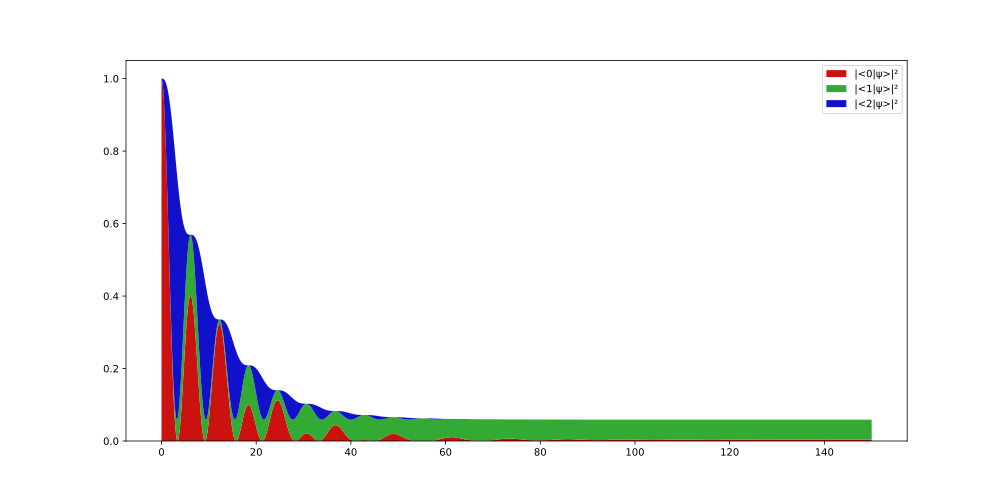
\includegraphics[width=.8\textwidth]{img/3ldetect/loss3color.pdf}
    \subcaption{Foo.}%\label{fig:aabsorbed-qubit-components_pwlattice:re0}
  \end{subfigure}
  \par\bigskip
  \par\bigskip
  \begin{subfigure}[b]{\textwidth}
    \centering
    \includegraphics[width=.8\textwidth]{img/3ldetect/loss.pdf}
    \subcaption{Bar.}%\label{fig:aabsorbed-qubit-components_pwlattice:im1}
  \end{subfigure}
  \par\bigskip
  \par\bigskip
  \caption{
    Blah blah blah.
  }
  %\label{fig:aabsorbed-qubit-components_pwlattice}
\end{figure}

% extended time

\begin{figure}[h]
  \begin{subfigure}[b]{\textwidth}
    \centering
    \includegraphics[width=\textwidth]{img/3ldetect/loss3color_ext.pdf}
    \subcaption{Foo.}%\label{fig:aabsorbed-qubit-components_pwlattice:re0}
  \end{subfigure}
  \par\bigskip
  \par\bigskip
  \begin{subfigure}[b]{\textwidth}
    \centering
    \includegraphics[width=\textwidth]{img/3ldetect/loss_ext.pdf}
    \subcaption{Bar.}%\label{fig:aabsorbed-qubit-components_pwlattice:im1}
  \end{subfigure}
  \par\bigskip
  \par\bigskip
  \caption{
    Blah blah blah.
  }
  %\label{fig:aabsorbed-qubit-components_pwlattice}
\end{figure}

% "3D"

\begin{figure}[h]
  \begin{subfigure}[b]{\textwidth}
    \centering
    \includegraphics[height=0.41\textheight,clip,trim=0 90 40 140]{img/3ldetect/NonHermitianSpaceTime_side.pdf}
    \caption{Foo.}
  \end{subfigure}
  \par\bigskip
  \begin{subfigure}[b]{\textwidth}
    \centering
    \includegraphics[height=0.44\textheight,clip,trim= 0 90 20 75]{img/3ldetect/NonHermitianSpaceTime_top.pdf}
    \caption{Bar.}
  \end{subfigure}
  \caption{FooBar.}
  %\label{fig:psi_V}
\end{figure}

% P-W

\begin{figure}[h]
  \begin{subfigure}[b]{\textwidth}
    \centering
    \includegraphics[height=0.41\textheight,clip,trim=0 90 0 140]{img/3ldetect/PWSpaceTime_side.pdf}
    \caption{Foo.}
  \end{subfigure}
  \par\bigskip
  \begin{subfigure}[b]{\textwidth}
    \centering
    \includegraphics[height=0.48\textheight,clip,trim= 0 60 0 100]{img/3ldetect/PWSpaceTime_top.pdf}
    \caption{Bar.}
  \end{subfigure}
  \caption{FooBar.}
  %\label{fig:psi_V}
\end{figure}

% P-W vs QM


\begin{figure}[h!]
  \cleardoublepage
  \centering
  \begin{subfigure}{\textwidth}
      \includegraphics[width=\textwidth]{img/3ldetect/PWSpaceTimeFit_side.pdf}
      \subcaption{Foo.}
      %\label{fig:arm1}
  \end{subfigure}
  \caption{Foobar.}
\end{figure}
\begin{figure}\ContinuedFloat
  \centering
  \begin{subfigure}{\textwidth}
      \includegraphics[width=\textwidth]{img/3ldetect/PWSpaceTimeFit_top.pdf}
      \subcaption{Bar.}
      %\label{fig:arm3}
  \end{subfigure}
  \caption{Foobar (cont.)}
\end{figure}

% P-W (bayesian) vs Detector model (norm. loss, Allcock...) detection probability

\begin{figure}[h!]
  \centering
  \includegraphics[width=\textwidth]{img/3ldetect/conditionalProbFit.pdf}
  \caption{Foo.}
  %\label{fig:psi_V}
\end{figure}

\chapter{Conclusions and Outlook}\label{ch:outlook}
\section{Discussion}

The present work has illustrated,
mainly through numerical examples
at various degrees of complexity,
and developing from existing theoretical work,
how time can be trated as a quantum observable
(described by a self-adjoint operator).

The Pauli objection (presented in Sec. \ref{proof})
is overcome because the time operator $\hat{T}$
is defined in a different Hilbert space (that we name $\hilb{H}_T$)
than the space, say $\hilb{H}_S$, where the Hamiltonian is defined,
according to the Page and Wootters model
\parencite{PageWootters, Lloyd:Time, Marletto:Evolution, Maccone:QMOT, Maccone:Pauli}.

One can introduce an extra Hilbert space, to that of ordinary quantum mechanics,
in which the time operator is defined.
\section{Relativistic formulation: Klein-Gordon}

The Klein-Gordon equation is the relativistic extension of the
(\emph{square of}) a wave equation for a free spinless particle.
Indeed, both sides have the dimension of
the square of an energy, and finding their square root
(in the operator sense) is non trivial task which was only resolved 
with the Dirac equation, from which the
intrinsic \term{spin} (particularly spin $\hbar/2$) logically emerges,
rather then being artificially introduced in the theory
to comply with the phenomenology
(\cite{Greiner_Rel}, \cite[Ch. 8]{Sakurai2}, \cite{DiracEquation}, \cite[handout 2]{Webber_notes}).

Both equations did not have much fortune as first-quantized equations,
for conceptual difficulties and historical reasons, including the rise
of Quantum Field Theory and second quantization. They do have a fundamental
role though as field equations (before quantization methods are enacted).
\parencite{PeskinSchroeder}.

The purpose of the present work is, in a sense, promoting time to a quantum
observable, or formally to a linear, self-adjoint operator in some Hilbert space.
The passage from quantum mechanics to field theory does not represent any progress
towards such goal, in that not only it does not ``promote'' time to an operator $\hat{t}$,
but it also ``demotes'' the three position operators $\hat{x}$, $\hat{y}$ and $\hat{z}$
to mere (classical) \emph{parameters}. However, consistently to relativistic covariance,
time and space coordinates are treated on equal footing. The Page and Wootters model
offers the opportunity to do the same, but both time and position are operators!

\subsection{Page and Wootters squared}

From the \eqref{eq:pwHamiltonian} and \eqref{eq:Wheeler-DeWitt}:
\begin{equation}\label{eq:pw_to_be_squared}
  -\hbar\hat{\Omega}\ox\idop_S \dket{\Psi} = \idop_T\ox\hat{H}_S \dket{\Psi} \,\text{.}
\end{equation}
Squaring the operators on both sides, we have:
\begin{equation}\label{eq:pw_squared}
  \hbar^{2}\hat{\Omega}^{2}\ox\idop_S \, \dket{\Psi} = \idop_T\ox\hat{H}_S^{2} \,\, \dket{\Psi} 
    = \idop_T \ox \left( \hat{p}^2 c^2 + m_0^2 c^4 \right) \dket{\Psi} \,\text{,}
\end{equation}
where the last equality is due to the ``quantization'' of the relation $E^2 = p^2 c^2 + m_0^2 c^4$
into $\hat{H}_S^{2} = \hat{p}^2 c^2 + m_0^2 c^4$.

We know from previous sections that in the $\qty{\ket{t}}_T$ basis $\hat{\Omega}$ is represented as
$-i\hbar\pdv{t}$. We know from standard quantum mechanics that in the $\qty{\ket{x}\ket{y}\ket{z}}_S$
basis is $\hat{p} \repr -i\hbar\nabla$. Therefore in the product basis the \eqref{eq:pw_squared} yields:
\begin{equation}\label{eq:proto_kg}
  -\hbar^2\pdv[2]{t}\Psi = \qty(-\hbar^2 c^2 \nabla^2 + m_0^2 c^4)\Psi
\end{equation}
which, up to some elementary algebra, is the well known \term{Klein-Gordon equation}.

In standard quantum mechanics (first quantization, relativistic or not)
\begin{equation}
  \ket{\psi(t)} = \int \dd{x}\dd{y}\dd{z} \Psi(x,y,z;t) \ket{x}\ox\ket{y}\ox\ket{z} \,\text{.}
\end{equation}
In this formulation
\begin{equation}
  \dket{\Psi} = \int \dd{x}\dd{y}\dd{z}\dd{t} \Psi(x,y,z,t) \ket{x}\ox\ket{y}\ox\ket{z}\ox\ket{t} \,\text{,}
\end{equation}
and $t$ is no longer a classical parameter, but an eigenvalue of the time operator,
or a label for time basis elements. Please note that, as a function of four variables,
$\Psi$ is not normalizable i.e. it's not a proper element of
$\mathcal{L}^2(\mathbb{R}^4)$
(normalization issues are tackled in \cite[eq. 23 and following]{Lloyd:Time}).

\subsection{Covariant notation}

The \eqref{eq:proto_kg} can be rearranged and expressed in explicitly covariant form:
\begin{equation}
  \qty[\partial_{\mu}\partial^{\mu} + \qty(\frac{mc}{\hbar})^2]\Psi = 0
\end{equation}
with standard relativistic notation.
Similarly
---at operator level, in the tensor product space---
the \eqref{eq:pw_squared} can be rearranged:
\begin{equation}\label{eq:pwkg}
  \qty[- \hat{\mathrm{P}}_{\mu} \hat{\mathrm{P}}^{\mu} + \qty(\frac{mc}{\hbar})^2]\Psi = 0
\end{equation}
with
\begin{equation}
\begin{aligned}\label{eq:p0123}
  \hat{\mathrm{P}}_0 &=& \frac{\hbar\hat{\Omega}}{c}  \ox \idop_x   \ox \idop_y   \ox \idop_z \\
  \hat{\mathrm{P}}_1 &=& \idop_T                      \ox \hat{p}_x \ox \idop_y   \ox \idop_z \\
  \hat{\mathrm{P}}_2 &=& \idop_T                      \ox \idop_x   \ox \hat{p}_y \ox \idop_z \\
  \hat{\mathrm{P}}_3 &=& \idop_T                      \ox \idop_x   \ox \idop_y   \ox \hat{p}_z
\end{aligned}
\end{equation}
and the usual relation between contravariant and covariant 4-vectors:
\begin{equation}
  a_\mu = \eta_{\nu}^{\mu} a^{\nu} \text{;} \quad
  \eta = \mathrm{diag}(+1, -1, -1, -1)
  \text{.}
\end{equation}

It's tempting to name the \eqref{eq:pwkg} and \eqref{eq:p0123} the \term{Page--Wootters-Klein-Gordon}
equation.\footnote{
  Or \term{Klein-Gordon-Wheeler-DeWitt-Page--Wootters-Giovannetti-Lloyd-Maccone}
  equation, thus giving
  credits to all authors, particularly if we consider that the idea of an extra Hilbert space
  was conceived originally in \cite{Lloyd:Time}.
}

As anticipated, this resolves the asymmetry in Tables \ref{op_comparison_alg} and \ref{op_comparison_J},
whereas we can write
{
  \begin{table}[h!]
    \centering
    \begin{tabular}{p{0.3\linewidth}||c|c|c}
                                                                                &
        $\hilb{H}_T$                                                            &
        $\hilb{H}_S$                                                            &
        {\footnotesize Mass term}                                               \\
      \hline
      \hline
        {\footnotesize Spatio-temporal ``positions''}                           &
        $\hat{t}$                                                               &
        $\hat{x}$                                                               &
                                                                                \\
      \hline
        {\footnotesize Canonically conjugate}                                   &
        $\hat{P_0} = \frac{\hbar\hat{\Omega}}{c} \repr -i\partial_{0}$          &
        $\hat{P}_{1,2,3} \repr -i\nabla$                                        &
                                                                                \\
      \hline
        {\footnotesize Dynamics (terms in the Wheeler-DeWitt equation)}         &
        $\hat{P}_{0}\hat{P}^{0} \repr -\hbar^2 \partial_{0}\partial^{0}$        &
        $\hat{P}_{j}\hat{P}^{j} \repr -\hbar^2 \partial_{j}\partial^{j}$        &
        $\qty(\frac{mc}{\hbar})^2$
    \end{tabular}
    \caption{
      Operators in the space-time Hilbert spaces.
    }
  \end{table}
}
\section{Other topics}\label{sec:outlook-misc}

\subsection{Quantum computing and decomposition}

In Sec.~\ref{sec:finite-quantum}, it was noted that
``a benefit of finite-dimensional systems is the potential implementation on a finite array of
qubits in a quantum computer''.
Indeed,
experimentally,
besides looking for a suitable $N$-level system to act as a clock,
we may want to ``encode'' $2^{n}$ levels into the combined state of $n$
qubits and
decompose $\mathbb{J}$ (or, actually, $e^{-i\mathbb{J}\tau/\hbar}$)
into simpler hamiltonians (respectively: evolutions)
acting on individual qubits (\term{gates}),
therefore allowing the experiment to be run on a quantum processor.
A decomposition method that can be considered for the purpose
is the Trotter-Suzuki scheme
\parencite{Trotter-Suzuki:exp, Trotter-Suzuki:GPU}.

\subsection{Time crystals}

References: \cite{crystal3,crystal2012}.


\subsection{Quantifying entanglement}

Vedral: \url{https://arxiv.org/abs/quant-ph/9702027}.

Jon Yard, entropy: \href{http://www.perimeterinstitute.ca/fr/videos/quantifying-entanglement-quantum-entropy}{Perimeter video}.

Caterina-Eloisa Mora, ``beyond'':
\href{https://www.perimeterinstitute.ca/videos/quantifying-quantumness-correlations-beyond-entanglement-and-back}{Perimeter video},
\href{https://arxiv.org/search/advanced?advanced=&terms-0-operator=AND&terms-0-term=Mora%2C+caterina-eloisa&terms-0-field=author&terms-1-operator=OR&terms-1-term=mora%2C+c+e&terms-1-field=author&classification-physics_archives=all&classification-include_cross_list=include&date-filter_by=all_dates&date-year=&date-from_date=&date-to_date=&date-date_type=submitted_date&abstracts=show&size=50&order=-announced_date_first}{arXiv search}.

Geometric measure: \url{https://arxiv.org/abs/quant-ph/0307219}.

``Resources'': \url{https://arxiv.org/abs/1402.6710}.

\section{Entanglement and decoherence (Arrow of time)}
See also \cite{EntanglementVsDecoherence}.

Decoherence is an irreversible process, it also happens in measurement.

According to Marletto and Vedral, arrow of time is increase in Entanglement
between the clock and the rest.

So, there seems to be a contradiction: is entanglement ``decreasing''
(i.e. destroyed by decoherence) with time
or increasing?

We can avoid the contradiction saying that
entanglement between two finite systems is
destroyed while the entanglement of each of them with the universe
is increasing.

\subsection{``Harmonic clocks''}

Use the harmonic oscillator in \cite{HarmonicClocks}
as a PaW clock for the same packet that is measured in
Ruschhaupt's detector model.

Therein, fading wave function: is minus derivative an event?
L4 normalized?

\subsection{Atomic clocks / quantum clocks}
Technologically implemented! There is a section in the intro chapter of the book,
\emph{and} a dedicated chapter.

\subsection{Misc}

Idea: use section B ``Measurement'' of \cite{Lloyd:Time}: detector as (binary) measument device.

``Philospher'': \url{https://arxiv.org/abs/1704.07236}.

Time of arrival and clocks: again, \cite{YearsleyHalliwell_Clocks}.
Which maybe suggests we should not worry too much of $H\ket{\Psi} = 0$.

We don't.

BUT please note \cite{YearsleyHalliwell_Clocks} uses a clock that is
\emph{coupled} with the system, while in PaW they are ``only'' entangled.
So their calculation may be unnecessarily complicated.
Maybe the weakjly coupling case can be used?

Other systems of interest: decays. Prvanovic new.

Reference \cite{ConnesRovelliThermo}.

Relate with John Goold's works? The ancilla as a clock? --- Topical Review

Markovianity, histories.

Lloyd on arXiv: from clock to cloners; erasing; scrambling (as in Goold).

Lloyd on decoherent histories (Gellman, Hartle?).

Dechoerence / irreversibility / measurement.

Vedral / Lloyd. Discord.

Measuring entanglement: Quantification of Concurrence via Weak Measurement: 1611.00149.

Marletto/Vedral on Arrow of time. Arrow of time as increasing entanglement.

Arrow of time:

\url{https://www.wired.com/2014/04/quantum-theory-flow-time/}

\url{https://en.wikipedia.org/wiki/Loschmidt%27s_paradox}

\url{https://www.quantamagazine.org/20160119-time-entanglement/}

\url{https://arxiv.org/pdf/1702.07706.pdf} \textit{The second law of thermodynamics at the microscopic scale}
Thibaut Josset,
Aix Marseille Univ. (David).

Maxwell's demon: https://arxiv.org/pdf/1702.05161.pdf

\subsection{and paths}

Both \cite{YearsleyHalliwell_Clocks} and \cite{Gambini_PW}
reason in terms of paths and actions, maybe Feynmann stuff
in following chapter... and maybe conistent historiesapproach can help
towards linking PaW and ToA?

Also \url{http://quantum.phys.cmu.edu/CHS/CHS_transp.pdf}.

\subsection{Decays?}

We might want to look at exponential decay from \url{https://arxiv.org/abs/1704.07236},
then compare with exponential decay with P and W using Lloyd Giovannetti and Maccone (ref).

\subsubsection{Purification}

See https://arxiv.org/pdf/quant-ph/0512125.pdf, P-W time as a purifying ancilla
of the (Kijowski?) time.

\section{Misc/Multi/Extras/Outlook}

\url{https://arxiv.org/abs/1703.05876}
--- \emph{comment}: time measured and stored here
may be all classical information
so this paper may or may not be relevant for the topic.

But
``prototypes of clocks based on quantum principles,
such as entanglement and squeezing''
may make this interesting again, see reference therein.
They also cite Lloyd, Giovannetti and Maccone,
but a paper quite older than \cite{Lloyd:Time}.

\url{https://arxiv.org/abs/1603.02522}
\emph{Decoherence by spontaneous emission: a single-atom analog of superradiance}.
Decoherent histories, non-markovianity, open quantum systems.

\url{https://arxiv.org/abs/1007.2615} Time travel / Quantum CTC.

Carmichael et al. \cite{CarmichaelOQS2017} (Andreas's reading)
(non-markovianity).

Non-markovian, quantum-to-classical, open systems, David,
\url{https://arxiv.org/pdf/1703.09428.pdf}.

In his works, Zurek mentions:
DeWitt, Everett, gell_Mann, hartl, Many Worlds, consistent/decoherent histories:
idea: Lagrangian over a history? Principle of least action?

Zurek: ``Reduction of the Wavepacket: How Long Does it Take?'' (arxiv),
``quantum''' time? \cite{Zurek_Einselect} also mentions
``decoherence timescale''.

Von Neumann/Shannon entropy in measurement? Mention information problems
in quantum cosmology (where a quantum time is necessary)? Etc. etc.

\section{for Relativistic treatment}

Lorentz (+Galilei?) transformation. Lorent/Poincare groups. May be Important:
see \cite{LocalizationEntanglmentRelativistic}.

\cite{Misra}? Cited in TQM book 1 chap. 1 as 
``a different way out in the context of a theory of irreversible evolution''.
Mentions Klein-Gordon and Poincare group.

\cite{RealisticClocks}.

\cite{HarmonicClocks} concludes ``Classical clock can be described by an Hamiltonian linear in momentum''\dots
like in relativity?

\cite{Lloyd:Time} does not only deal with improper eigenstates in $\hilb{H}_T$
(full evolutions?)
but also normalized ones (in $\hilb{H}_T$! \emph{``Events''}?)

A Page and Wootters time of arrival is mentioned in \cite{Gambini_PW}.

\subsection{Time-of-arrival for a Klein-Gordon free particle}

See \cite{Galapon_KG}.

\subsection{Dirac eq.}

\url{https://arxiv.org/pdf/1502.00322.pdf}



\subsection{Feynmann path stuff}

Sokolovski 1703.01966, Feynmann paths...\subsection{(dis)entanglement under gravity, decoherence, event formalism}

1703.08036 An experiment to test decoherence under gravity aka entangled photons undergoing different paths and how their entanglement is affected.
``Space QUEST mission proposal: Experimentally testing decoherence due to gravity''.

Are they getting entangled with the environment instead? (Merletto and Vedral).

The theoretical paper behind the space experiment: \url{https://arxiv.org/pdf/1406.3677.pdf}. Interestingly, it mentions 
\emph{event formalism}, and we thought about that: is an event something
representable as a proper vector in $\mathscr{L}^2(\mathbb{R}^4)$ --- where one of the dimensions is time?
Deepen the event formalism if it's quantum.

Resume ``Quantum Statistical Gravity''? \url{https://arxiv.org/abs/1602.05707}.

``Fundamental decoherence from quantum gravity: a pedagogical review''
\url{https://arxiv.org/abs/gr-qc/0603090} ---
``fundamental loss of unitarity
that appears in quantum mechanics
due to the use of a physical apparatus to measure time''.

Closed timelike curves are also the subject of a paper by Lloyd (cite!).

``Deutsch argued that
the usual paradoxes associated with such solutions of general
relativity can be resolved by quantum mechanics''  in the reference above. But in the even formalism
\emph{spacetime is still a classical background!}. Event operators a parametrized by $t$\dots

\subsection{Prvanovic and P\&W}
In \cite{Prvanovic}, essentially the clock observable is the Hamiltonian.
The two example clocks are an harmonic oscillator and a free particle.
The harmonic oscillator features discrete time. Generally a time which is
{bounded from below}
is consistent with the Big Bang...

Prvanovic uses ``relativisitc'' constants...

BTW, please note a time bounded from below WOULD NOT be sufficient to overcome the Pauli objection alone.

\section{Photon position}

Quantum mechanics is a 0+1 QFT \parencite{QFT_0+1}.
The \emph{dimension} of the field theory is the number of external parameters.
The P-W mechanism ``quantizes'' external parameters, or make their property
of classical external parameter \emph{emerge} out of a quantum observable
of an entangled subsystem (where there exists a Schmidt decomposition over
eigenstates of said observable).

In this sense, time in quantum mechanics is like time \emph{and position}
in quantum field theories such as quantum optics or the Standard Model.

We can imagine P-W ``meter sticks'' instead of clocks, to measure
photon position and thus tackle the same problem of \cite{HawtonPhotonPosition}.

\section{Photon \emph{absorption}}

Photons are physically/really absorbed (or \emph{emitted}), although under a different theoretical framework
(second quantized Vs QM). No need of complex potentials\dots Connect with spontaneous emission?

Spontaneous emission/decay compared with PW (Maccone) and Kiukas (detection).
Perhaps Prvanovic article on spontaneous decay?


% appendices
\appendix

\chapter[Jupyter Notebooks]{Jupyter Notebooks\footnote{
  For a reference on the software tools utilized:
  \cite{comp:scipy};
  \cite{comp:sympy};
  \cite{comp:jupyter};
  \cite{comp:matplotlib};
  \cite{comp:numpy}.
}}
\section*{Technical note}

Original files available at
the code repository, ref. \cite{OwnJupyterRepo}.

Printable and embeddable \TeX{} files have been generated with
\begin{itemize}
  \item
    ``Download as Markdown'' from Jupyter user interface
  \item
    Installing and running \verb#pandoc#\footnote{ \url{http://pandoc.org/}}
    on the generated \verb#.md# file\footnote{ See also \url{https://tex.stackexchange.com/a/314785}.}
    \begin{lstlisting}[language=Bash]
      pandoc --listings -f markdown -t latex myfile.md -o myfile.tex
    \end{lstlisting}
  \item
    Tweaking generated \verb#\label#'s and other references as needed to avoid inconsistencies and overlaps
\end{itemize}

\hypertarget{analysys-of-the-moreva-et-al.experiment}{%
\section{Analysys of the Moreva et
al.~experiment}\label{analysys-of-the-moreva-et-al.experiment}}

\hypertarget{preliminaries}{%
\subsection{Preliminaries}\label{preliminaries}}

\begin{lstlisting}[language=Python]
# Symbolic computation
from sympy import *
from sympy.physics.matrices import mdft
from sympy.physics.quantum import TensorProduct
from sympy.physics.quantum.constants import hbar
\end{lstlisting}

\begin{lstlisting}[language=Python]
# Remeber this to have LaTeX rendered output in Jupyter
init_printing()
\end{lstlisting}

\hypertarget{computation}{%
\subsection{Computation}\label{computation}}

\begin{lstlisting}[language=Python]
Omega = Symbol(r'\Omega')
omega = Symbol(r'\omega', real=True)
\end{lstlisting}

\begin{lstlisting}[language=Python]
F = mdft(2)
\end{lstlisting}

\begin{lstlisting}[language=Python]
Omega = I*omega*Matrix([
    [0, 1],
    [-1,0]
])
\end{lstlisting}

\begin{lstlisting}[language=Python]
Omega.eigenvects()
\end{lstlisting}

\[\left [ \left ( - \omega, \quad 1, \quad \left [ \left[\begin{matrix}- i\\1\end{matrix}\right]\right ]\right ), \quad \left ( \omega, \quad 1, \quad \left [ \left[\begin{matrix}i\\1\end{matrix}\right]\right ]\right )\right ]\]

\begin{lstlisting}[language=Python]
T = (pi / (2*omega)**2) * F.adjoint()*Omega*F
\end{lstlisting}

\begin{lstlisting}[language=Python]
T
\end{lstlisting}

\[\left[\begin{matrix}0 & - \frac{i \pi}{4 \omega}\\\frac{i \pi}{4 \omega} & 0\end{matrix}\right]\]

\begin{lstlisting}[language=Python]
T.eigenvects()
\end{lstlisting}

\[\left [ \left ( - \frac{\pi}{4 \omega}, \quad 1, \quad \left [ \left[\begin{matrix}i\\1\end{matrix}\right]\right ]\right ), \quad \left ( \frac{\pi}{4 \omega}, \quad 1, \quad \left [ \left[\begin{matrix}- i\\1\end{matrix}\right]\right ]\right )\right ]\]

\begin{lstlisting}[language=Python]
T_d = diag(-pi/(4*omega), pi/(4*omega))
\end{lstlisting}

\begin{lstlisting}[language=Python]
T_d
\end{lstlisting}

\[\left[\begin{matrix}- \frac{\pi}{4 \omega} & 0\\0 & \frac{\pi}{4 \omega}\end{matrix}\right]\]

Check: this is what we would obtain with matric of cols egeinv

\begin{lstlisting}[language=Python]
R = (1/sqrt(2)) * Matrix([
    [I, -I],
    [1, 1]
])
\end{lstlisting}

\begin{lstlisting}[language=Python]
R.adjoint()*T*R
\end{lstlisting}

\[\left[\begin{matrix}- \frac{\pi}{4 \omega} & 0\\0 & \frac{\pi}{4 \omega}\end{matrix}\right]\]

\begin{lstlisting}[language=Python]
Omega_T_d = (pi/((pi/(2*omega))**2))*F*T_d*F.adjoint()
\end{lstlisting}

\begin{lstlisting}[language=Python]
Omega_T_d
\end{lstlisting}

\[\left[\begin{matrix}0 & - \omega\\- \omega & 0\end{matrix}\right]\]

\begin{lstlisting}[language=Python]
Hs = I*hbar*omega*Matrix([
    [0, 1],
    [-1,0]
])
\end{lstlisting}

\begin{lstlisting}[language=Python]
J = TensorProduct(hbar*Omega_T_d, eye(2)) + TensorProduct(eye(2), Hs)
\end{lstlisting}

\begin{lstlisting}[language=Python]
J
\end{lstlisting}

\[\left[\begin{matrix}0 & \hbar i \omega & - \hbar \omega & 0\\- \hbar i \omega & 0 & 0 & - \hbar \omega\\- \hbar \omega & 0 & 0 & \hbar i \omega\\0 & - \hbar \omega & - \hbar i \omega & 0\end{matrix}\right]\]

\begin{lstlisting}[language=Python]
J.eigenvects()
\end{lstlisting}

\[\left [ \left ( 0, \quad 2, \quad \left [ \left[\begin{matrix}0\\- i\\1\\0\end{matrix}\right], \quad \left[\begin{matrix}i\\0\\0\\1\end{matrix}\right]\right ]\right ), \quad \left ( - 2 \hbar \omega, \quad 1, \quad \left [ \left[\begin{matrix}- i\\1\\- i\\1\end{matrix}\right]\right ]\right ), \quad \left ( 2 \hbar \omega, \quad 1, \quad \left [ \left[\begin{matrix}- i\\-1\\i\\1\end{matrix}\right]\right ]\right )\right ]\]

\hypertarget{ordinary-quantum-theory}{%
\subsection{Ordinary quantum theory}\label{ordinary-quantum-theory}}

\begin{lstlisting}[language=Python]
t = Symbol('t')
t0 = Symbol('t_0')
\end{lstlisting}

\begin{lstlisting}[language=Python]
exp(-I*Hs*(t-t0)/hbar)
\end{lstlisting}

\[\left[\begin{matrix}\frac{1}{2} e^{i \omega \left(t - t_{0}\right)} + \frac{1}{2} e^{- i \omega \left(t - t_{0}\right)} & - \frac{i}{2} e^{i \omega \left(t - t_{0}\right)} + \frac{i}{2} e^{- i \omega \left(t - t_{0}\right)}\\\frac{i}{2} e^{i \omega \left(t - t_{0}\right)} - \frac{i}{2} e^{- i \omega \left(t - t_{0}\right)} & \frac{1}{2} e^{i \omega \left(t - t_{0}\right)} + \frac{1}{2} e^{- i \omega \left(t - t_{0}\right)}\end{matrix}\right]\]

\begin{lstlisting}[language=Python]
exp(-I*Hs*(t-t0)/hbar) * Matrix([0, -I])
\end{lstlisting}

\[\left[\begin{matrix}- i \left(- \frac{i}{2} e^{i \omega \left(t - t_{0}\right)} + \frac{i}{2} e^{- i \omega \left(t - t_{0}\right)}\right)\\- i \left(\frac{1}{2} e^{i \omega \left(t - t_{0}\right)} + \frac{1}{2} e^{- i \omega \left(t - t_{0}\right)}\right)\end{matrix}\right]\]

\begin{lstlisting}[language=Python]
(exp(-I*Hs*(t-t0)/hbar) * Matrix([0, -I])).subs({t: pi/(4*omega), t0: -pi/(4*omega)})
\end{lstlisting}

\[\left[\begin{matrix}- i\\0\end{matrix}\right]\]

There is consistency in predicting the probability (square modulus), but
not probability amplitute: at \(t=\frac{\pi}{4\omega}\) P-W finds
\((1, 0)\) instead of \((-i, 0)\). But the Rabi oscillation in terms of
probability from 100\% \(\left|V\right>\) at
\(t=t_0=-\frac{\pi}{4\omega}\), to 100\% \(\left|H\right>\) at
\(t=\frac{\pi}{4\omega}\) is correctly predicted.

\hypertarget{nb:moreva-vs-qm}{%
\section{Comparison with ordinary
QM, with phase correction and plotting}\label{nb:moreva-vs-qm}}

Conversions from symbolic to numeric (including implicit one) for
plotting seems problematic, either with \verb#subs()#
or \verb#lambdify()#, therefore we start over, with a
new notebook. We also assume \begin{equation*}
    \hbar = \omega = 1 \,\text{.}
\end{equation*}

\begin{lstlisting}[language=Python]
import numpy as np
from scipy.linalg import expm
\end{lstlisting}

\begin{lstlisting}[language=Python]
import matplotlib as mpl
from mpl_toolkits.mplot3d import Axes3D
import numpy as np
import matplotlib.pyplot as plt
\end{lstlisting}

\begin{lstlisting}[language=Python]
%matplotlib inline
\end{lstlisting}

\begin{lstlisting}[language=Python]
Hs = np.array([
    [0, 1j],
    [-1j, 0]
])
\end{lstlisting}

\begin{lstlisting}[language=Python]
def evolve_psi(t, t0, psi0):
    return expm(-1j*Hs*(t-t0)).dot(psi0)
\end{lstlisting}

\begin{lstlisting}[language=Python]
def correction_eigenJ(-t, t0, eigenvalue):
    return np.exp(1j*eigenvalue*(t-t0))
\end{lstlisting}

\begin{lstlisting}[language=Python]
def correction_timeshift(t, t0, timeshift):
    deltaT = np.pi/2
    omega_prime = (np.pi*timeshift) / (deltaT**2)
    return np.exp(-1j*omega_prime*(t-t0))
\end{lstlisting}

\begin{lstlisting}[language=Python]
def psi_fixed(t, t0, psi0, eigenvalue):
    return evolve_psi(t, t0, psi0) * correction_eigenJ(t, t0, eigenvalue) * correction_timeshift(t, t0, t0)
\end{lstlisting}

\begin{lstlisting}[language=Python]
def psi_fixed_0_re(t, t0, psi0, eigenvalue):
    return np.real(psi_fixed(t, t0, psi0, eigenvalue)[0])
\end{lstlisting}

\begin{lstlisting}[language=Python]
def psi_fixed_0_im(t, t0, psi0, eigenvalue):
    return np.imag(psi_fixed(t, t0, psi0, eigenvalue)[0])
\end{lstlisting}

\begin{lstlisting}[language=Python]
def psi_fixed_1_re(t, t0, psi0, eigenvalue):
    return np.real(psi_fixed(t, t0, psi0, eigenvalue)[1])
\end{lstlisting}

\begin{lstlisting}[language=Python]
def psi_fixed_1_im(t, t0, psi0, eigenvalue):
    return np.imag(psi_fixed(t, t0, psi0, eigenvalue)[1])
\end{lstlisting}

\begin{lstlisting}[language=Python]
mpl.rcParams['legend.fontsize'] = 10

fig = plt.figure(figsize=(15, 11))
ax = fig.gca(projection='3d')

# Prepare arrays x, y, z
# z is t
z = np.linspace(-np.pi/4, 3*np.pi/4, 500)

# Auto-broadcasting doesn't work as expected, therefore we explicitly
# map the z vector via `np.vectorize()`

# x is real part of psi[0] or Re(psi_H) as in psi = psi_H|H> + psi_V|V>
x = np.vectorize(lambda t: psi_fixed_0_re(t, -np.pi/4, [0, -1j], 0))(z) 
# y is imag part of psi[0] or Im(psi_H) as in psi = psi_H|H> + psi_V|V>
y = np.vectorize(lambda t: psi_fixed_0_im(t, -np.pi/4, [0, -1j], 0))(z) 

plt.plot([0, 0], [0, 0], [-np.pi/4, 3*np.pi/4], lw=1, c='pink', label='Time (clock cycle)')

ax.plot(x, y, z, label='\psi_H "rephased"')

points_x = np.array([     0.0,     1.0,       0.0])
points_y = np.array([     0.0,     0.0,       0.0])
points_z = np.array([-np.pi/4, np.pi/4, 3*np.pi/4])
ax.scatter(points_x, points_y, points_z, marker='^', c='red', s=50, alpha=1.0, label='discrete PW')

plt.xlabel(s='Re <H|psi>')
plt.ylabel(s='Im <H|psi>')
ax.set_zlabel('t')

ax.legend()

plt.show()
\end{lstlisting}

\begin{figure}
\centering
\includegraphics[width=\textwidth/2]{img/psi_H.png}
\caption[]{png}{png}
\end{figure}

\begin{lstlisting}[language=Python]
mpl.rcParams['legend.fontsize'] = 10

fig = plt.figure(figsize=(15, 11))
ax = fig.gca(projection='3d')

# Prepare arrays x, y, z
# z is t
z = np.linspace(-np.pi/4, 3*np.pi/4, 500)

# Auto-broadcasting doesn't work as expected, therefore we explicitly
# map the z vector via `np.vectorize()`

# x is real part of psi[1] or Re(psi_V) as in psi = psi_H|H> + psi_V|V>
x = np.vectorize(lambda t: psi_fixed_1_re(t, -np.pi/4, [0, -1j], 0))(z) 
# y is imag part of psi[0] or Im(psi_H) as in psi = psi_H|H> + ps_V|V>
y = np.vectorize(lambda t: psi_fixed_1_im(t, -np.pi/4, [0, -1j], 0))(z) 

plt.plot([0, 0], [0, 0], [-np.pi/4, 3*np.pi/4], lw=1, c='pink', label='Time (clock cycle)')

ax.plot(x, y, z, label='psi_V "rephased"')

points_x = np.array([     0.0,     0.0,       0.0])
points_y = np.array([    -1.0,     0.0,      -1.0])
points_z = np.array([-np.pi/4, np.pi/4, 3*np.pi/4])
ax.scatter(points_x, points_y, points_z, marker='^', c='red', s=50, alpha=1.0, label='discrete PW')

plt.xlabel(s='Re <V|psi>')
plt.ylabel(s='Im <V|psi>')
ax.set_zlabel('t')

ax.legend()

plt.show()
\end{lstlisting}

\begin{figure}
\centering
\includegraphics[width=\textwidth/2]{img/psi_V.png}
\caption[]{png}{png}
\end{figure}

\graphicspath{{tex/appendix/nb/jupyter/detect/}}

\hypertarget{detector-model-kiukas-ruschhaupt-schmidt-werner}{%
\section[Detector model: Kiukas, Ruschhaupt, Schmidt, Werner]{Detector model: Kiukas, Ruschhaupt, \linebreak[4] Schmidt, Werner}
\label{detector-model-kiukas-ruschhaupt-schmidt-werner}}

\begin{lstlisting}[language=Python]
from sympy import *
#from sympy.physics.matrices import mdft
from sympy.physics.quantum import TensorProduct
from sympy.functions.special.delta_functions import Heaviside
from sympy.physics.quantum.dagger import Dagger

from sympy.stats import ContinuousRV, variance, std

from sympy.plotting import plot, plot3d_parametric_line

import numpy as np
import matplotlib
import matplotlib.pyplot as plt

matplotlib.rcParams['text.usetex'] = True
#matplotlib.rcParams['text.latex.preamble'] = r'''
#    \usepackage{DejaVuSans}
#    \usepackage{xparse}
#    \usepackage{amsmath}
#    \usepackage{physics}
#'''
#matplotlib.rcParams['mathtext.fontset'] = 'dejavusans' 
#matplotlib.rcParams['mathtext.default'] = 'sf'
matplotlib.rcParams['figure.dpi'] = 140
# matplotlib.rcParams['figure.figsize'] = (8,8/sqrt(2))
matplotlib.rcParams['axes.labelsize'] = 16

# https://matplotlib.org/gallery/mplot3d/lines3d.html?highlight=parametric
# This import registers the 3D projection, but is otherwise unused.
from mpl_toolkits.mplot3d import Axes3D  # noqa: F401 unused import
\end{lstlisting}

\begin{lstlisting}[language=Python]
gamma = Symbol('gamma', real=True)
t = Symbol('t', real=True)
tprime = Symbol('t\'', real=True)
omega = Symbol('omega', real=True)
nu = Symbol('nu', real=True)
\end{lstlisting}

\begin{lstlisting}[language=Python]
def D(_gamma):
    return Rational(1, 2) * Matrix([
        [0, 0],
        [0, _gamma]
    ])
\end{lstlisting}

\begin{lstlisting}[language=Python]
H = Matrix ([
[0, 1] ,
[1, 0]
])
\end{lstlisting}

\begin{lstlisting}[language=Python]
init_printing ()
\end{lstlisting}

\begin{lstlisting}[language=Python]
H
\end{lstlisting}

\[\left[\begin{matrix}0 & 1\\1 & 0\end{matrix}\right]\]

\begin{lstlisting}[language=Python]
H.eigenvects()
\end{lstlisting}

\[\left [ \left ( -1, \quad 1, \quad \left [ \left[\begin{matrix}-1\\1\end{matrix}\right]\right ]\right ), \quad \left ( 1, \quad 1, \quad \left [ \left[\begin{matrix}1\\1\end{matrix}\right]\right ]\right )\right ]\]

It's manually seen that \(\langle H \rangle = 0\) and
\(\langle H^2 \rangle = 1\), therefore \(\sigma_{H} = 1\).

\begin{lstlisting}[language=Python]
def K(_gamma):
    return H - I*D(_gamma)
\end{lstlisting}

\begin{lstlisting}[language=Python]
K(2*sqrt(2))
\end{lstlisting}

\[\left[\begin{matrix}0 & 1\\1 & - \sqrt{2} i\end{matrix}\right]\]

\begin{lstlisting}[language=Python]
K(2*sqrt(2)).eigenvects()
\end{lstlisting}

\[\left [ \left ( - \frac{\sqrt{2}}{2} - \frac{\sqrt{2} i}{2}, \quad 1, \quad \left [ \left[\begin{matrix}- \frac{1}{\frac{\sqrt{2}}{2} + \frac{\sqrt{2} i}{2}}\\1\end{matrix}\right]\right ]\right ), \quad \left ( \frac{\sqrt{2}}{2} - \frac{\sqrt{2} i}{2}, \quad 1, \quad \left [ \left[\begin{matrix}- \frac{1}{- \frac{\sqrt{2}}{2} + \frac{\sqrt{2} i}{2}}\\1\end{matrix}\right]\right ]\right )\right ]\]

\begin{lstlisting}[language=Python]
def B(_gamma):
    return lambda t: exp(-I*K(_gamma)*t)
\end{lstlisting}

\begin{lstlisting}[language=Python]
def U():
    return lambda t: exp(-I*H*t)
\end{lstlisting}

\begin{lstlisting}[language=Python]
def non_unitary_psi(_t):
    return B(2*sqrt(2))(_t) * Matrix([1,0])
\end{lstlisting}

\begin{lstlisting}[language=Python]
def unitary_psi(_t):
    return U()(_t) * Matrix([1,0])
\end{lstlisting}

\begin{lstlisting}[language=Python]
non_unitary_psi(t)
\end{lstlisting}

\begin{equation}\label{eq:sympy:non-unitary-evol}
    \left[\begin{matrix}\frac{\sqrt{2} i t e^{- \frac{\sqrt{2} t}{2} - \frac{\sqrt{2} i t}{2}}}{2 \left(\frac{\sqrt{2} t}{2} + \frac{\sqrt{2} i t}{2}\right)} - \frac{\sqrt{2} i t e^{- \frac{\sqrt{2} t}{2} + \frac{\sqrt{2} i t}{2}}}{2 \left(\frac{\sqrt{2} t}{2} - \frac{\sqrt{2} i t}{2}\right)}\\\frac{\sqrt{2} e^{- \frac{\sqrt{2} t}{2} - \frac{\sqrt{2} i t}{2}}}{2} - \frac{\sqrt{2} e^{- \frac{\sqrt{2} t}{2} + \frac{\sqrt{2} i t}{2}}}{2}\end{matrix}\right]
\end{equation}

New period

\begin{lstlisting}[language=Python]
2*pi / (sqrt(2)/2)
\end{lstlisting}

\[2 \sqrt{2} \pi\]

Components are either pure real or pure imaginary:

\begin{lstlisting}[language=Python]
plot(re(non_unitary_psi(t)[0]), (t, 0, 10),
     line_color='r', xlabel=r'$t$', ylabel=r'$\mathrm{Re}\left\langle 0 | \psi \right\rangle $')
\end{lstlisting}

\begin{figure}
\centering
\includegraphics[width=0.6\linewidth]{output_20_0.png}
\caption[]{png}
\end{figure}

\begin{lstlisting}
<sympy.plotting.plot.Plot at 0x7fe25ffc9898>
\end{lstlisting}

\begin{lstlisting}[language=Python]
plot(im(non_unitary_psi(t)[1]), (t, 0, 10),
     line_color='b', xlabel=r'$t$', ylabel=r'$\mathrm{Im}\left\langle 1 | \psi \right\rangle $')
\end{lstlisting}

\begin{figure}
\centering
\includegraphics[width=0.6\linewidth]{output_21_0.png}
\caption[]{png}
\end{figure}

\begin{lstlisting}
<sympy.plotting.plot.Plot at 0x7fe25fec1780>
\end{lstlisting}

\begin{lstlisting}[language=Python]
# verify that our manual simplification is correct
#plot(-sqrt(2)*exp(-t*sqrt(2)/2)*sin(t*sqrt(2)/2), (t, 0, 10) )
\end{lstlisting}

\begin{lstlisting}[language=Python]
def lossy_norm(_t):
    psi = B(2*sqrt(2))(_t) * Matrix([1,0])
    return (abs(psi[0]**2) + abs(psi[1]**2))
\end{lstlisting}

\begin{lstlisting}[language=Python]
lossy_norm(t)
\end{lstlisting}

\[\left|{\left(\frac{\sqrt{2} e^{- \frac{\sqrt{2} t}{2} - \frac{\sqrt{2} i t}{2}}}{2} - \frac{\sqrt{2} e^{- \frac{\sqrt{2} t}{2} + \frac{\sqrt{2} i t}{2}}}{2}\right)^{2}}\right| + \left|{\left(\frac{\sqrt{2} i t e^{- \frac{\sqrt{2} t}{2} - \frac{\sqrt{2} i t}{2}}}{2 \left(\frac{\sqrt{2} t}{2} + \frac{\sqrt{2} i t}{2}\right)} - \frac{\sqrt{2} i t e^{- \frac{\sqrt{2} t}{2} + \frac{\sqrt{2} i t}{2}}}{2 \left(\frac{\sqrt{2} t}{2} - \frac{\sqrt{2} i t}{2}\right)}\right)^{2}}\right|\]

\begin{lstlisting}[language=Python]
non_unitary_psi_n = lambdify(t, non_unitary_psi(t), "numpy")
\end{lstlisting}

\begin{lstlisting}[language=Python]
_lossy_norm_n = lambdify(t, lossy_norm(t), "numpy")
def lossy_norm_n(__t):
    # prevent a warning, even if we know it's real
    return np.real(_lossy_norm_n(__t))
\end{lstlisting}

\begin{lstlisting}[language=Python]
lossy_norm_n
\end{lstlisting}

\begin{lstlisting}
<function __main__.lossy_norm_n(__t)>
\end{lstlisting}

\begin{lstlisting}[language=Python]
def non_unitary_psi_renorm_n(_t):
    return non_unitary_psi_n(_t) / np.sqrt(lossy_norm_n(_t))
\end{lstlisting}

\begin{lstlisting}[language=Python]
T = np.linspace(1e-16, 2*np.pi, 2000)
\end{lstlisting}

\begin{lstlisting}[language=Python]
fig = plt.figure(figsize=(8,8))
#fig = plt.figure()


ax = fig.gca(projection='3d')
ax.view_init(10,-45) # rotate 3d point of view

ax.plot(
    np.real(non_unitary_psi_n(T)[0][0]), np.imag(non_unitary_psi_n(T)[1][0]), T,
    linewidth=1.25
)

##ax.legend()

plt.xlabel(r'$\mathrm{Re}\left\langle 0 | \psi \right\rangle$ (pure real)', labelpad=8)
plt.ylabel(r'$\mathrm{Im}\left\langle 1 | \psi \right\rangle$ (pure imag)', labelpad=10)
ax.set_zlabel(r'$t$')
\end{lstlisting}

\begin{lstlisting}
Text(0.5, 0, '$t$')
\end{lstlisting}

\begin{figure}
\centering
\includegraphics[width=0.6\linewidth]{output_30_1.png}
\caption[]{png}
\end{figure}

\begin{lstlisting}[language=Python]
plot(lossy_norm(t),(t, 0, 2*pi), line_color='g',
     ylabel=r'$\left|\psi\right|^2$', xlabel=r'$t$')
\end{lstlisting}

\begin{figure}
\centering
\includegraphics[width=0.6\linewidth]{output_31_0.png}
\caption[]{png}
\end{figure}

\begin{lstlisting}
<sympy.plotting.plot.Plot at 0x7fe25fe6a6a0>
\end{lstlisting}

\begin{lstlisting}[language=Python]
def prob_0_detect(t):
    return abs(non_unitary_psi(t)[0]**2) / lossy_norm(t)
\end{lstlisting}

\begin{lstlisting}[language=Python]
def prob_1_detect(t):
    return abs(non_unitary_psi(t)[1]**2) / lossy_norm(t)
\end{lstlisting}

\begin{lstlisting}[language=Python]
plot(prob_0_detect(t),(t, 0, 2*pi), line_color='r')
\end{lstlisting}

\begin{figure}
\centering
\includegraphics[width=0.6\linewidth]{output_34_0.png}
\caption[]{png}
\end{figure}

\begin{lstlisting}
<sympy.plotting.plot.Plot at 0x7fe25fddca20>
\end{lstlisting}

\begin{lstlisting}[language=Python]
plot(prob_1_detect(t),(t, -0, 2*pi), line_color='b')
\end{lstlisting}

\begin{figure}
\centering
\includegraphics[width=0.6\linewidth]{output_35_0.png}
\caption[]{png}
\end{figure}

\begin{lstlisting}
<sympy.plotting.plot.Plot at 0x7fe25fd87ac8>
\end{lstlisting}

\begin{lstlisting}[language=Python]
plot(re(non_unitary_psi(t)[0])/sqrt(lossy_norm(t)), (t, 0, 2 * 2*sqrt(2)*pi), line_color='r')
\end{lstlisting}

\begin{figure}
\centering
\includegraphics[width=0.6\linewidth]{output_36_0.png}
\caption[]{png}
\end{figure}

\begin{lstlisting}
<sympy.plotting.plot.Plot at 0x7fe25fd03128>
\end{lstlisting}

\begin{lstlisting}[language=Python]
plot(im(non_unitary_psi(t)[1])/sqrt(lossy_norm(t)), (t, 0, 2 * 2*sqrt(2)*pi), line_color='b')
\end{lstlisting}

\begin{figure}
\centering
\includegraphics[width=0.6\linewidth]{output_37_0.png}
\caption[]{png}
\end{figure}

\begin{lstlisting}
<sympy.plotting.plot.Plot at 0x7fe25f98eeb8>
\end{lstlisting}

\begin{lstlisting}[language=Python]
plot(prob_0_detect(t) + prob_1_detect(t),(t, -0.25, 8*pi))
\end{lstlisting}

\begin{figure}
\centering
\includegraphics[width=0.6\linewidth]{output_38_0.png}
\caption[]{png}
\end{figure}

\begin{lstlisting}
<sympy.plotting.plot.Plot at 0x7fe261980c50>
\end{lstlisting}

\begin{lstlisting}[language=Python]
def prob_0_unitary(t):
    return abs(unitary_psi(t)[0]**2)
\end{lstlisting}

\begin{lstlisting}[language=Python]
def prob_1_unitary(t):
    return abs(unitary_psi(t)[1]**2)
\end{lstlisting}

\begin{lstlisting}[language=Python]
plot(prob_0_unitary(t),(t, -0.25, 8*pi), line_color='r')
\end{lstlisting}

\begin{figure}
\centering
\includegraphics[width=0.6\linewidth]{output_41_0.png}
\caption[]{png}
\end{figure}

\begin{lstlisting}
<sympy.plotting.plot.Plot at 0x7fe261a495c0>
\end{lstlisting}

\begin{lstlisting}[language=Python]
plot(prob_1_unitary(t),(t, -0.25, 8*pi), line_color='b')
\end{lstlisting}

\begin{figure}
\centering
\includegraphics[width=0.6\linewidth]{output_42_0.png}
\caption[]{png}
\end{figure}

\begin{lstlisting}
<sympy.plotting.plot.Plot at 0x7fe25ff64710>
\end{lstlisting}

\begin{lstlisting}[language=Python]
lossy_norm_n(2)
\end{lstlisting}

\[0.19265133139031912\]

\begin{lstlisting}[language=Python]
X = np.linspace(1e-6, 2*np.pi, 1000)  # avoid singularity in t=0
\end{lstlisting}

\begin{lstlisting}[language=Python]
Y = lossy_norm_n(X)
\end{lstlisting}

\begin{lstlisting}[language=Python]
plt.xlabel('$t$')
plt.ylabel(r'$ - \mathrm{d}|\psi|^2 / \mathrm{d}t $')
plt.plot(X, -np.gradient(Y, X), 'g')
\end{lstlisting}

\begin{lstlisting}
[<matplotlib.lines.Line2D at 0x7fe25f7ddba8>]
\end{lstlisting}

\begin{figure}
\centering
\includegraphics[width=0.6\linewidth]{output_46_1.png}
\caption[]{png}
\end{figure}

\begin{lstlisting}[language=Python]
# we have set gamma = 2*sqrt(2)
def hatpsi(_t):
    return \
        Heaviside(_t) * \
        2**(Rational(3,4)) * \
        Matrix([
            [0, 0],
            [0, 1]
        ]) * \
        non_unitary_psi(_t)
        
def hatpsi_n(_t):
    return \
        np.heaviside(_t, 0) * \
        2**(3/4) * \
        np.array([
            [0, 0],
            [0, 1]
        ]) * \
        non_unitary_psi_n(_t)
        
        
    
\end{lstlisting}

\begin{lstlisting}[language=Python]
hatpsi(t)
\end{lstlisting}

\begin{equation}\label{eq:sympy:hatpsi}
    \left[\begin{matrix}0\\2^{\frac{3}{4}} \left(\frac{\sqrt{2} e^{- \frac{\sqrt{2} t}{2} - \frac{\sqrt{2} i t}{2}}}{2} - \frac{\sqrt{2} e^{- \frac{\sqrt{2} t}{2} + \frac{\sqrt{2} i t}{2}}}{2}\right) \theta\left(t\right)\end{matrix}\right]
\end{equation}

\begin{lstlisting}[language=Python]
def hatpsisquarednorm(_t):
    return abs(hatpsi(_t)[0]**2) + abs(hatpsi(_t)[1]**2)

def hatpsisquarednorm_n(_t):
    return abs(hatpsi_n(_t)[0]**2) + abs(hatpsi_n(_t)[1]**2)
\end{lstlisting}

\begin{lstlisting}[language=Python]
hatpsisquarednorm(-1)
\end{lstlisting}

\[0\]

\begin{lstlisting}[language=Python]
plot(hatpsisquarednorm(t), (t, -1, 2*pi), line_color='g',
     ylabel=r'$ \left|\hspace{-.15em}\left|\hat{\psi}\right|\hspace{-.15em}\right|^2 $ =  $ - \mathrm{d}\left|\hspace{-0.15em}\left|\psi\right|\hspace{-0.15em}\right|^2 / \mathrm{d}t $',
     xlabel=r'$t$'
    )
\end{lstlisting}

\begin{figure}
\centering
\includegraphics[width=0.6\linewidth]{output_51_0.png}
\caption[]{png}
\end{figure}

\begin{lstlisting}
<sympy.plotting.plot.Plot at 0x7fe25f7b05f8>
\end{lstlisting}

\begin{lstlisting}[language=Python]
#plot(prob_1_detect(t), hatpsisquarednorm(t), (t, -0.25, 8*pi))
\end{lstlisting}

\begin{lstlisting}[language=Python]
def prob_0_hatpsi(_t):
    return abs(hatpsi(_t)[0]**2) / (abs(hatpsi(_t)[0]**2) + abs(hatpsi(_t)[1]**2))
\end{lstlisting}

\begin{lstlisting}[language=Python]
def prob_1_hatpsi(_t):
    return abs(hatpsi(_t)[1]**2) / (abs(hatpsi(_t)[0]**2) + abs(hatpsi(_t)[1]**2))
\end{lstlisting}

\begin{lstlisting}[language=Python]
plot( abs(hatpsi(t)[1]**2), (t, -2, 2*pi), line_color='b')
\end{lstlisting}

\begin{figure}
\centering
\includegraphics[width=0.6\linewidth]{output_55_0.png}
\caption[]{png}
\end{figure}

\begin{lstlisting}
<sympy.plotting.plot.Plot at 0x7fe25f7797f0>
\end{lstlisting}

\begin{lstlisting}[language=Python]
def fhatpsi1(_nu):
    return fourier_transform(hatpsi(t)[1], t, _nu)
\end{lstlisting}

\begin{lstlisting}[language=Python]
simplify(fhatpsi1(nu))
\end{lstlisting}

\[- \frac{2^{\frac{3}{4}} i}{- 4 \pi^{2} \nu^{2} + 2 \sqrt{2} i \pi \nu + 1}\]

\begin{lstlisting}[language=Python]
plot(abs(fhatpsi1(nu))**2, (nu, -1, 1), line_color='#bbbbbb')
\end{lstlisting}

\begin{figure}
\centering
\includegraphics[width=0.6\linewidth]{output_58_0.png}
\caption[]{png}
\end{figure}

\begin{lstlisting}
<sympy.plotting.plot.Plot at 0x7fe25f63ac18>
\end{lstlisting}

The above Fourier transform is defined in frequency ($\nu$) not angular
frequency ($\omega$), therefore needs rescaling.

\begin{lstlisting}[language=Python]
def fhatpsiomega(_omega):
    return fhatpsi1(_omega/(2*pi)) / sqrt((2*pi))
\end{lstlisting}

\begin{lstlisting}[language=Python]
fhatpsiomega(omega)
\end{lstlisting}

\begin{equation}\label{eq:fhatpsi1_omega}
    - \frac{\sqrt[4]{2} i}{\sqrt{\pi} \left(- \omega^{2} + \sqrt{2} i \omega + 1\right)}
\end{equation}

\begin{lstlisting}[language=Python]
abs(fhatpsiomega(omega))**2
\end{lstlisting}

\[- \frac{\sqrt{2}}{\pi \left(- \omega^{4} - 1\right)}\]

\begin{lstlisting}[language=Python]
integrate(abs(fhatpsiomega(omega))**2, (omega, -oo, +oo))
\end{lstlisting}

\[1\]

\begin{lstlisting}[language=Python]
plot(abs(fhatpsiomega(omega))**2, (omega, -2*pi, 2*pi), line_color='magenta', 
     xlabel=r'$\omega$', ylabel=r'$P(\omega)$')
\end{lstlisting}

\begin{figure}
\centering
\includegraphics[width=0.6\linewidth]{output_64_0.png}
\caption[]{png}
\end{figure}

\begin{lstlisting}
<sympy.plotting.plot.Plot at 0x7fe25dad3860>
\end{lstlisting}

\begin{lstlisting}[language=Python]
# graphical comparison with a normalized gaussian
sigma = 1.0
plot((1/(sqrt(2*pi)*sigma)) * exp(-omega**2/(2*(sigma)**2)), (omega, -2*pi, 2*pi), line_color='magenta')
\end{lstlisting}

\begin{figure}
\centering
\includegraphics[width=0.6\linewidth]{output_65_0.png}
\caption[]{png}
\end{figure}

\begin{lstlisting}
<sympy.plotting.plot.Plot at 0x7fe25dae10f0>
\end{lstlisting}

\hypertarget{discrete-page-wootters-model}{%
\subsection{(Discrete) Page-Wootters
model}\label{discrete-page-wootters-model}}

\begin{lstlisting}[language=Python]
from scipy.linalg import dft, norm, expm
from scipy import stats
\end{lstlisting}

\begin{lstlisting}[language=Python]
T = np.diag(np.arange(0,32)) * np.pi / 16
\end{lstlisting}

\begin{lstlisting}[language=Python]
# The NumPy Fourier matrix is the conjugate of Mathematica's one,
# hence the trailing .conj() 
F = dft(32, scale='sqrtn').conj()
\end{lstlisting}

\begin{lstlisting}[language=Python]
F_dagger = F.conj().T
\end{lstlisting}

\begin{lstlisting}[language=Python]
Omega = F @ T @ F_dagger * 16 / np.pi
\end{lstlisting}

\begin{lstlisting}[language=Python]
oeigenvalues, oeigenvectors = np.linalg.eig(Omega)
\end{lstlisting}

\begin{lstlisting}[language=Python]
np.round(oeigenvalues)
\end{lstlisting}

\begin{lstlisting}
array([-0.+0.j, 31.+0.j,  1.+0.j, 30.+0.j,  2.+0.j, 29.-0.j,  3.+0.j,
       28.-0.j,  4.-0.j, 27.-0.j,  5.-0.j, 26.+0.j,  6.-0.j, 25.+0.j,
        7.-0.j,  8.+0.j, 24.+0.j,  9.-0.j, 23.+0.j, 10.+0.j, 22.+0.j,
       11.+0.j, 21.-0.j, 12.+0.j, 13.-0.j, 20.-0.j, 14.-0.j, 15.-0.j,
       19.+0.j, 16.-0.j, 17.+0.j, 18.-0.j])
\end{lstlisting}

\begin{lstlisting}[language=Python]
H = np.array([
    [0, 1],
    [1, 0]
])
\end{lstlisting}

\begin{lstlisting}[language=Python]
D = np.array([
    [0, 0],
    [0, np.sqrt(2)]
])
\end{lstlisting}

\begin{lstlisting}[language=Python]
K = H - 1j*D
\end{lstlisting}

\begin{lstlisting}[language=Python]
K
\end{lstlisting}

\begin{lstlisting}
array([[0.+0.j        , 1.+0.j        ],
       [1.+0.j        , 0.-1.41421356j]])
\end{lstlisting}

\begin{lstlisting}[language=Python]
J = np.kron(Omega, np.eye(2)) + np.kron(np.eye(32), K)
\end{lstlisting}

\begin{lstlisting}[language=Python]
eigenvalues, eigenvectors = np.linalg.eig(J)
\end{lstlisting}

\begin{lstlisting}[language=Python]
EnergyCorrectionMatrices = np.zeros((64, 64, 64), np.complex)
for n in range(64):
    #EnergyCorrectionMatrices[n] = np.kron(
    #    expm(-1j*eigenvalues[n]*T),
    #    np.eye(2)
    #)
    EnergyCorrectionMatrices[n] = expm(-1j*eigenvalues[n]*np.kron(T, np.eye(2)))
# TODO: DRY
EnergyCorrectionMatricesT = np.zeros((64, 32, 32), np.complex)
for n in range(64):
    EnergyCorrectionMatricesT[n] = expm(-1j*eigenvalues[n]*T)
\end{lstlisting}

\begin{lstlisting}[language=Python]
def history_vector(eigenindex):
    # Needs matrix transposition ".T" (different convention as opposed to Mathematica)
    eigenvector = eigenvectors.T[eigenindex]
    return EnergyCorrectionMatrices[eigenindex] @ eigenvector

# "unflatten" the history_vector v into a a sequence of qubit component pairs
def reshape(v):
    return np.reshape(v, (-1,2))

# also make the first component real
def normalize_initial(v):
    vout = np.zeros(64, np.complex)
    # A phase factor to make it real
    vout = v * np.exp(-1j * np.angle(v[0]))
    # And a factor to normalize the initial state
    vout = vout / sqrt(
        np.abs(vout[0]**2) + np.abs(vout[1]**2)
    )
    return vout
\end{lstlisting}

\begin{lstlisting}[language=Python]
# Find the best linear combination to obtain |0> as initial state
def find_best():
    max_prob0 = 0
    max_prob0_i = 0
    max_prob0_j = 0
    for i in range(32):
        for j in range(32):
            qbi = reshape(history_vector(i))
            qbj = reshape(history_vector(j))
            qbit_hist = qbi + qbj
            prob0 = np.abs(qbit_hist[0][0]**2) / (
                np.abs(qbit_hist[0][0]**2) + np.abs(qbit_hist[0][1]**2)
            )
            if prob0 > max_prob0:
                max_prob0 = prob0
                max_prob0_i = i
                max_prob0_j = j
    print (max_prob0_i, max_prob0_j, max_prob0)
    return (max_prob0_i, max_prob0_j)
    
\end{lstlisting}

\begin{lstlisting}[language=Python]
# start with |0> as close as possible
i, j = find_best()
qbhistvec = normalize_initial(history_vector(i) + history_vector(j))
qbhist = reshape(qbhistvec) 
\end{lstlisting}

\begin{lstlisting}
1 21 1.0
\end{lstlisting}

\begin{lstlisting}[language=Python]
qbhist = qbhist.astype(complex)
\end{lstlisting}

Consitently with ``odinary QM'' findings, the component along
\textbar0\textgreater{} stays purely real, and the component along
\textbar1\textgreater{} stays purely imaginary.

\begin{lstlisting}[language=Python]
# Fill data for plotting
times = np.arange(0, 2*np.pi, np.pi/16)
norms = np.zeros(32)
probs0 = np.zeros(32)
probs1 = np.zeros(32)
# Components 0 are pure real, componets 1 are pure imag
real_parts0 = np.real(qbhist.T[0])
imag_parts1 = np.imag(qbhist.T[1])

for i in range(0, 32):
    norms[i] = (np.abs(qbhist[i][0]**2) + np.abs(qbhist[i][1]**2))
    probs0[i] = np.abs(qbhist[i][0]**2) / (
        np.abs(qbhist[i][0]**2) + np.abs(qbhist[i][1]**2) )
    probs1[i] = np.abs(qbhist[i][1]**2) / (
        np.abs(qbhist[i][0]**2) + np.abs(qbhist[i][1]**2) )
\end{lstlisting}

\begin{lstlisting}[language=Python]
plt.ylabel(r'$\mathrm{Re}{\;}_{T}\hspace{-.2em}\left\langle t | {}_{S}\hspace{-.2em}\left\langle 0 | \Psi \right\rangle\hspace{-.17em}\right\rangle $')
plt.xlabel(r'$t$')
plt.plot(times, real_parts0/norms[0], 'rs')
\end{lstlisting}

\begin{lstlisting}
[<matplotlib.lines.Line2D at 0x7fe25d36e438>]
\end{lstlisting}

\begin{figure}
\centering
\includegraphics[width=0.6\linewidth]{output_87_1.png}
\caption[]{png}
\end{figure}

\begin{lstlisting}[language=Python]
plt.ylabel(r'$\mathrm{Im}{\;}_{T}\hspace{-.2em}\left\langle t | {}_{S}\hspace{-.2em}\left\langle 1 | \Psi \right\rangle\hspace{-.17em}\right\rangle $')
plt.xlabel(r'$t$')
plt.plot(times, imag_parts1/norms[0], 'bs')
\end{lstlisting}

\begin{lstlisting}
[<matplotlib.lines.Line2D at 0x7fe25d27da90>]
\end{lstlisting}

\begin{figure}
\centering
\includegraphics[width=0.6\linewidth]{output_88_1.png}
\caption[]{png}
\end{figure}

\begin{lstlisting}[language=Python]
plt.plot(times, norms/norms[0], 'g^')
\end{lstlisting}

\begin{lstlisting}
[<matplotlib.lines.Line2D at 0x7ff538fd94e0>]
\end{lstlisting}

\begin{figure}
\centering
\includegraphics[width=0.6\linewidth]{output_89_1.png}
\caption[]{png}
\end{figure}

\begin{lstlisting}[language=Python]
plt.plot(times, probs0, 'rs')
\end{lstlisting}

\begin{lstlisting}
[<matplotlib.lines.Line2D at 0x7ff538f341d0>]
\end{lstlisting}

\begin{figure}
\centering
\includegraphics[width=0.6\linewidth]{output_90_1.png}
\caption[]{png}
\end{figure}

\begin{lstlisting}[language=Python]
plt.plot(times, probs1, 'bs')
\end{lstlisting}

\begin{lstlisting}
[<matplotlib.lines.Line2D at 0x7ff538f05f60>]
\end{lstlisting}

\begin{figure}
\centering
\includegraphics[width=0.6\linewidth]{output_91_1.png}
\caption[]{png}
\end{figure}

\begin{lstlisting}[language=Python]
fig = plt.figure(figsize=(7,7))

#ax = fig.gca(projection='3d')
ax = fig.add_subplot(111, projection='3d')
ax.view_init(10,-45) # rotate 3d point of view

ax.scatter(
    real_parts0, imag_parts1, times
)

##ax.legend()

plt.xlabel(r'$\mathrm{Re}\left\langle 0 | \psi \right\rangle$ (pure real)')
plt.ylabel(r'$\mathrm{Im}\left\langle 1 | \psi \right\rangle$ (pure imag)')
ax.set_zlabel('t')
\end{lstlisting}

\begin{lstlisting}
Text(0.5, 0, 't')
\end{lstlisting}

\begin{figure}
\centering
\includegraphics[width=0.6\linewidth]{output_92_1.png}
\caption[]{png}
\end{figure}

\hypertarget{detection-event}{%
\subsection{Detection event}\label{detection-event}}

\begin{lstlisting}[language=Python]
sqr2D = np.array([
    [0, 0],
    [0, 2**(3/4)]
])
\end{lstlisting}

\begin{lstlisting}[language=Python]
qbhistvec = qbhistvec.astype(np.complex)
\end{lstlisting}

\begin{lstlisting}[language=Python]
sqr2D = sqr2D.astype(np.complex)
\end{lstlisting}

\begin{lstlisting}[language=Python]
i, j = find_best()
\end{lstlisting}
\begin{lstlisting}
    1 21 1.0
\end{lstlisting}

\begin{lstlisting}[language=Python]
prob_detect_v = \
    (np.kron(EnergyCorrectionMatricesT[i], sqr2D) @ eigenvectors.T[i]) + \
    (np.kron(EnergyCorrectionMatricesT[j], sqr2D) @ eigenvectors.T[j])

# normalize
prob_detect_v = prob_detect_v / norm(prob_detect_v)
\end{lstlisting}

\begin{lstlisting}[language=Python]
prob_detect_v
\end{lstlisting}
\begin{lstlisting}[basicstyle=\tiny\ttfamily]
    array([ 0.00000000e+00+0.00000000e+00j,  4.05729696e-14-3.29580328e-14j,
    0.00000000e+00+0.00000000e+00j,  3.36832200e-14+1.26984798e-01j,
    0.00000000e+00+0.00000000e+00j,  3.06907025e-14+2.18919713e-01j,
    0.00000000e+00+0.00000000e+00j,  2.41489201e-14+2.81218057e-01j,
    0.00000000e+00+0.00000000e+00j,  1.80594950e-14+3.18975095e-01j,
    0.00000000e+00+0.00000000e+00j,  1.20048666e-14+3.36874181e-01j,
    0.00000000e+00+0.00000000e+00j,  9.72568181e-15+3.39129482e-01j,
    0.00000000e+00+0.00000000e+00j,  4.71495487e-15+3.29458326e-01j,
    0.00000000e+00+0.00000000e+00j,  7.30731013e-16+3.11076934e-01j,
    0.00000000e+00+0.00000000e+00j, -2.33137990e-15+2.86713992e-01j,
    0.00000000e+00+0.00000000e+00j, -5.20645847e-15+2.58637303e-01j,
    0.00000000e+00+0.00000000e+00j, -4.44962992e-15+2.28689430e-01j,
    0.00000000e+00+0.00000000e+00j, -6.18946566e-15+1.98328975e-01j,
    0.00000000e+00+0.00000000e+00j, -6.10682346e-15+1.68674732e-01j,
    0.00000000e+00+0.00000000e+00j, -4.03206934e-15+1.40550532e-01j,
    0.00000000e+00+0.00000000e+00j, -2.53146101e-15+1.14529119e-01j,
    0.00000000e+00+0.00000000e+00j, -2.58800567e-15+9.09738099e-02j,
    0.00000000e+00+0.00000000e+00j, -1.97906316e-15+7.00770781e-02j,
    0.00000000e+00+0.00000000e+00j, -1.23528338e-15+5.18955215e-02j,
    0.00000000e+00+0.00000000e+00j, -6.26340868e-16+3.63809059e-02j,
    0.00000000e+00+0.00000000e+00j,  2.17479468e-17+2.34072020e-02j,
    0.00000000e+00+0.00000000e+00j, -1.78333164e-16+1.27936759e-02j,
    0.00000000e+00+0.00000000e+00j,  6.08942511e-17+4.32421818e-03j,
    0.00000000e+00+0.00000000e+00j,  2.30528236e-16-2.23682783e-03j,
    0.00000000e+00+0.00000000e+00j,  6.95934298e-16-7.13201872e-03j,
    0.00000000e+00+0.00000000e+00j,  1.04607624e-15-1.06009991e-02j,
    0.00000000e+00+0.00000000e+00j,  1.52453107e-15-1.28731662e-02j,
    0.00000000e+00+0.00000000e+00j,  1.32662476e-15-1.41624569e-02j,
    0.00000000e+00+0.00000000e+00j,  1.11675707e-15-1.46639178e-02j,
    0.00000000e+00+0.00000000e+00j,  1.08196035e-15-1.45517399e-02j,
    0.00000000e+00+0.00000000e+00j,  7.51391562e-16-1.39784710e-02j,
    0.00000000e+00+0.00000000e+00j,  5.59465932e-16-1.30751439e-02j])
\end{lstlisting}

\begin{lstlisting}[language=Python]
imag_prob_ampl_detect = np.imag( prob_detect_v.reshape(-1, 2).transpose()[1] )
\end{lstlisting}

We compare the detection probability amplitude (component along $\ket{1}$, imaginary part)
with the same component of the evolution.
In other words, we compare a probability amplitude over time with
a probability amplitude over space (i.e. being $\ket{1}$ rather than $\ket{0}$).

\begin{lstlisting}[language=Python]
imag_parts1 / imag_prob_ampl_detect
\end{lstlisting}
\begin{lstlisting}[basicstyle=\tiny\ttfamily]
array([-1.34148089, -1.34148089, -1.34148089, -1.34148089, -1.34148089,
    -1.34148089, -1.34148089, -1.34148089, -1.34148089, -1.34148089,
    -1.34148089, -1.34148089, -1.34148089, -1.34148089, -1.34148089,
    -1.34148089, -1.34148089, -1.34148089, -1.34148089, -1.34148089,
    -1.34148089, -1.34148089, -1.34148089, -1.34148089, -1.34148089,
    -1.34148089, -1.34148089, -1.34148089, -1.34148089, -1.34148089,
    -1.34148089, -1.34148089])
\end{lstlisting}
which shows that the two vectors are essentially the same,
up to a renormalization and change of sign.
Of course, probability over time and over space require a different normalization.
The two would be conceptually uncomparable, but an explaination is in \cite[eq. 6]{Maccone:QMOT}.

\begin{lstlisting}[language=Python]
prob_detect = np.zeros(32)
for t_idx in range(32):
    prob_detect[t_idx] = \
        np.abs(prob_detect_v[2*t_idx])**2 + np.abs(prob_detect_v[2*t_idx+1])**2
\end{lstlisting}

\begin{lstlisting}[language=Python]
plt.plot(times, prob_detect * 16 / np.pi, 'bs')
\end{lstlisting}

\begin{lstlisting}
[<matplotlib.lines.Line2D at 0x7ff538e5b550>]
\end{lstlisting}

\begin{figure}
\centering
\includegraphics[width=0.6\linewidth]{output_99_1.png}
\caption[]{png}
\end{figure}

\begin{lstlisting}[language=Python]
detect_fft = \
    np.kron(F, np.eye(2)) @ prob_detect_v
detect_fft = detect_fft / norm(detect_fft)
\end{lstlisting}

\begin{lstlisting}[language=Python]
prob_detect_fft = np.zeros(32)
for o in range(32):
    prob_detect_fft[o] = \
        np.abs(detect_fft[2*o]**2) + \
        np.abs(detect_fft[2*o + 1]**2) 
\end{lstlisting}

\begin{lstlisting}[language=Python]
# Arrays are "rolled" because the second half 
# of the spectrum is identified with
# negative frequencies.
plt.plot(range(-16, 16), np.roll(prob_detect_fft, -16), 'y^')
\end{lstlisting}

\begin{lstlisting}
[<matplotlib.lines.Line2D at 0x7ff538db5ac8>]
\end{lstlisting}

\begin{figure}
\centering
\includegraphics[width=0.6\linewidth]{output_102_1.png}
\caption[]{png}
\end{figure}

% \hypertarget{entropic-uncertainties}{%
% \subsubsection{Entropic uncertainty relation}\label{jupy:entropic-uncertainties}}

% \begin{lstlisting}[language=Python]
% S_t = stats.entropy(prob_detect)
% \end{lstlisting}

% \begin{lstlisting}[language=Python]
% S_omega = stats.entropy(prob_detect_fft)
% \end{lstlisting}

% \begin{lstlisting}[language=Python]
% S_t
% \end{lstlisting}

% \[2.6193337590390438\]

% \begin{lstlisting}[language=Python]
% S_omega
% \end{lstlisting}

% \[1.3471684169765332\]

% \begin{lstlisting}[language=Python]
% S_t + S_omega
% \end{lstlisting}

% \[3.966502176015577\]

% \begin{lstlisting}[language=Python]
% np.log(32)
% \end{lstlisting}

% \[3.4657359027997265\]

% \begin{lstlisting}[language=Python]
% (S_t + S_omega - np.log(32)) / np.log(32)
% \end{lstlisting}

% \[0.14449060380259104\]

% $14\%$ more than the minumum per entropic uncertainty relation.

\hypertarget{use-scipy-routines-to-compute-sigmas}{%
\subsubsection{Use Scipy routines to compute
sigmas}\label{use-scipy-routines-to-compute-sigmas}}

\begin{lstlisting}[language=Python]

xk = range(-16,16)
pk = np.roll(prob_detect_fft, -16)
detect_fft_pdist = stats.rv_discrete(name='prob_detect_fft_minus16', values=(xk, pk))
\end{lstlisting}

\begin{lstlisting}[language=Python]
sigma_omega = detect_fft_pdist.std()
\end{lstlisting}

\begin{lstlisting}[language=Python]
xk = times
pk = prob_detect
detect_pdist = stats.rv_discrete(name='prob_detect', values=(xk, pk))
\end{lstlisting}

\begin{lstlisting}[language=Python]
sigma_t = detect_pdist.std()
\end{lstlisting}

\begin{lstlisting}[language=Python]
sigma_t * sigma_omega
\end{lstlisting}

\[0.7159703170687718\]

It's still quite a bit more than 0.5, i.e.~the minimum
uncertainty\ldots{}

But this is in fact consistent with the paper.

\hypertarget{detector-model-3-level-system}{%
\section{Detector model: 3-level system}\label{detector-model-3-level-system}}

Three-level ``\(\Lambda\)'' system, of interest for * detector models
(decay into a metastable state), * STIRAP * EIT

\begin{lstlisting}[language=Python]
import numpy as np

import matplotlib
import matplotlib.pyplot as plt

from scipy.linalg import expm, norm

# matplotlib.rcParams['text.usetex'] = False

# https://matplotlib.org/gallery/mplot3d/lines3d.html?highlight=parametric
# This import registers the 3D projection, but is otherwise unused.
from mpl_toolkits.mplot3d import Axes3D  # noqa: F401 unused import
\end{lstlisting}

\begin{lstlisting}[language=Python]
from IPython.display import display, Latex #, Math
\end{lstlisting}

\begin{lstlisting}
%%javascript
    // do not generate scroll areas, expand figures instead
    IPython.OutputArea.auto_scroll_threshold = 9999
\end{lstlisting}

\begin{lstlisting}
<IPython.core.display.Javascript object>
\end{lstlisting}

\begin{lstlisting}[language=Python]
H = np.array([
    [-2,     0,      32],
    [0,      2,       8],
    [32,     8,       3]
], np.complex_) / 96
\end{lstlisting}

\begin{lstlisting}[language=Python]
def U(t):
    return expm(-1j*H*t)
\end{lstlisting}

\begin{lstlisting}[language=Python]
psi_0 = np.array([1, 0, 0], np.complex_)
\end{lstlisting}

\begin{lstlisting}[language=Python]
def unitary_psi(t):
    return U(t) @ psi_0
\end{lstlisting}

\begin{lstlisting}[language=Python]
def prob(t):
    probabilities = [0, 0, 0]
    for i in 0, 1, 2:
        probabilities[i] = norm(unitary_psi(t)[i])**2
    return probabilities
\end{lstlisting}

\begin{lstlisting}[language=Python]
TMIN, TMAX, TMAX_EXTENDED = 0, 40, 150
TMIN_N, TMAX_N = float(TMIN), float(TMAX)
\end{lstlisting}

\begin{lstlisting}[language=Python]
NPLOTPOINTS = 3200
\end{lstlisting}

\begin{lstlisting}[language=Python]
times = np.linspace(TMIN_N, TMAX_N, num=NPLOTPOINTS)
times_extended = np.linspace(TMIN_N, TMAX_EXTENDED, num=NPLOTPOINTS)
\end{lstlisting}

\begin{lstlisting}[language=Python]
probs = [None, None, None]
for i in 0, 1, 2:
    probs[i] = np.fromiter((prob(t)[i] for t in times), np.float)
    plt.plot(times, probs[i])
    plt.show()
\end{lstlisting}

\begin{figure}
\centering
\includegraphics[width=0.666\linewidth]{tex/appendix/nb/jupyter/3lev/output_13_0.png}
\caption{png}
\end{figure}

\begin{figure}
\centering
\includegraphics[width=0.666\linewidth]{tex/appendix/nb/jupyter/3lev/output_13_1.png}
\caption{png}
\end{figure}

\begin{figure}
\centering
\includegraphics[width=0.666\linewidth]{tex/appendix/nb/jupyter/3lev/output_13_2.png}
\caption{png}
\end{figure}

\begin{lstlisting}[language=Python]
# Avoid *tiny* negative numbers, just out of numeric approximation, which will cause problems later,
# when their value is in fact juzt zero.
probs = np.round(probs, decimals=12)
\end{lstlisting}

\begin{lstlisting}[language=Python]
UNISYM = {
    'psi': u'\u03C8',
    '^2' : u'\u00B2'
}
PROB_LABELS     = ['', '', '']
PROB_AMP_LABELS = ['', '', '']
                
for i in 0, 1, 2:
    PROB_AMP_LABELS[i] = '<' + str(i) + '|' + UNISYM['psi'] + '>'
    PROB_LABELS[i]     = '|' + PROB_AMP_LABELS[i] + '|' + UNISYM['^2']
\end{lstlisting}

https://matplotlib.org/gallery/lines\_bars\_and\_markers/stackplot\_demo.html\#sphx-glr-gallery-lines-bars-and-markers-stackplot-demo-py

\begin{lstlisting}[language=Python]
prob_stack = np.vstack(probs)
\end{lstlisting}

\begin{lstlisting}[language=Python]
labels = PROB_LABELS
colors = ["#cc1111", "#33aa33", "#1111cc"]

fig, ax = plt.subplots(figsize=(12, 6))
ax.stackplot(times, probs[0], probs[1], probs[2], labels=labels, colors=colors)
ax.legend(loc='lower center')
plt.show()
\end{lstlisting}

\begin{lstlisting}[language=Python]
rgbs = []
for i in range(NPLOTPOINTS):
    rgbs.append(
        (
            probs[0][i],
            probs[1][i],
            probs[2][i]
        )
    )
\end{lstlisting}

\begin{lstlisting}[language=Python]
fig, ax = plt.subplots(figsize=(12,6))
ax.set_xlabel('t')
ax.scatter(times, np.zeros(NPLOTPOINTS),
            c=rgbs, marker='|', s=40000)

# "virtual", don't really want to show, only for legend
_c = ['r', '#00f800', 'b']
for i in 0, 1, 2:
    ax.plot(
        times, probs[i],
        c=_c[i],
        linewidth=2,
    )
    
ax.legend(
    PROB_LABELS,
    loc='upper right'
)
\end{lstlisting}

\begin{lstlisting}
<matplotlib.legend.Legend at 0x7f80b8c24f40>
\end{lstlisting}

\begin{figure}
\centering
\includegraphics[width=0.666\linewidth]{tex/appendix/nb/jupyter/3lev/output_20_1.png}
\caption{png}
\end{figure}

\begin{lstlisting}[language=Python]
unitary_psis = [np.zeros(NPLOTPOINTS)] * 3
for i in 0, 1, 2:
    unitary_psis[i] = np.fromiter( (unitary_psi(t)[i] for t in times), np.complex )
\end{lstlisting}

\begin{lstlisting}[language=Python]
# 3D parametric plot
for (vertical_angle, horizontal_angle, height, width) in (10, -70, 15, 35), (80, -120, 15, 35):
    fig = plt.figure(figsize=(width, height), dpi=200)


    ax = fig.gca(projection='3d')

    ax.view_init(vertical_angle, horizontal_angle) # rotate 3d point of view

    ax.set_xlabel('Re <0,1,2|\u03C8>')
    ax.set_ylabel('Im <0,1,2|\u03C8>')
    ax.set_zlabel('t')

    ax.scatter(
        np.zeros(NPLOTPOINTS, dtype=np.float),
        np.zeros(NPLOTPOINTS, dtype=np.float),
        times,

        c = rgbs,
        s = 100
    )
    for i in 0, 1, 2:
        ax.scatter(
            np.real(unitary_psis[i]),
            np.imag(unitary_psis[i]),
            times,

            marker = '.',
            #depthshade=False,
            s = (probs[i])*30,
            c = _c[i]
        )
\end{lstlisting}

\begin{figure}
\centering
\includegraphics[width=0.666\linewidth]{tex/appendix/nb/jupyter/3lev/output_22_0.png}
\caption{png}
\end{figure}

\begin{figure}
\centering
\includegraphics[width=0.666\linewidth]{tex/appendix/nb/jupyter/3lev/output_22_1.png}
\caption{png}
\end{figure}

\hypertarget{complex-potential-detection-by-absorption}{%
\subsection{Complex potential (detection by
absorption)}\label{complex-potential-detection-by-absorption}}

\begin{lstlisting}[language=Python]
H_n = H
\end{lstlisting}

\begin{lstlisting}[language=Python]
GAMMA = 0.1
\end{lstlisting}

\begin{lstlisting}[language=Python]
def D(_gamma=GAMMA):
    # no 1/2 factor, absorbed in the _gamma in the matrix here
    return np.array([
        [0, 0,      0],
        [0, 0,      0],
        [0, 0, _gamma]
    ], dtype=np.complex)
\end{lstlisting}

\begin{lstlisting}[language=Python]
D()
\end{lstlisting}

\begin{lstlisting}
array([[0. +0.j, 0. +0.j, 0. +0.j],
       [0. +0.j, 0. +0.j, 0. +0.j],
       [0. +0.j, 0. +0.j, 0.1+0.j]])
\end{lstlisting}

\begin{lstlisting}[language=Python]
def K(_gamma=GAMMA):
    return H_n - 1j*D(_gamma)
\end{lstlisting}

\begin{lstlisting}[language=Python]
K()
\end{lstlisting}

\begin{lstlisting}
array([[-0.02083333+0.j ,  0.        +0.j ,  0.33333333+0.j ],
       [ 0.        +0.j ,  0.02083333+0.j ,  0.08333333+0.j ],
       [ 0.33333333+0.j ,  0.08333333+0.j ,  0.03125   -0.1j]])
\end{lstlisting}

\begin{lstlisting}[language=Python]
def B(_t, _gamma=GAMMA):
    return expm(-1j*K(_gamma)*_t)
\end{lstlisting}

\begin{lstlisting}[language=Python]
B(0)
\end{lstlisting}

\begin{lstlisting}
array([[1.-0.j, 0.-0.j, 0.-0.j],
       [0.-0.j, 1.-0.j, 0.-0.j],
       [0.+0.j, 0.+0.j, 1.+0.j]])
\end{lstlisting}

\begin{lstlisting}[language=Python]
def non_unitary_psi(_t, _gamma=GAMMA):
    return B(_t, _gamma) @ psi_0
\end{lstlisting}

\begin{lstlisting}[language=Python]
evolution = np.zeros((3, NPLOTPOINTS), dtype=np.complex)
evolution_extended = np.zeros((3, NPLOTPOINTS), dtype=np.complex)

for i in 0, 1, 2:
    _iter = (non_unitary_psi(_t)[i] for _t in times)
    _iter_extended = (non_unitary_psi(_t)[i] for _t in times_extended)

    evolution[i] = np.fromiter(_iter, np.complex)
    evolution_extended[i] = np.fromiter(_iter_extended, np.complex)

_iter_norm = (norm(non_unitary_psi(_t)) for _t in times)
norms = np.fromiter(_iter_norm, np.float)

_iter_norm_extended = (norm(non_unitary_psi(_t)) for _t in times_extended)
norms_extended = np.fromiter(_iter_norm_extended, np.float)
\end{lstlisting}

\begin{lstlisting}[language=Python]
fig, ax = plt.subplots(figsize=(12, 8))

ax.plot(times, np.ones(NPLOTPOINTS), c='grey', linestyle='dashed')

ax.plot(times, norms**2, c='#cccc00', linewidth=2)

ax.stackplot(
    times,
    np.abs(evolution[0])**2,
    np.abs(evolution[1])**2,
    np.abs(evolution[2])**2,
    
    labels=labels, colors=colors
)

ax.legend(loc='lower center')

plt.show()
\end{lstlisting}

\begin{figure}
\centering
\includegraphics[width=0.666\linewidth]{tex/appendix/nb/jupyter/3lev/output_34_0.png}
\caption{png}
\end{figure}

\begin{lstlisting}[language=Python]
# loss of normalization, or integral of antiderivative...
bayesian_denominator_nonpw = 1 - norm(evolution.T[NPLOTPOINTS-1])**2  # TODO! explain/replace
\end{lstlisting}

\begin{lstlisting}[language=Python]
fig, ax = plt.subplots(figsize=(12, 8))
ax.set_xlabel('t')
ax.set_ylabel('Detection probability density')
ax.plot(times, -np.gradient(norms**2, times), c='b', linewidth=2)
\end{lstlisting}

\begin{lstlisting}
[<matplotlib.lines.Line2D at 0x7f80b9540a00>]
\end{lstlisting}

\begin{figure}
\centering
\includegraphics[width=0.666\linewidth]{tex/appendix/nb/jupyter/3lev/output_36_1.png}
\caption{png}
\end{figure}

\begin{lstlisting}[language=Python]
labels = PROB_LABELS
colors = ["#cc1111", "#33aa33", "#1111cc"]

fig, ax = plt.subplots(figsize=(14, 7))

ax.stackplot(
    times_extended,
    np.abs(evolution_extended[0])**2,
    np.abs(evolution_extended[1])**2,
    np.abs(evolution_extended[2])**2,
    
    labels=labels, colors=colors
)

ax.legend(loc='upper right')

plt.savefig('_img/detect3.021/loss3color.png', dpi=300, transparent=True, pad_inches=0)
plt.savefig('_img/detect3.021/loss3color.svg', transparent=True)
plt.show()
\end{lstlisting}

\begin{figure}
\centering
\includegraphics[width=0.666\linewidth]{tex/appendix/nb/jupyter/3lev/output_37_0.png}
\caption{png}
\end{figure}

\begin{lstlisting}[language=Python]
fig, ax = plt.subplots(figsize=(22, 3))
ax.set_xlabel('t')
ax.set_ylabel('Detection probability density')
ax.plot(times_extended, -np.gradient(norms_extended**2, times), c='b', linewidth=1)
\end{lstlisting}

\begin{lstlisting}
[<matplotlib.lines.Line2D at 0x7f80a58716a0>]
\end{lstlisting}

\begin{figure}
\centering
\includegraphics[width=0.666\linewidth]{tex/appendix/nb/jupyter/3lev/output_38_1.png}
\caption{png}
\end{figure}

\hypertarget{page-wootters}{%
\subsection{Page-Wootters}\label{page-wootters}}

\begin{lstlisting}[language=Python]
from scipy.linalg import dft, norm, expm, det, inv
\end{lstlisting}

\begin{lstlisting}[language=Python]
# Dimension of the system, or the spatial/"ordinary" Hilbert space
NS = 3
# Number of levels of the clock aka dimension of Time Hilbert space
NT = 64
# "Period"
DT = TMAX_N  # assume we start with time 0

T = DT * np.diag(np.arange(NT)) / NT
\end{lstlisting}

\begin{lstlisting}[language=Python]
\end{lstlisting}

\begin{lstlisting}[language=Python]
F = dft(NT, scale='sqrtn').conj()
F_dagger = F.conj().T
\end{lstlisting}

\begin{lstlisting}[language=Python]
Omega = F @ T @ F_dagger * 2*np.pi * NT / DT**2
\end{lstlisting}

\begin{lstlisting}[language=Python]
J = np.kron(Omega, np.eye(3)) + np.kron(np.eye(NT), K())
\end{lstlisting}

\begin{lstlisting}[language=Python]
eigenvalues, eigenvectors = np.linalg.eig(J)
\end{lstlisting}

\begin{lstlisting}[language=Python]
eigenvectors = eigenvectors.T
\end{lstlisting}

\begin{lstlisting}[language=Python]
eigenvectors_normalized_in_S = np.empty((NT*NS, NT*NS), dtype=complex)

for i in range(NT*NS):
    eigenvectors_normalized_in_S[i] = eigenvectors[i] / norm(eigenvectors[i][:3])
\end{lstlisting}

\begin{lstlisting}[language=Python]
histories = np.empty((NT*NS, NT*NS), dtype=complex)

for i in range(NT*NS):
    histories[i] = \
        expm(np.kron( -1j*T*eigenvalues[i], np.eye(NS) )) @ \
        eigenvectors_normalized_in_S[i]
\end{lstlisting}

\begin{lstlisting}[language=Python]
# Only implemented for NS=3
def find_linear_independent_initial(eigenvectors=eigenvectors_normalized_in_S):
    best_i, best_j, best_k = -1, -1, -1
    best_det = 0
    best_states = np.array([
        [0, 0, 0],
        [0, 0, 0],
        [0, 0, 0]
    ])
    for i in range(NT*NS):
        for j in range(i, NT*NS):
            for k in range(j, NT*NS):
                # this normalization is not necessary if default
                # eigenvectors=eigenvectors_normalized_in_S
                # is given
                si = eigenvectors[i][:3]
                si = si / norm(si)
                sj = eigenvectors[j][:3]
                sj = sj / norm(sj)
                sk = eigenvectors[k][:3]
                sk = sk / norm(sk)
                states = np.array([
                    si,
                    sj,
                    sk
                ])
                _det = det(states)
                if abs(abs(_det)-1.0) < abs(abs(best_det) - 1.0):
                    best_det = _det
                    best_i, best_j, best_k = i, j, k
                    best_states = states
                if abs(abs(_det)-1.0) == 0:
                    return best_i, best_j, best_k, best_det
        percent = int(100 * (i + 1) / (NT*NS))
        print(
            str(percent) + '% scanned' + "\tabs(best_det) = " + str(abs(best_det)),
            end="\r", flush=True)
        
    return best_i, best_j, best_k, best_det

\end{lstlisting}

\begin{lstlisting}[language=Python]
best_i, best_j, best_k, best_det = find_linear_independent_initial()
\end{lstlisting}

\begin{lstlisting}
100% scanned    abs(best_det) = 0.9893579012772181
\end{lstlisting}

\begin{lstlisting}[language=Python]
states = np.array([
    histories[best_i][:NS],
    histories[best_j][:NS],
    histories[best_k][:NS]
])
#assert(np.round(abs(det(states)), decimals=2) == 1.0)
# Find what linear combination would bring to the desired initial state psi_0_n
coeffs = inv(states.T) @ psi_0
\end{lstlisting}

\begin{lstlisting}[language=Python]
history = coeffs.dot(np.array([
    histories[best_i],
    histories[best_j],
    histories[best_k]
]))
\end{lstlisting}

\begin{lstlisting}[language=Python]
# 3D parametric plot

times_discrete = np.diag(T)

psi = history.reshape((-1,NS)).T

for (vertical_angle, horizontal_angle, height, width) in ((10, -120, 15, 25), (80, -100, 15, 25)):
    fig = plt.figure(figsize=(width, height))


    ax = fig.gca(projection='3d')

    ax.view_init(vertical_angle, horizontal_angle) # rotate 3d point of view

    ax.set_xlabel('Re <0,1,2|\u03C8>')
    ax.set_ylabel('Im <0,1,2|\u03C8>')
    ax.set_zlabel('t')
    
    ax.scatter(
        np.zeros(NT, dtype=np.float),
        np.zeros(NT, dtype=np.float),
        times_discrete,
    
        c = np.round((abs(psi.T)**2), 8), # rounding, to aviud number instability causing out-of-range rgb vals
        s = 75,
        marker='o'
    )
    _c = ['r', 'g', 'b']
    for i in range(NS):
        ax.scatter(
            np.real(
                psi[i]
            ),
            np.imag(
                psi[i]
            ),
            times_discrete,

            marker = 's',
            #depthshade=False,
            #s = abs(_psi[i]**2)*60,
            s = 20,
            c = _c[i]
        )
\end{lstlisting}

\begin{figure}
\centering
\includegraphics[width=0.666\linewidth]{tex/appendix/nb/jupyter/3lev/output_54_0.png}
\caption{png}
\end{figure}

\begin{figure}
\centering
\includegraphics[width=0.666\linewidth]{tex/appendix/nb/jupyter/3lev/output_54_1.png}
\caption{png}
\end{figure}

\begin{lstlisting}[language=Python]
norm(psi)**2
\end{lstlisting}

\begin{lstlisting}
19.756605733603298
\end{lstlisting}

\begin{lstlisting}[language=Python]
norm(psi)
\end{lstlisting}

\begin{lstlisting}
4.444840349619241
\end{lstlisting}

\hypertarget{overlapping-pw-and-qm-continuous}{%
\subsubsection{Overlapping PW and QM
continuous}\label{overlapping-pw-and-qm-continuous}}

\begin{lstlisting}[language=Python]
# 3D parametric plot

times_discrete = np.diag(T)

psi = history.reshape((-1,NS)).T

for (vertical_angle, horizontal_angle, height, width) in (15, -80, 15, 15), (90, -80, 15, 15):
    fig = plt.figure(figsize=(width, height), dpi=300)

    ax = fig.gca(projection='3d')

    ax.view_init(vertical_angle, horizontal_angle) # rotate 3d point of view

    ax.set_xlabel('Re <0,1,2|\u03C8>')
    ax.set_ylabel('Im <0,1,2|\u03C8>')
    ax.set_zlabel('t')
    
    ax.scatter(
        np.zeros(NT, dtype=np.float),
        np.zeros(NT, dtype=np.float),
        times_discrete,
    
        c = np.round((abs(psi.T)**2), 8), # rounding, to aviud number instability causing out-of-range rgb vals
        s = 75,
        marker='o'
    )
    _c = ['r', 'g', 'b']
    for i in range(NS):
        ax.scatter(
            np.real(
                psi[i]
            ),
            np.imag(
                psi[i]
            ),
            times_discrete,

            marker = 's',
            depthshade=False,
            #s = abs(_psi[i]**2)*60,
            s = 33,
            edgecolor = _c[i],
            facecolor='none'
        )
        
    # QM continuous
    for i in 0, 1, 2:
        ax.plot(
            np.real(evolution[i]),
            np.imag(evolution[i]),
            times,
            #depthshade=False,
            c = _c[i],
            linewidth=1
        )
\end{lstlisting}

\begin{figure}
\centering
\includegraphics[width=0.666\linewidth]{tex/appendix/nb/jupyter/3lev/output_58_0.png}
\caption{png}
\end{figure}

\begin{figure}
\centering
\includegraphics[width=0.666\linewidth]{tex/appendix/nb/jupyter/3lev/output_58_1.png}
\caption{png}
\end{figure}

\begin{lstlisting}[language=Python]
\end{lstlisting}

\begin{lstlisting}[language=Python]
\end{lstlisting}

\hypertarget{toa-prob-as-in-macconesacha-arxiv1810.12869}{%
\subsection{TOA prob as in Maccone/Sacha
arXiv:1810.12869}\label{toa-prob-as-in-macconesacha-arxiv1810.12869}}

\emph{Adapted from \(\S\) ``Time of arbitrary event''.}

See also
detect-gentle.ipynb.
Or detect-gentle.py
if you use Jupytext.

This is based on \emph{unitary} evolution (no complex potential) so the
imaginary potential above \texttt{GAMMA} must be
small for a good approximation.

\begin{lstlisting}[language=Python]
def t_eigenstate(n):
    v = np.zeros(NT, dtype=np.complex)
    v[n] = 1
    return v
\end{lstlisting}

\begin{lstlisting}[language=Python]
arrived_state = np.array([0, 0, 1])
\end{lstlisting}

\begin{lstlisting}[language=Python]
def tn_ox_arrived(n):
    return np.kron(t_eigenstate(n), arrived_state)
\end{lstlisting}

\begin{lstlisting}[language=Python]
history_normalized = history / norm(history)  ## normalized in H_T \otimes H_S
\end{lstlisting}

\begin{lstlisting}[language=Python]
def joint_prob(n):
    return np.abs(tn_ox_arrived(n) @ history_normalized)**2
\end{lstlisting}

\begin{lstlisting}[language=Python]
X = np.arange(NT)

iterable = (joint_prob(n) for n in X)
Y = np.fromiter(iterable, float)
\end{lstlisting}

\begin{lstlisting}[language=Python]
dT  = DT / (NT)
\end{lstlisting}

\begin{lstlisting}[language=Python]
# A "time bin"
X = X * dT # real time
Y = Y / dT # probability _density_
\end{lstlisting}

\begin{lstlisting}[language=Python]
bayes_denominator = np.sum(Y * dT)
Y = Y / bayes_denominator
\end{lstlisting}

\begin{lstlisting}[language=Python]
fig, ax = plt.subplots(figsize=(12, 8), dpi=300)
ax.plot(X, Y, 'bs', )
ax.plot(times, -np.gradient(norms**2, times) / bayesian_denominator_nonpw, c='y', linewidth=2)
plt.show()
\end{lstlisting}

\begin{figure}
\centering
\includegraphics[width=0.666\linewidth]{tex/appendix/nb/jupyter/3lev/output_71_0.png}
\caption{png}
\end{figure}

\begin{lstlisting}[language=Python]
times[-1]
\end{lstlisting}

\begin{lstlisting}
40.0
\end{lstlisting}

\begin{lstlisting}[language=Python]
nonpw_probs = -np.gradient(norms**2, times) / bayesian_denominator_nonpw
\end{lstlisting}

\begin{lstlisting}[language=Python]
np.sum(nonpw_probs*times[1])
\end{lstlisting}

\begin{lstlisting}
1.0000197507624178
\end{lstlisting}

\begin{lstlisting}[language=Python]
np.sum(Y*dT)
\end{lstlisting}

\begin{lstlisting}
1.0
\end{lstlisting}

\begin{lstlisting}[language=Python]
\end{lstlisting}


\chapter[Mathematica notebooks]{Mathematica notebooks\footnote{
  Ref.: \cite{Wolfram}.
}}
\section*{Preliminary note}

Here we just report the necessary Mathematica commands
and suppress some intermediate outputs,
using \verb#TeXForm[]# otherwise,
in lack of a viable export functionality
available for whole notebooks.

Minimal edit on expressions has been performed for formatting purposes only.
\section{Page-Wootters model: \texttt{NN}-level clock $+$ $2$-level system}

\begin{lstlisting}
NN := 32
\end{lstlisting}

\begin{lstlisting}
T := DiagonalMatrix[Range[0,NN-1]]
\end{lstlisting}

\begin{lstlisting}
F := FourierMatrix[NN]
\end{lstlisting}

For simplicity, $\hbar = 1$, there's no ``characteristic frequency'' $\omega$,
and we ignore the dimensional term in front of \eqref{eq:SI_Fourier:T}:

\begin{lstlisting}
\[CapitalOmega] := F.T.F\[ConjugateTranspose] 
\end{lstlisting}

Hamiltonian in "ordinary" space
\begin{lstlisting}
Hs := \[ImaginaryI]{{0, 1},{-1, 0}}
\end{lstlisting}
\begin{lstlisting}
MatrixForm[Hs]
\end{lstlisting}
\[
  \left(
    \begin{array}{cc}
     0 & i \\
     -i & 0 \\
    \end{array}
    \right)
\]

Matrix representation of \cite[Eq. 1]{Lloyd:Time}.
We turn it into numeric (\verb!N[ ]!) as treating  it symbolically onwards would be unfeasible:
\begin{lstlisting}
J := N[KroneckerProduct[\[CapitalOmega],IdentityMatrix[2]] + KroneckerProduct[IdentityMatrix[NN],Hs]]
\end{lstlisting}
\begin{lstlisting}
Chop[Eigenvalues[J]]

Out[ ] = {32., 31., 30., 30., 29., 29., 28., 28., 27., 27., 26., 26., 25., 25., 24., 24., 23., 23., 22., 22., 21., 21., 20., 20., 19., 19., 18., 18., 17., 17., 16., 16., 15., 15., 14., 14., 13., 13., 12., 12., 11., 11., 10., 10., 9., 9., 8., 8., 7., 7., 6., 6., 5., 5., 4., 4., 3., 3., 2., 2., 1., 1., -1., 0}
\end{lstlisting}
\begin{lstlisting}
Eigenvalues[J][[40]]

Out[ ] = 12.

Eigenvalues[J][[41]]

Out[ ] = 11.

chosenEigenvector := Eigenvectors[J][[ 40]]

chosenEigenvectorB := Eigenvectors[J][[41]]

chosenProbUnnormalized := Abs[chosenEigenvector^2]
chosenProbUnnormalizedB := Abs[chosenEigenvectorB^2]

Normalization := chosenProbUnnormalized[[1]] + chosenProbUnnormalized[[2]]

NormalizationB := chosenProbUnnormalizedB[[1]] + chosenProbUnnormalizedB[[2]]

probability := chosenProbUnnormalized / Normalization

probabilityB := chosenProbUnnormalizedB/ NormalizationB

probability

Out[ ]= {0.716702, 0.283298, 0.771924, 0.228076, 0.785749, 0.214251, 0.756071, 0.243929, 0.687408, 0.312592, 0.590214, 0.409786, 0.479286, 0.520714, 0.371512, 0.628488, 0.283298, 0.716702, 0.228076, 0.771924, 0.214251, 0.785749, 0.243929, 0.756071, 0.312592, 0.687408, 0.409786, 0.590214, 0.520714, 0.479286, 0.628488, 0.371512, 0.716702, 0.283298, 0.771924, 0.228076, 0.785749, 0.214251, 0.756071, 0.243929, 0.687408, 0.312592, 0.590214, 0.409786, 0.479286, 0.520714, 0.371512, 0.628488, 0.283298, 0.716702, 0.228076, 0.771924, 0.214251, 0.785749, 0.243929, 0.756071, 0.312592, 0.687408, 0.409786, 0.590214, 0.520714, 0.479286, 0.628488, 0.371512}

probabilityB

Out[ ]= {0.881533, 0.118467, 0.744511, 0.255489, 0.570264, 0.429736, 0.38532, 0.61468, 0.217835, 0.782165, 0.0933066, 0.906693, 0.0306941, 0.969306, 0.0395291, 0.960471, 0.118467, 0.881533, 0.255489, 0.744511, 0.429736, 0.570264, 0.61468, 0.38532, 0.782165, 0.217835, 0.906693, 0.0933066, 0.969306, 0.0306941, 0.960471, 0.0395291, 0.881533, 0.118467, 0.744511, 0.255489, 0.570264, 0.429736, 0.38532, 0.61468, 0.217835, 0.782165, 0.0933066, 0.906693, 0.0306941, 0.969306, 0.0395291, 0.960471, 0.118467, 0.881533, 0.255489, 0.744511, 0.429736, 0.570264, 0.61468, 0.38532, 0.782165, 0.217835, 0.906693, 0.0933066, 0.969306, 0.0306941, 0.960471, 0.0395291}

ListPlot[probability, GridLines ->{Range[0,NN*2, 2], Range[0, 1, 0.1]}, ImageSize->Large]
\end{lstlisting}
\begin{figure}
  \centering
  \includegraphics[width=0.75\textwidth]{img/N32.png}
  \caption[(from notebook)]{P-W ``evolution'' for $\hat{\mathbb{J}}$ eigenvalue $=12$}
  \end{figure}  
\begin{lstlisting}
ListPlot[probabilityB, GridLines ->{Range[0,NN*2, 2], Range[0, 1, 0.1]}, ImageSize->Large]
\end{lstlisting}
\begin{figure}
  \centering
  \includegraphics[width=0.75\textwidth]{img/N32-B.png}
  \caption[(from notebook)]{P-W ``evolution'' for $\hat{\mathbb{J}}$ eigenvalue $=11$}
\end{figure}


% references
\printbibliography[heading=bibintoc]

\end{document}
